\documentclass[12pt]{book}

\usepackage[a4paper,outer=1.4in,inner=0.8in,vmargin=3cm]{geometry}

\usepackage[utf8]{inputenc}

\usepackage{fancyhdr}
\usepackage{flipbook}
\usepackage{wrapfig}
\usepackage{pdflscape}
\usepackage{natbib}
\usepackage{graphicx}
\usepackage{amsthm}
\usepackage{amsmath}
\usepackage{setspace}
\usepackage{lmodern}
\usepackage{float}
\usepackage{textcomp}
\usepackage{floatflt}
\usepackage{listings}
\usepackage{color}
\usepackage{tabularx}
\usepackage{multirow}
\usepackage{bbold}
\usepackage{subfigure}
\usepackage{pdfpages}


\setlength{\headheight}{15pt}

\lstset{
  language=Python,
  showstringspaces=false,
  formfeed=\newpage,
  tabsize=4,
	breaklines=true,
	breakautoindent=true,
  commentstyle=\itshape,
  basicstyle=\ttfamily,
  morekeywords={models, lambda, forms},
  keywordstyle=\color[rgb]{0,0,1},
  commentstyle=\color[rgb]{0.133,0.545,0.133},
  stringstyle=\color[rgb]{0.627,0.126,0.941}
}
\restylefloat{table}

\usepackage{sidecap}
\usepackage[scaled]{helvet}
\usepackage{caption}


\setlength{\marginparwidth}{1in}

\newcounter{todos}
\newcounter{comments}
\newcounter{figcomments}
\newcounter{advisorcomments}
\newcounter{questions}

\setcounter{tocdepth}{4}

\definecolor{grey}{rgb}{0.4,0.4,0.4}
\definecolor{red}{rgb}{1.0,0,0}
\definecolor{brown}{rgb}{0.5,0.0,0.0}
\definecolor{orange}{rgb}{0.7,0.3,0.}
\DeclareCaptionFont{grey}{\color{grey}}
\captionsetup{margin=10pt,font=small,labelfont=bf,format=plain,textfont=grey,labelfont=grey}

\renewcommand*\familydefault{\sfdefault} %% Only if the base font of the document is to be sans serif
\usepackage[T1]{fontenc}
\linespread{1.2}

\title{Demonstrating Quantum Speed-Up with a Two-Transmon Quantum Processor.}
\author{Andreas Dewes}
\date{July 2012}
\theoremstyle{definition}
\newtheorem{theorem}{Theorem}[chapter]
\newtheorem{axiom}{Axiom}[theorem]

\newcommand{\LA}[1]{\begin{mathcal}L\end{mathcal}_{#1}} % for Dirac brackets
\newcommand{\Or}{\begin{mathcal}C\end{mathcal}} % for Dirac brackets
\newcommand{\bracket}[1]{\left< #1 \right>} % for Dirac brackets
\newcommand{\ket}[1]{\left| #1 \right>} % for Dirac bras
\newcommand{\bra}[1]{\left< #1 \right|} % for Dirac kets
\newcommand{\mcal}[1]{\begin{mathcal}#1\end{mathcal}}

\newcommand{\todo}[1]{
  \addtocounter{todos}{1}
	\textcolor{red}{!\arabic{todos}!}
	\marginpar{
		\begin{spacing}{0.5}
			\textcolor{red}
				{
				{\flushleft \scriptsize  \linespread{0.8} To Do \arabic{todos}: #1}
				}
		\end{spacing}
	}
}
\newcommand{\figcomment}[1]{
	%To do: Fix the bug that makes the counter value increase by 2 each time this command is called.
	\addtocounter{figcomments}{1}
	\textcolor{orange}{Figure Comment \arabic{figcomments}: #1}
}

\renewcommand{\comment}[1]{
  \addtocounter{comments}{1}
	\textcolor{orange}{!\arabic{comments}!}
	\marginpar{
		\begin{spacing}{0.5}
			\textcolor{orange}
				{
				{\flushleft \scriptsize  \linespread{0.8} Comment \arabic{comments}: #1}
				}
		\end{spacing}
	}
}

\newcommand{\question}[1]{
  \addtocounter{questions}{1}
	\textcolor{blue}{?\arabic{questions}?}
	\marginpar{
		\begin{spacing}{0.5}
			\textcolor{blue}
				{
				{\flushleft \scriptsize  \linespread{0.8} Question \arabic{questions}: #1}
				}
		\end{spacing}
	}
}

\newcommand{\advisorcomment}[1]{
  \addtocounter{advisorcomments}{1}
	\textcolor{yellow}{!\arabic{advisorcomments}!}
	\marginpar{
		\begin{spacing}{0.5}
			\textcolor{yellow}
				{
				{\flushleft \scriptsize  \linespread{0.8} Advisor comment \arabic{advisorcomments}: #1}
				}
		\end{spacing}
	}
}

\cfoot{}
\rfoot[\thepage]{\thepage}
\rhead[]{
\setlength\unitlength{1cm}
\begin{picture}(0,0)
\put(-0.2,-0.36){
%\includegraphics[width=0.1\textwidth]{"./data/ct5/film of swap/matrices/matrix_1"}
\fbImageF{"./data/ct5/film of swap/matrices/matrix_"}{pdf}{scale=0.18}
}
\end{picture}
}

\begin{document}

\maketitle

\tableofcontents

%\listoffigures

%\listoftables

\chapter{Introduction}

%-General introduction in the research field: Quantum mechanics, superposition, entanglement

\section{Quantum Computing}

%-Discuss the interest of quantum computation and possible paradigms: Classical, surface-code, topological...

\section{Superconducting Quantum Bits}

%-Discuss types of superconducting quantum bits (flux, phase, charge, hybrid)

\section{Circuit Quantum Electrodynamics}

%-Discuss CQED as the architecture used throughout this work.


\chapter{Theoretical Foundations} \label{chapter:theory}

The design and realization of a superconducting qubit processor demands knowledge of many different techniques and technologies. In this chapter we therefore provide the reader with the most essential theoretical foundations that we will employ in the following chapters of this thesis book. We will begin our discussion with a general overview of classical and quantum information processing, followed by an introduction to superconducting quantum circuits. Afterwards, we will introduce the concept of circuit quantization and discuss the Cooper pair box, the Transmon qubit and circuit quantum electrodynamics. Finally we will give a short overview of the physics of Josephson bifurcation amplifiers.

\section{Classical \& Quantum Information Processing}

\begin{SCfigure}
	\includegraphics[width=8cm]{"./material/figures/introduction/bloch_sphere"}
	\caption{The Bloch sphere representation of a qubit state $\ket{\psi} = \cos{\frac{\theta}{2}}\ket{0}+e^{i\phi}\sin{\frac{\theta}{2}}\ket{1}$. The state $\ket{\psi}$ is fully characterized by specifying its ``latitude'' and ``azimuth'' angles $\theta$ and $\phi$. Pure quantum states will always lie on the surface of the Bloch sphere, whereas mixed quantum states can also lie anywhere inside the sphere.}
	\label{fig:BlochSphere}
\end{SCfigure}

By definition, computing designates the activity of using computer hardware and software to process information, or {\it data}. Classical information processing can be divided in so-called {\it analog and digital information processing}, the former being based on continously changeable physical quantities whereas the latter is based on incrementally changeable quantities. The fundamental unit of digital information processing is the so-called {\it bit}, which represents a boolean (true/false) information. The discipline of theoretical computer science has been created to investigate the fundamental limits and properties of classical information processing. One of the main foundational theorems of theoretical computer science is the so-called {\it Church-Turing thesis} which provides a universal computing model by saying (basically) that everything which is computable can be efficiently computed using a {\it Turing machine}. Such a Turing machine, in turn, is a simple theoretical device which is able to run programs that operate on a discrete set of data using a well-specified set of operations. The Turing machine is universal in the sense that any other classical computing device can be efficiently emulated using a Turing machine with the appropriate program and data.

\smallskip

In the early 1980, Richard Feynman discovered that a classical Turing machine as described above would be unable to efficiently simulate a quantum-mechanical system \citep{feynman_simulating_1982}. He introduced the concept of a {\it quantum Turing machine} that would be able to simulate quantum-mechanical systems in an efficient manner. A few years later, David Deutsch took up Feynman's idea and developed an information processing framework based on quantum mechanics \citep{deutsch_quantum_1985}, coining the terms {\it quantum computing} and {\it quantum information processing}. He showed that by making use of different properties of quantum mechanics one could solve certain mathematical problems faster than possible with any classical computer \citep{deutsch_quantum_1985}. The work by Deutsch created a large interest in the physics community and led to a huge theoretical and experimental effort aimed at realizing a working quantum computer and developing quantum algorithms that solve relevant real-world problems.

\section{Principles of Quantum Computing}

In this section we will discuss the basic principles of quantum computing, including quantum bits and quantum gates. We will also briefly dicsuss some examples of quantum algorithms that are relevant to this work. We will focus on the {\it quantum gate} approach to quantum computing since it is the method relevant to this work, ignoring other approaches such as {\it one-way quantum computing} \citep{raussendorf_one-way_2001}, {\it adiabatic quantum computing} \citep{farhi_quantum_2000} or {\it topological quantum computing} \citep{kitaev_fault-tolerant_2003}.

\subsection{Quantum Bits}

Similar to classical computing, in quantum computing one can define a fundamental unit of information, the so called {\it quantum bit} or {\it qubit}. Such a qubit is a quantum-mechanical two-level system described by the wavefunction
%
\begin{equation}
\ket{\psi} = \cos{\frac{\theta}{2}}\ket{0}+e^{i\phi}\sin{\frac{\theta}{2}}\ket{1}.
\end{equation}
%
As can be seen, the state of such a qubit can be described by a pair of real numbers $\theta$ and $\phi$ that characterize the occupation probability of each of the two basis states $\ket{0}$ and $\ket{1}$ and the phase between them. A useful and intuitive representation of such a single-qubit state is the so-called {\it Bloch sphere representation}, which is shown in fig. \ref{fig:BlochSphere}. In this representation, a pure state $\ket{\psi}$ is located on a unit sphere. The north and south poles of this sphere correspond to the qubit states $\ket{0}$ and $\ket{0}$. All states lying between those two correspond to superposition states, which are characterized by their ``latitude'' and ``azimuth'' angles $\theta$ and $\phi$. The Bloch sphere representation can be generalized for mixed single-qubit states, whose state vector will lie inside the Bloch sphere.

\subsection{Quantum Gates}

Analogously to classical information processing one defines {\it quantum gates} that act on individual or multiple qubits and allow us to process information with them. Such a quantum gate can be described as a unitary operator acting on a part of the Hilbert space representing the qubit register. Theoretically there is an infinite number of possible quantum gates, however in order to describe all possible quantum operations that can be performed on a qubit register of arbitrary length it is sufficient to defined a so-called {\it universal set of quantum gates}. Such a set contains a small number of quantum gates that can, by concatenation, produce any arbitrary unitary quantum operator, as shown by the so-called {\it Solovay-Kitaev theorem} \citep{nielsen_quantum_2000,dawson_solovay-kitaev_2005}. Such a universal gate set that will be especially relevant to this work consists of the three single-qubit rotation matrices
%
\begin{eqnarray}
   R_x(\theta)  & = & e^{-i\sigma_x\frac{\phi_x}{2}} \\ 
   R_y(\theta)  & = & e^{-i\sigma_y\frac{\phi_y}{2}} \\ 
   R_z(\theta)  & = & e^{-i\sigma_z\frac{\phi_z}{2}} 
\label{eq:universal_single_qubit_gates}
\end{eqnarray}
%
where $\sigma_x$, $\sigma_y$ and $\sigma_z$ are the three Pauli spin operators
%
\begin{align}
  \sigma_x  =  \left( \begin{array}{cc} 0 & 1 \\ 1 & 0 \end{array} \right) 
  & & \sigma_y  =  \left( \begin{array}{cc} 0 & -i \\ i  &  0\end{array} \right) 
  & & \sigma_z  =  \left( \begin{array}{cc} 1 & 0 \\ 0 & -1 \end{array} \right) 
\label{eq:pauli_operators}
\end{align}
%
togehter with the so-called $i\mathrm{SWAP}$ two-qubit operator, which has the representation
%
\begin{equation}
i\mathrm{SWAP} = \left( \begin{array}{cccc} 1 & 0 & 0 & 0 \\ 0 & 0 & i & 0 \\ 0 & i & 0 & 0 \\ 0 & 0 & 0 & 1  \end{array}  \right)
\end{equation}
%
in the basis $(\ket{00},\ket{01},\ket{10},\ket{11})$. In principle, two single-qubit gates with a fixed rotation angle (e.g. $R_x(\pi/4)$ and $R_y(\pi/4)$) would be sufficient to form a universal set of quantum gates \citep{dawson_solovay-kitaev_2005}, however it is often advantageous if one can use single-qubit rotations with arbitary rotation angles around all three axes of the Bloch sphere since it can significantly reduce the number of gates required to implement a desired unitary operator.

\subsection{Quantum Algorithms}

The interest in quantum computing is mainly due to the fact that certain problems can be solved faster on a quantum computer than on a classical computer. By faster we mean here that the order $\cal{O}$ of the runtime of the algorithm increases faster on a classical computer than on a quantum computer as a function of the problem size, i.e. the number of bits needed to encode the problem. Up to this day it has not been demonstrated that a quantum computer can perform all tasks faster than a classical computer. However, a small number of real-world problems have been found that can be solved exponentially to polynomially faster on a quantum computer. Here we cite only the two most ``famous'' ones:

\begin{enumerate}
\item \textbf{The Shor Factorization Algorithm} Developed by Peter Shor in 1994 \citep{shor_algorithms_1994,shor_polynomial-time_1995}, this algorithm can factorize a binary number of length $N$ into its prime factors in $\begin{mathcal}O\end{mathcal}(\log^3{N})$ steps, therefore exponentially outperforming any known classical factorization algorithm. There is large interest in this algorithm since products of large prime numbers are routinely used in asymmetric cryptography.
\item \textbf{The Grover Search Algorithm}: Discovered by Lev Grover in 1996 \citep{grover_fast_1996}, this search algorithm can find a single well-defined state in an unsorted database of size $N$ in $\begin{mathcal}O\end{mathcal}(\sqrt{N})$ steps, being hence quadratically faster than a classical search algorithm.
\end{enumerate}

\subsection{Quantum Simulation}

Another domain of interest for quantum computers is so called {\it quantum simulation}. Here the goal is to simulate the behaviour of an arbitrary quantum system using a quantum computer by either engineering the quantum computer in direct analogy with the system being modeled (so called {\it analog quantum simulation}) or by numerically simulating the Hamiltonian of the quantum system on a general-purpose quantum computer (so-called {\it digital quantum simulation}). Since no classical computer can simulate a quantum system efficiently, there is a large interest in quantum simulation, especially in the fields of biology and chemistry.

\subsection{Realization of a Quantum Computer}

To realize a working quantum computer it is necessary to implement highly coherent qubits that can be manipulated, read out and coupled with high fidelity. So far, no fully working quantum computer has been experimentially demonstrated. However, larger progress towards the realization of such a quantum computer has been achieved in the last decade. Promising approaches for the realization of a quantum computer include --among others-- ions trapped in magnetic and electric fields \citep{monroe_demonstration_1995,cirac_quantum_1995}, nuclear magnetic resonance of organic molecules \citep{jones_nmr_2001,vandersypen_experimental_2001}, cold atomic gases \citep{briegel_quantum_2000}, photonic circuits \citep{knill_scheme_2001}, semiconductor structures \citep{loss_quantum_1998} and, last but not least, superconducting structures. Since this work treats only superconducting qubits of the Transmon type we will focus our attention on them in the following sections. We will explain how we can realize a reliable qubit using superconducting structures and how we can implement circuits to manipulate, couple and read out the qubit state.

\section{Superconduting Quantum Circuits}

In this section we will discuss several types of superconducting circuit elements that are most relevant to this work. First, we will introduce the reader to the Josephson junction, which is the device we use to realize superconducting qubits and amplifiers. Afterwards, we discuss the properties of transmission lines and tranmission line resonators that we use extensively for implementing readout and coupling elements in our qubit design. Then, we present a general method for the quantization of arbitrary electrical circuits that we will use afterwards to perform canonical quantization of our circuits. We will use this method to derive the Hamiltonian of the Cooper pair box and treat the Transmon qubit as a special case. Then we will give a short overview of the field of circuit quantum electrodynamics and finally introduce the reader to the Josephson and cavity bifurcation amplifiers that we use for our qubit readout.

\subsection{The Josephson junction}

The core element used to construct quantum circuits is the so-called {\it Josephson junction}, being equivalent in significance to the transitor in classical circuits. A Josephson junction is based on a disovery of Brian Josephson, which published a now-classical paper on quantum tunneling between weakly coupled superconductors \citep{josephson_possible_1962}. He found, that such a {\it weak link} between two superconductors could support a supercurrent $I$ described by the simple formula
%
\begin{equation}
I = I_c\sin{\varphi}
\end{equation}
%
where $\varphi = \varphi_2-\varphi_1$ and $\varphi_1$ and $\varphi_2$ are the gauge-invariant superconducting phases at each side of the link. $\varphi$ is related to the voltage between the electrodes of the Junction as
%
\begin{equation}
U = \frac{\Phi_0}{2\pi}\frac{\partial \varphi}{\partial t}
\end{equation}
%
where $\Phi_0 =h/2e \approx 2.05\times 10^{-15}$ is the so-called {\it magnetic flux quantum}. Thes two simple equations yield a system exhibiting a  wealth of interesting physical phenomena which are used today in various applications. The energy associated with the Josephson junction is given as
%
\begin{equation}
E = E_J(1-\cos{\varphi})
\end{equation}
%
where $E_J = I_c \Phi_0/2\pi$ is the so-called {\it Joesephson energy}. In addition to this Josephson energy, the junction usually has an energy associated to its capacitance (formed by its two seperated electrodes) given as $E_c = Q^2/2C$, with $Q$ being the charge difference between the electrodes of the junction.

\smallskip

For currents $I\ll I_c$, the Josephson junction behaves approximatively like a nonlinear inductance with
%
\begin{equation}
L_J(\varphi) = \frac{\Phi_0}{2\pi I_c \cos{\varphi}} \approx L_{J0}\left[1+\frac{\varphi^2}{2}+\begin{mathcal}O\end{mathcal}(\varphi^4)\right]\label{eq:josephson_inductance}
\end{equation}
%
, where $L_{J0}=\Phi_0/2\pi I_c$. Later we will show how to make use of these properties of the Josephson junction to construct a qubit and a qubit readout with it.

\subsection{Coplanar Waveguides And Resonators}

\begin{SCfigure}
	\includegraphics[width=6cm]{"./material/figures/introduction/transmission_lines"}
	\caption{a) The circuit diagram of a grounded (coaxial) tranmission line. b) The circuit diagram of a grounded coplanar waveguide (CPW) tranmission line.}
	\label{fig:tline_schematic}
\end{SCfigure}

Another circuit element that we will encounter many times in this work is the so-called {\it coplanar waveguide} (CPW), which we will use later to e.g. realize on-chip microwave resonators. A coplanar waveguide can be treated in a more general way as a {\it transmission line}. In principle, such a transmission line is a structure with a large extension in one direction that is capable of transmitting electromagnetic waves along its extended dimension. The circuit symbol that we will use in this work for a transmission line is shown in fig. \ref{fig:tline_schematic}a. A coplanar waveguide is a flat structure with a central conductor that is seperated by a gap from a groundplane on either side, as shown in fig. \ref{fig:tline_schematic}b. A detailed treatment of the physics of tranmission lines can be found e.g. in \cite{pozar_microwave_2011}. For this introduction we will skip this basic treatment and start directly with the equation that describes the propagation of an electromagnetic wave along the extended dimension $z$ of the waveguide, which is
%
\begin{eqnarray}
V(z,t) & = & \exp{\left(i\omega t\right)}\cdot\left(V^+ \exp{\left(-i\gamma z\right)}+V^-\exp{\left(i\gamma z\right)}\right) \\
I(z,t) & = & \frac{1}{Z_0}\exp{\left(i\omega t\right)}\cdot\left(V^+ \exp{\left(-i\gamma z\right)}-V^-\exp{\left(i\gamma z\right)}\right)
\end{eqnarray}
%
Here, $\gamma = \alpha+i\beta = \sqrt{(R+i\omega L)(G+i\omega C)}$ is the so-called {\it propagation constant} which describes the dispersion and damping of electromagnetic waves along the waveguide and $\omega$ the circular frequency of the electromagnetic wave. The voltages $V^+$ and $V^-$ correspond to waves traveling in different directions along the waveguide.

\smallskip

If we regard now a waveguide of finite length $l$, we can model the voltages and currents at both ends of it as \citep{pozar_microwave_2011}
%
\begin{equation}
\left( \begin{array}{c} V_1 \\ I_1 \end{array}\right) = \left( 
		\begin{array}{cc}
			\cos{\gamma l} & iZ_r \cos{\gamma l} \\
			i Y_r \sin{\gamma l} & \cos{\gamma l}
		\end{array}
		\right) \cdot \left(
		\begin{array}{c}
			V_2 \\ I_2
		\end{array}
		\right), \label{eq:cpw_abcd_matrix}
\end{equation}
%
where $Z_R=\sqrt{\begin{mathcal}L/C\end{mathcal}}$ is the impedance of the waveguide and $Y_R=1/Z_R$ the corresponding admittance. In the next section we will make use of the equation above to calculate the transmission properties of an open-ended waveguide.

\subsection{Transmission Line Resonators}

One can easily create a resonator using a coplanar waveguide as described in the last section. Here, we will discuss the open-ended $\lambda / 2$ CPW resonator used in our experiments to realize the qubit readout resonator. To create a resonator out of a CPW line, we terminate the line at one end by an open gap and connect the other end to a drive line through an input capacitance $C_g$. We make use of eq. (\ref{eq:cpw_abcd_matrix}) to calculate the end voltages and currents of the resonator,demanding that $I_2=0$ (since the resonator is open-ended). We obtain for the voltage $V_1$ and current $I_2$ the relation
%
\begin{eqnarray}
V_1 & = & \cos{\gamma l} V_2 \\
I_1 & = & i Y_r \sin{\gamma l} V_2
\end{eqnarray}
%
The impedance of the resonator is given as $V_1/I_1 = -i Z_R \cot{\gamma l}$. The input impedance of the resonator as seen through the gate capacitance $C_g$ is then
%
\begin{equation}
Z_{in} = -i Z_r \cot{\gamma l}-\frac{i}{\omega C_g} \label{eq:cpw_impedance}
\end{equation}
%
The $S_{11}$ reflection coefficient of the resonator when coupling it to an input line with impedance $Z_0$ is
%
\begin{equation}
S_{11} = \frac{Z_{in}-Z_0}{Z_{in}+Z_0} = \frac{i(Z_R\cot{\gamma l}+1/\omega C_g)-Z_0}{Z_0+i(Z_r\cot{\gamma l}-1/\omega C_g)}
\end{equation}
%
Now, when measuring the reflection of an incoming signal with voltage $V^+$ at frequency $f=2\pi \omega$ and phase $\phi_0$, the phase of the relected signal $\phi_{ref}$ will be simply given as $\phi_{ref}-\phi_0=\mathrm{Arg}[V^-/V^+] = \mathrm{Arg}[S_{11}]$. Fig \ref{fig:lambda_over_4_response} shows this phase along with the absolute value of the input impedance $|Z_{in}|$ for an exemplatory resonator, shown in reduced units of $[l/v]$, with impendances $Z_r=Z_0=50\;\mathrm{\Omega}$, $\alpha=0$ and $C_g=10^{-3}/\omega_0\;[\mathrm{Hz}\cdot \mathrm{F}]$, where $\omega_0 = 2\pi f_0$ is the angular resonance frequency of the resonator.

\begin{SCfigure}
	\includegraphics[width=10cm]{"./material/mathematica/cpw_lambda_over_4_phase_and_z"}
	\caption{The reflected phase and absolute value of the input impedance of a $\lambda/4$ resonator with $Z_r=Z_0=50\;\mathrm{\Omega}$, $\alpha=0$ and $C_g=10^{-3}/\omega_0\;[\mathrm{Hz}\cdot\mathrm{F}]$, plotted as a function of the reduced frequency.}
	\label{fig:lambda_over_4_response}
\end{SCfigure}

We can approximatively model the distributed CPW resonator as a lumped element $LC$ resonator, which is useful for e.g. calculating its quality factor. If we regard the input impedance of the resonator in the vicinity of $\omega_0$ such that $\Delta \omega = \omega -\omega_0 \ll \omega_0$ and $\beta l = \pi +\pi\Delta \omega /\omega_0$, we obtain an effective impedance
%
\begin{equation}
Z_{in} = -i\frac{Z_{r}}{(\Delta \omega \pi / \omega_0)}
\end{equation}
%
We can identify the quantities in this equation with the input impedance of a parallel LC-resonator, which is approximatively given as
%
\begin{equation}
Z_{in} = \frac{Z_0}{1+2i Q \Delta \omega / \omega_0}
\end{equation}
%
with $Q=\omega_0 RC$. This yields an effective inductance and capacitance for the transmission line resonator of
%
\begin{eqnarray}
L_{r} & = & \frac{1}{\omega_0^2 C} \\
C_{r} & = & \frac{\pi}{2\omega_0 Z_r}
\end{eqnarray}
%
When coupling this resonator to an input transmission line of impedance $Z_0$ through a  capacitance $C_g$ as before, the quality factor of the coupled (or {\it loaded}) resonator will be given as
%
\begin{equation}
Q_L = \omega_0^* \frac{C+C^*}{1/R_{r}+1/R^*}
\end{equation}
%
where we have introduced an effective resistance, capacitance and resonance frequency given as
%
\begin{eqnarray}
R^* & = & \frac{1+\omega_0^2 C_g^2 Z_0^2}{\omega_0^2 C_g^2 Z_0} \\
C^* & = & \frac{C_g}{1+\omega_0^2 C_g^2 Z_0^2} \\
\omega_0^* & = & \frac{1}{\sqrt{L_r(C_r+C_g)}}
\end{eqnarray}
%
We will make use of these relations and the fact that the external quality factor can be tuned by the value of the gate capacitance $C_g$ when designing the qubit readout resonator. In the next paragraph, we will introduce the concept of circuit quantization that we will later use to develop a quantum-mechanical description of the transmission line resonator discussed here.

\subsection{Quantization of Electrical Circuits}

In this section we will outline a general method to treat arbitary electrical circuits as the ones discussed before within the framework of quantum-mechanics, hence {\it quantizing} them. This introduction on circuit quantization presented in this chapter is based on an seminal article by M. Devoret \cite{devoret_quantum_1995}.

\begin{SCfigure}
	\includegraphics[width=5cm]{"./material/figures/introduction/sample_circuit"}
	\caption{An exemplatory superconducing circuit made of a Josephson junction, an inductor, a capacitor and a voltage source. The circuit topology can be described by two nodes (including ground) or three branches.}
	\label{fig:SampleCircuit}
\end{SCfigure}

Fig. \ref{fig:SampleCircuit} shows an exemplatory circuit made of an inductance, a capacitor, a Josephson junction and a voltage source. A circuit as this one is fully characterized by the parameters of its elements and its toplogy. The latter can be described -- following the laws of Kirchhoff -- as a set of nodes $j$ connected by a number of branches $i$ . In classical circuit theory, each branch is described by a voltage $V_i$ between its ends and a current $I_{i}$ flowing through it. The Kirchhoff laws demand that the sum of the branch voltages $V_i$ along any closed path must be zero. Equivalently one may demand that the sum of currents flowing in and out of each node must be zero. For the quantization of electrical circuits it is usually more convenient to replace voltages and currents with branch charges and fluxes that are defined as
%
\begin{eqnarray}
\Phi_i(t) & = & \int\limits_{-\infty}^t V_i(t') dt' \\
Q_i(t) & = & \int\limits_{-\infty}^t I_i(t') dt'
\end{eqnarray}
%
For these branch charges and fluxes we can define two Kirchoff laws
%
\begin{align}
\sum\limits_{i} Q_i  =  Q_c & & , & & \sum\limits_{i}\Phi_i = \Phi_c \label{eq:kirchhoff_charge}
\end{align}
%
where $Q_c$ and $\Phi_c$ are constants and where the first sum includes charges $Q_i$ of all elements connected to a certain node and the second one contains all fluxes $\Phi_i$ around a closed path of the circuit. To quantize such a circuit made up of non-dissipative elements we can follow the method given in \cite{yurke_quantum_1984}, writing the Lagrangian of the circuit as 
%
\begin{equation}
\begin{mathcal}L\end{mathcal} = \sum\limits_i \begin{mathcal}V\end{mathcal}_i - \sum\limits_i \begin{mathcal}T\end{mathcal}_i
\end{equation}
%
where $\begin{mathcal}V\end{mathcal}_i$ and $\begin{mathcal}T\end{mathcal}_i$ are the potential and kinetic energies associated to each circuit element. For a circuit composed entirely of capacitors and inductors, this Lagrangian is given as
%
\begin{equation}
\begin{mathcal}L\end{mathcal}(\Phi_1,\hdots,\Phi_n,\dot{\Phi}_1,\hdots,\dot{\Phi}_n) = \frac{1}{2}\sum\limits_i C_i \dot{\Phi}_i^2-\frac{1}{2}\sum\limits_i \frac{\Phi_i^2}{L_i} \label{eq:circuit_lagrangian}
\end{equation}
%
If needed, resistors can be described within the Lagrangian formalism by modeling them as transmission lines with a characteristic impedance matching their resistance \citep{yurke_quantum_1984}. We can also include general nonlinear capacitances and impedances that obey the relations $\dot{\Phi}=f_C(Q)$ and $\dot{Q}=g_L(\Phi)$ between their node flux and charge, whose energies are given as
%
\begin{eqnarray}
E_C = \int\limits_0^Q f_C(Q)dQ \\
E_L = \int\limits_0^\Phi g_L(\Phi)d\Phi
\end{eqnarray}
%
A Josephson junction, for example, can be described as a nonlinear inductance with $g_L^{JJ}(\Phi)=I_c\sin{(2\pi\Phi/\Phi_0)}$, having an associated energy
%
\begin{equation}
E_L^{JJ} = \int\limits_0^\Phi I_c\sin{\left(2\pi\Phi/\Phi_0\right)}=E_J(1-\cos{\left[2\pi\frac{\Phi}{\Phi_0}\right]}),
\end{equation}
%
where $E_J = I_c\Phi_0/2\pi$. Tranmission lines can be quantized by a similar approach, as shown e.g. in \citep{yurke_quantum_1984}. External charges and fluxes can be modeled as ``pre-charged'' capacitances and inductances that get renormalized at the end of the quantization process \citep{devoret_quantum_1995}. From the Lagrangian as given by eq. (\ref{eq:circuit_lagrangian}) we obtain then the equations of motion of the system by variation of the action
%
\begin{equation}
\frac{\partial}{\partial t}\left( \frac{\partial \begin{mathcal}L\end{mathcal}}{\partial\dot{\Phi}_i}\right)-\frac{\partial \begin{mathcal}L\end{mathcal}}{\partial \Phi_i} = 0
\end{equation}
%
Finally, by imposing the charge-conservation equations as given by eq. (\ref{eq:kirchhoff_charge}) we obtain a complete description of the underlying circuit. From the variable $\Phi_i$ we obtain the canonically conjugate momentum $Q_i$ by the equation
%
\begin{equation}
Q_i = \frac{\partial \begin{mathcal}L\end{mathcal}}{\partial(\dot{\Phi}_i)}, \label{eq:canonical_momentum}
\end{equation}
%
where $\dot{\Phi}_i=d\Phi_i/dt$. First Quantization of the circuit variables can then be done by imposing commutation relations between the set of canonical variables $\Phi_i$ and $Q_i$ such that
%
\begin{eqnarray}
\left[Q_i(t),Q_j(t')\right] & = & 0 \\
\left[\Phi_i(t),\Phi_j(t') \right] & = & 0 \\
\left[\Phi_i(t),Q_i(t')\right] & = & i\hbar\delta_{ij}\delta(t-t') \label{eq:quantization_commutation_relations}
\end{eqnarray}
%
Having obtained $\Phi_i$ and $Q_i$, we can calculate the Hamiltonian $\begin{mathcal}H\end{mathcal}$ of the system by applying the transformation
%
\begin{equation}
\begin{mathcal}H\end{mathcal}(\Phi_1,\hdots,\Phi_n,Q_1,\hdots,Q_n) = \sum\limits_j \dot{\Phi}_i Q_i - \begin{mathcal}L\end{mathcal}(\Phi_1,\hdots,\Phi_n,\dot{\Phi}_1,\hdots,\dot{\Phi}_n) \label{eq:l_to_h}
\end{equation}
%
This Hamiltonian, written in generalized coordinates obtained through the constraints given in eqs. (\ref{eq:kirchhoff_charge}) yields the full quantum-mechanical equation of motion of the electrical circuit and depends only on the canonically conjugate variables $\Phi_{1},\hdots,\Phi_n$ and $Q_1,\hdots,Q_n$.

\subsection{The Cooper Pair Box}

\begin{figure}
	\centering
	\includegraphics[width=10cm]{"./material/figures/introduction/cooper_pair_box"}
	\caption{a) The circuit schematic of a Cooper Pair Box (CPB). The device consists of a Josephson junction capacitively coupled to a voltage source. The extra capacitance of the Josephson junction is modeled by a capacitor $C_\Sigma$. Charges can accumulate on the island between the voltage source and the Josephson junction. b) shows a so-called {\it split Cooper pair box}, where instead of one junction two of them are arranged in a loop. With this geometry it is possible to tune the effective Josephson energy of the circuit by changing the magnetic flux inside the junction loop.}
	\label{fig:cpb_circuit}
\end{figure}

The {\it Cooper pair box (CPB)} is a device containing a Josephson junction coupled to an input voltage source through a gate capacitance $C_g$, as shown in fig. \ref{fig:cpb_circuit}a. Often one also uses two junction in a loop instead of one single one, as shown in fig. \ref{fig:cpb_circuit}b, which allows one to tune the effective Josephson energy of the system by changing the flux inside the junction loop, as will be explained in more detail later. The CPB circuit consists of  three nodes (including ground) and two (three for the two-junction case) branches. The flux $\Phi_2$ is not really independent since it is set by the voltage source $V_g$, so we can directly eliminate it from the equations. This leaves us with only one remaining active node with a flux $\Phi_1$. Using these definitions, the Lagrangian of the circuit is given as
%
\begin{equation}
\begin{mathcal}L\end{mathcal}=\frac{1}{2}C_\Sigma\dot{\Phi}_1^2+\frac{1}{2}C_g\left(\dot{\Phi}_1+V\right)^2-E_J\left(1-\cos{2\pi\Phi_1/\tilde{\Phi}_0}\right)
\end{equation}
%
where we have written the magnetic flux quantum as $\tilde{\Phi}_0$ to distinguish it from the flux at the ground node. The canonical momentum $Q_1$ associated to the flux $\Phi_1$ is given as
%
\begin{equation}
Q_1 = \frac{\partial \begin{mathcal}L\end{mathcal}}{\partial \dot{\Phi}_1} = C_\Sigma \dot{\Phi}_1+C_g(V+\dot{\Phi}_1) \label{eq:q_of_phi}
\end{equation}
%
From this, we can directly calculate the Hamiltonian by using eq. (\ref{eq:l_to_h}) and substituting $Q_1$ as given by eq. (\ref{eq:q_of_phi}) for $\dot{\Phi}_1$, which yields
%
\begin{equation}
\begin{mathcal}H\end{mathcal} = E_J\left(1-\cos{\left[2\pi\frac{\Phi_1}{\tilde{\Phi}_0}\right]}\right)+\frac{(Q_1-C_g V)^2}{2(C_\Sigma+C_g)}-\frac{1}{2}C_g V^2
\end{equation}
%
Quantization of the Hamiltonian is completed by replacing $Q_i\to \hat{Q}_i$ and $\Phi_i\to\hat{\Phi}_i$ and imposing the commutation relations given by eqs. (\ref{eq:quantization_commutation_relations}). If, in addition we introduce Cooper pair charge operators $\hat{n}=\hat{Q}/2e$ and a phase operator $\hat{\theta}=2\pi\hat{\Phi}/\tilde{\Phi}_0$ and discard the energy associated to the voltage source (which is unrelevant), we obtain the Hamiltonian of the quantized Cooper pair box, as formulated e.g. in the thesis of A. Cottet \citep{cottet_implementation_2002}
%
\begin{equation}
\hat{H} = E_C \left( \hat{n} - n_g\right)^2-E_J \cos{\hat{\theta}}
\end{equation}
%
 
Here we have defined $E_C = (2e)^2 / (C_\Sigma+C_g)$ as the charging energy of the Cooper pair box and $n_g=V_g C_g /2e $ the gate charge.

\smallskip

$\hat{n}$ and $\theta$ are conjugate variables such that $[\theta,\hat{n}]=-i\hbar$, the corresponding wavefunction $\Psi_k(\theta) = \bracket{\theta,k}$ will therefore satisfy a Schrödinger equation of the form
%
\begin{equation}
E_k \Psi_k(\theta) = E_C(\frac{1}{i}\frac{\partial}{\partial \theta}-n_g)^2 \Psi_k(\theta) - E_J \cos{\left(\theta\right)}\Psi_k(\theta) \label{eq:cpb_schroedinger_equation}
\end{equation}
%
Since the potential $E_J\cos{(\theta)}$ is $2\pi$ periodic, the solution should be of the form
%
\begin{equation}
\Psi_k(\theta) = \Psi_k(\theta+2\pi)
\end{equation}
%
Using this assumption it is possible to map eq. (\ref{eq:cpb_schroedinger_equation}) to the so-called {\it Mathieu  equation}
%
\begin{equation}
\frac{d^2y}{dx^2}+\left[a-2q\cos{(2x)}\right]y = 0
\end{equation}
%
The {\it Floquet theorem} states that all solutions to this equation can be written in the form
%
\begin{equation}
F(a,q,x) = \exp{\left(i\mu x\right)}P(a,q,x)
\end{equation}
%
The most general solutions of this equation are given as \citep{cottet_implementation_2002}
%
\begin{equation}
\Psi_k(r,q,\theta) = \mcal{C}_1\exp{\left(i n_g \theta \right)}\mcal{M}_C\left(\frac{16E_k}{E_C},-\frac{8E_J}{E_C},\frac{\theta}{2}\right)+\mcal{C}_2\exp{\left(i n_g \theta \right)}\mcal{M}_S \left(\frac{16 E_k}{E_C},-\frac{8 E_J}{E_C},\frac{\theta}{2}\right)
\end{equation}
%
with 
%
\begin{equation}
E_k = \frac{E_C}{16}\mcal{M}_A \left(r_k,-\frac{8 E_J}{E_C} \right)
\end{equation}
%
Here, $\mcal{M}_C$, $\mcal{M}_S$ are the so-called {\it Mathieu functions} and $\mcal{M}_A$ corresponds to the eigenvalue corresponding to each solution. Following the convention in \citep{cottet_implementation_2002} we order the $E_k$ such that the energy increases with increasing k, yielding
%
\begin{equation}
r_k = k+1-\left[(k+1)\mathrm{mod}2\right]+2n_g(-1)^k
\end{equation}
%

\begin{figure}[ht!]
	\includegraphics[width=\textwidth]{"./material/mathematica/cooper_pair_box_energies"}
	\caption{Energies of the first four energy levels of the Cooper pair box for different ratios $E_J/E_C$, plotted as a function of the gate charge $n_g$. As can be seen, for $E_J \gg E_C$, the charge-dispersion curve becomes almost completely flat.}
	\label{fig:CooperPairBoxEnergies}
\end{figure}

We denote the energy differences between individual energy level by $E_{ij} = E_j - E_i$. We also define the absolute and relative anharmonicities of the first two energy levels as $\alpha \equiv E_{12}-E_{01}$ and $\alpha_r \equiv \alpha / E_{01}$. An in-depth treatment of the Cooper pair box can be found e.g. in \citep{cottet_implementation_2002}.

\subsection{The Transmon Qubit}

The Transmon qubit is a Cooper pair box operated in the regime where $E_J \gg E_C$ \cite{koch_charge-insensitive_2007,wallraff_strong_2004}. As shown in fig. \ref{fig:CooperPairBoxEnergies}, in this regime the charge dispersion of the energy levels of the Cooper pair box becomes almost flat, thus rendering the transition frequency $E_{01}$ practically insensitive to the value of the gate charge $n_g$. This reduced sensitivity to charge noise is highly advantageous in experiments since it increases the decoherence time of the qubit. However, when increasing the ratio $E_J/E_C$, we also reduce the anharmonicity $\alpha_r$ of the qubit, therefore limiting the speed of gate operations that can be realized with this system (driving errors related to weak anharmonicity will be discussed more thoroughly chapter \ref{chapter:processor_characterization}). In the limit $E_J \gg E_C$ these qubit anharmonicities are well approximated by $\alpha \simeq -E_C$ and $\alpha_r \simeq -(32 E_J / E_C)^{-1/2}$. However, $\alpha_r$ decreases only geometrically with $E_J/E_C$, whereas the sensitivity of the qubit to charge noise decreases exponentially with the ratio of Josephson and charging energy.

\section{Circuit Quantum Electrodynamics}

\begin{SCfigure}
	\includegraphics[width=11cm]{"./material/figures/introduction/cqed/cqed"}
	\caption{a)Images of a $\lambda/2$ resonator, a Transmon qubit and its Josephson junctions. b) The equivalent circuit of the setup. c) The equivalent circuit using a lumped-element model for the $\lambda/2$ resonator.}
	\label{fig:CQED}
\end{SCfigure}


{\it Cavity quantum electrodynamics} is a research domain where one investigates the physics of an atom (or a large number of atoms) coupled to a high-Q microwave cavity. Analogously, {\it circuit quantum electrodynamics} investigates the coupling of an articial atom (e.g. a Transmon qubit) coupled to a microwave resonator. Usually, such a qubit-resonator system can be represented as in fig. \ref{fig:CQED}. There, a Transmon qubit is capacitively coupled to a $\lambda/2$ resonator which itself is capacitively coupled to an input tranmission line. The $\lambda/2$ resonator can be modeled as an harmonic oscillator when neglecting the internal mode structure, in which case it has the Hamiltonian
%
\begin{equation}
\hat{H}_r = \hbar(\omega_r+\frac{1}{2})\hat{a}^\dagger\hat{a}.
\end{equation}
%
Here, $\omega_r = 1/\sqrt{L_r C_r}$ gives the resonator frequency of the resonator. On the other hand, the Hamiltonian of the Transmon qubit can be written as a function of its basis states $\ket{i}$ as
%
\begin{equation}
\hat{H}_{q} = \hbar\sum\limits_i \omega_i \ket{i}\bra{i}
\end{equation}
%
where $\hbar\omega_i$ is the energy of the i-th level of the Transmon (and not the transition energy between different states). Due to the capacitance between the qubit and the resonator, a coupling energy of the form
%
\begin{equation}
\hat{H}_{rq} = \frac{1}{2}C_{g}\hat{V}_g^2 = \frac{1}{2}C_g\left(V^0_{rms}(a^\dagger+a)-\hat{V}\right)^2
\end{equation}
%
arises, where $V_g$ is the voltage between the coupling capacitance $C_g$, $\hat{V}=2e/C_\Sigma \cdot(n_g-\hat{n})$ is the voltage between the Transmon electrodes and $V^0_{rms} = \sqrt{\hbar \omega_r/2C_r}$ is the root mean square voltage in the resonator. The coupling energy can be rewritten as
%
\begin{eqnarray}
\hat{H}_{rq} & = & \frac{1}{2}C_g\left[V_{rms}^0(a^\dagger+a)-\frac{2e}{C_\Sigma}\left(n_g-\hat{n}\right)\right]^2 \notag \\
       & = & 2e \beta V_{rms}^0\hat{n}(a^\dagger+a) + \hdots \label{eq:cqed_coupling}
\end{eqnarray}
%
where we defined $\beta = C_g/C_\Sigma$. The terms ommitted in eq. (\ref{eq:cqed_coupling}) correspond to energy shifts of the qubit and the resonator which are not directly relevant for the coupling between them. 
 In the limit where the resonator capacity $C_r \gg C_\Sigma$, we can write the effective Hamiltonian of the qubit-resonator system using the uncoupled basis states $\ket{i}$ of the Transmon as
%
\begin{equation}
\hat{H} = \hbar \sum\limits_j \omega_j \ket{j}\bra{j} + \hbar \omega_r \hat{a}^\dagger \hat{a} + \hbar \sum\limits_{i,j} g_{ij} \ket{i}\bra{j}(\hat{a}+\hat{a}^\dagger) \label{eq:cqed_hamiltonian}
\end{equation}
%
Here, the coupling energies $g_{ij}$ are given as
%
\begin{equation}
\hbar g_{ij} = 2\beta e V_{rms}^0 \bra{i}\hat{n}\ket{j} = \hbar g_{ji}^*
\end{equation}
%
When the coupling between the resonator and the Transmon is weak, such that $g_{ij} \ll \omega_r,E_{01}/h$, we can ignore the terms in eq. (\ref{eq:cqed_hamiltonian}) that describe simultaneous excitation or deexcitation of the Transmon and the resonator and obtain the so-called {\it rotating wave approximation}, which is given as
%
\begin{equation}
\hat{H} = \hbar \sum\limits_j \omega_j \ket{j}\bra{j}+\hbar \omega_r \hat{a}^\dagger \hat{a} + \hbar \sum\limits_i g_{i,i+1}\left(\ket{i}\bra{i+1}\hat{a}^\dagger +\ket{i+1}\bra{i}\hat{a}\right) \label{eq:cqed_rotating_wave}
\end{equation}
%
This Hamiltonian describes thus a multi-level quantum system coupled to a resonator through a capacitive interaction. The first two terms correspond to the energies of the n-level system and the resonator, respectively. The term $\ket{i}\bra{i+1}\hat{a}^\dagger$ describes the creation of a photon in the resonator accompanied by the deexcitation of the n-level system by one energy level and the term $\ket{i+1}\bra{i}\hat{a}$ describes the opposite process.

\subsection{Dispersive Limit \& Qubit Readout}

When the qubit frequency is far detuned from the resonator frequency such that $|\omega_{ij}-\omega_r| \gg g_{ij}$, direct qubit-resonator interactions are almost completely supressed and only a dispersive shift of the transition frequency of both systems remains as an effect of the coupling between them. This effect has been discussed e.g. in \cite{koch_charge-insensitive_2007} and yields an effective Hamiltonian of the form
%
\begin{equation}
\hat{H}_{eff} = \frac{\hbar\omega_{01}'}{2}\hat{\sigma}_z+(\hbar\omega_r'+\hbar \chi \hat{\sigma}_z)\hat{a}^\dagger \hat{a}
\end{equation}
%
Here, the resonance frequencies of the qubit and the resonator are shifted as $\omega_{01}'=\omega_{01}+\chi_{01}$ and $\omega_r' = \omega_{r}-\chi_{12}/2$ and the dispersive shift is given as $\chi=\chi_{01}-\chi_{12}/2$, where $\chi_{ij}=g_{ij}^2/(\omega_{ij}-\omega_r)$. As can be seen, for a state with $n$ photons, the energy difference between the two qubit levels is given as
%
\begin{equation}
\omega_{01}^n = \omega_{01}'+2\chi n
\end{equation}
%
Thus, there is a dispersive shift of the qubit transition frequency that is proportional to the number of photons in the resonator. Likewise, the resonance frequency of the resonator gets also shifted by $2\chi$ depending on the state of the qubit. The latter effect is very useful since it allows us to read out the state of the qubit by measuring the state-dependent frequency displacement of the resonator, as will be explained later.
\subsection{Qubit-Qubit Interaction}

In this section we will discuss possible qubit-qubit coupling schemes. We will regard a direct coupling scheme involving a capacitive coupling between two qubits and an indirect scheme involving the coupling of multiple qubits to a resonator which acts as a ``quantum bus''.

\subsubsection{Coupling Bus}

Blais {\it et. al.} \citep{blais_quantum-information_2007} showed that extending the single-qubit rotating-wave Hamiltonian as given in eq. (\ref{eq:cqed_rotating_wave}) to the case of two qubits yields an effective qubit-qubit coupling Hamiltonian of the form
%
\begin{eqnarray}
\hat{H}_{2q} & = & \hbar\frac{g_1 g_2(\Delta_1+\Delta_2)}{2\Delta_1\Delta_2}(\sigma_1^+\sigma_2^-+\sigma_1^-\sigma_2^+) \label{eq:cqed_bus_coupling}
\end{eqnarray}
%
This approximation is valid in the limit of large qubit-resonator detuning where $\Delta_1 \gg g_1,\Delta_2 \gg g_2$. Here $\Delta_{1,2} = \omega_{01}^{1,2}-\omega_r$ is the detuning of the $\ket{0}\to\ket{1}$ transition frequency of each qubit to the bus resonator. Full energy-exchange between the qubits is achieved when the qubit frequencies are in resonance. By detuning the qubits from the resonator, the effective coupling constant can be varied, which is advantageous in many settings. 

\subsubsection{Direct Capacitive Coupling}

A direct capacitive coupling $C_{qq}$ between two qubits yields a coupling Hamiltonian of the form
%
\begin{eqnarray}
\hat{H}_{qq} & = & \frac{1}{2}C_{qq}\hat{V}_{qq}^2 = \frac{1}{2}C_{qq}\left[\frac{2e}{C_{\Sigma 1}}(n_{g1}-\hat{n}_1)-\frac{2e}{C_{\Sigma 2}}(n_{g2}-\hat{n}_2)\right]^2 \\
& = & \frac{4e^2 C_{qq}}{C_{\Sigma 1}C_{\Sigma_2}}\hat{n}_1\hat{n}_2+\hdots \label{eq:cqed_capacitive_coupling}
\end{eqnarray}
%
This equation is valid in the limit where $C_{qq} \ll C_{\Sigma 1},C_{\Sigma 2}$, otherwise the coupling gets renormalized by a factor $\alpha = 1/(1-C_{qq}^2/[C_{\Sigma 1}C_{\Sigma 2}])$ \citep{nguyen_cooper_2008}. Rewriting it in the basis of uncoupled qubit states yields the effective Hamiltonian
%
\begin{equation}
\hat{H}_{qq} = \hbar 2 g_{qq}\left(\sigma^+_1\sigma^-_2+\sigma^-_1\sigma^+_2\right) \label{eq:cqed_qubit_interaction_hamiltonian}
\end{equation}
%
where we have defined the effective qubit-qubit coupling as $\hbar g_{qq} = 2e^2 C_{qq}/C_{\Sigma 1}C_{\Sigma 2}$. Full energy exchange between the qubits is achieved when the qubit frequencies are in resonance. For the more general case of two coupled n-level Transmons, the coupling Hamiltonian takes a slightly more complicated form, as discusses in the Appendix of this thesis. Directly coupling two qubits can be advantageous since it simplifies the circuit layout and does not require an auxiliary quantum system. However, since the coupling is always turned on it is difficult to achieve a sufficiently good ON/OFF ratio that is needed for many applications (e.g. to realize a quantum gate).

\section{The Josephson Bifurcation Amplifier}

\begin{SCfigure}[1][ht!]
	\includegraphics[width=8cm]{"./material/figures/introduction/nonlinear resonator"}
	\caption{a)The circuit model of a cavity Josephson bifurcation amplifier (CJBA), consisting of two $\lambda/4$ transmission lines joined by a Josephson junction. b) The lumped element circuit model of the (C)JBA, consisting of a capacitor, an inductor, a voltage source and  a Josephson junction that can itself be modeled as a nonlinear inductance.}
	\label{fig:jba_schematic}
\end{SCfigure}

In this section we will  discuss the physics of superconducting nonlinear bifurcation amplifiers, which we use to realize a single-shot readout scheme for our qubits. Most notably, we will discuss the so-called {\it Josephson bifurcation amplifier (JBA)} and the so-called {\it cavity Josephson bifurcation amplifier (CJBA)}, as shown in fig. \ref{fig:jba_schematic}. The JBA typically consists of a Josephson junction in parallel with a capacitor and (optionally) an inductor. The CJBA, on the other hand, consists of a transmission line resonator with a Josephson junction embedded in its central conductor. As shown before, a transmission line resonator can be treated mathematically as a lumped elements resonator, hence the physics of the CJBA can be mapped to that of the JBA. We will therefore restrict the following discussion in this section to the JBA, noting that the results can be easily applied to the CJBA as well. A more detailed comparision between the JBA and CJBA can be found e.g. in \cite{palacios-laloy_superconducting_2010}. For illustration, fig. \ref{fig:cba_schematic} shows the CJBA readout that we use for our two-qubit experiments. 


\begin{SCfigure}[1][htb!]
	\includegraphics[width=10cm]{"./material/figures/introduction/jba"}
	\caption{The Cavity Josephson Bifurcation (CJBA) readout used in this work. The CJBA consists of two $\lambda/4$ transmission lines connected by a Josephson junction and capacitively coupled to both the qubit and the input transmission line.}
	\label{fig:cba_schematic}
\end{SCfigure}

The circuit in fig. \ref{fig:jba_schematic}b can be modeled as
%
\begin{equation}
[L_e+L_J (i)]\ddot{q}+R_e \dot{q}+\frac{q}{C_e} = V_e \cos{\left(\omega_m t\right)}
\end{equation}
%
Here, $L_J$ the Josephson inductance as given by eq. (\ref{eq:josephson_inductance}) and $L_e$, $C_e$ and $R_e$ are the resistance, inductance and capacitance in series to the Josephson junction in the circuit. $V_e$ is the amplitude of the driving voltage, which oscillates at a frequency $\omega_m$. Expanding the Josephson inductance in this equation to second order leads to the equation
%
\begin{equation}
\left(L_e+L_J\left[1+\frac{\dot{q}^2}{2 I_0^2}\right]\right)\ddot{q}+R_e \dot{q}+\frac{q}{C_e} = V_e \cos{\left( \omega_m t\right)}
\end{equation}
%
Defining the total inductance $L_t = L_e+L_J$, the participation ratio $p=L_J/L_t$, the resonance frequency $\omega_r = 1/\sqrt{L_t C_e}$ and the quality factor $Q = \omega_r L_t / R_e$ we can rewrite this as

\begin{equation}
\ddot{q}+\frac{\omega_r}{Q}\dot{q}+\omega_r^2 q + \frac{p \dot{q}^2 \ddot{q}}{2 I_0} = \frac{V_e}{L_t}\cos{\left(\omega_m t \right)}
\end{equation}

Introducing the reduced variables $\beta = (V_e/\phi_0 \omega_m)^2(pQ/2\Omega)^3$, $\Delta_m = \omega_r-\omega_m$, $\tau = t\Delta_m$, $\Omega=2Q\Delta_m/\omega_r$ and $u(t) = \sqrt{pQ/2\Omega}\cdot q(t)\omega_m/I_0$ we can further rewrite this equation to obtain
%
\begin{align}
\frac{\Delta_m}{\omega_m}\ddot{u}+\left(\frac{1}{Q \omega_m}+2i\right)\dot{u} \notag \\
 + \left[ 2\left(\frac{\omega_r^2-\omega_m^2}{2\omega_m \Delta_m}\right)+\frac{1}{Q\Delta m}-2|u|^2\right]u & =  2\sqrt{\beta} \label{eq:jba_theory_1}
\end{align}
%
where $\dot{u}=du/d\tau$. In the limit where $Q \gg 1$, $\Delta_m\omega_m \ll 1$ such that $\omega_m+\omega_r \approx 2\omega_m$ and $\ddot{u}\ll\omega_m \dot{u}$ we can simplify this equation to obtain
%
\begin{equation}
\dot{u} = -\frac{u}{\Omega}-iu\left(|u|^2-1\right)-i\sqrt{\beta} \label{eq:jba_reduced_equation}
\end{equation}
%
The stationary solutions of this equation, corresponding to steady-state oscillations, are given as
%
\begin{equation}
\frac{|u|^2}{\Omega^2}+|u|^2\left(|u|^2-1\right)^2 = \beta(\Omega)
\end{equation}
%
This equation can have one or two stable solutions, depending on the parameter $\beta(\Omega)$. The region where multiple solutions exist is usually called the {\it bistability region} and is limited by the the two parameter boundaries
%
\begin{equation}
\beta^\pm(\Omega) = \frac{2}{27}\left[1+\left(\frac{3}{\Omega}\right)^2\pm\left(1-\frac{3}{\Omega^2}\right)^{3/2}\right] \label{eq:jba_beta}
\end{equation}
%
Fig. \ref{fig:jba_curves} shows the values of $\beta^\pm(\Omega)$ as well as the phase $\phi\simeq \mathrm{arg}(u(t))$ and the amplitude $\sqrt{B}\propto A \simeq |u(t)|$ of different stable solutions of eq. (\ref{eq:jba_reduced_equation}) for a JBA with $\alpha=0.05$ and $\gamma=0.01$, where $\alpha=V_ep^{3/2}/\phi_0 \omega_r$ and $\gamma = R_e/L_t\omega_r$ characterize the drive strength and dissipation in the JBA, respectively. In chapter \ref{chapter:processor_characterization} we will show how to use the bistable behavior of the CJBA to construct a single-shot qubit readout.

\begin{SCfigure}
	\includegraphics[width=9cm]{"./material/mathematica/jba_curves"}
	\caption{a)The bistability boundaries $\beta^\pm$ of a JBA, plotted as a function of $\Omega/\Omega_c$. b/c)The phase $\phi=\mathrm{arg}(u(t))$ and amplitude $A\simeq |u(t)|$ of different solutions of eq. (\ref{eq:jba_reduced_equation}) for the JBA parameters $\alpha=0.05$ and $\gamma=0.01$. In the hysteretic region, three solutions exists, two of which are stable. The solution realized at a given moment depends thus on the history of the system, allowing for hysteretic behaviour.}
	\label{fig:jba_curves}
\end{SCfigure}


\chapter{Realizing a Two-Qubit Processor} \label{chapter:design}

This chapter discusses the design and fabrication processes of the two-qubit processor used in this thesis work. We start by introducing the general constraints faced when designing our two-qubit processor, followed by a component-wise discussion of its elements and of the associated parameters we need to choose for them.

\section{Introduction \& Motivation}

\begin{figure}[ht!]
  \centering
	\includegraphics[width=1.\textwidth]{"./material/figures/2-qubit-processor/processor_schematic_parameters"}
	\caption[Circuit schematic of the two-qubit processor]{Circuit schematic of the two-qubit processor used in this work, together with all the parameters to be chosen. Shown are the two Transmon qubits in green, the drive and readout circuit in blue, the fast flux lines in red and the coupling capacitance in magenta.}
	\label{fig:2_qubit_chip_circuit_diagram}
\end{figure}

As discussed in the introduction, the simplest imaginable quantum processor consists of two qubits that can be manipulated and read out individually, and between which one can realize a universal two-qubit gate. We implement such a two-qubit processor using two Transmon qubits that are coupled by a fixed capacitor and that can be read out individually by a pair of cavity Josephson bifurcation amplifiers (CJBAs). Figure \ref{fig:2_qubit_chip_circuit_diagram} shows the circuit diagram of our processor with all relevant design parameters. 

\subsection{Processor Operation}

\begin{figure}[ht!]
	\centering
	\includegraphics[width=\textwidth]{./material/figures/2-qubit-processor/processor_working_principle}
	\caption[...]{Operation principle of the two-qubit processor. a) Frequencies of qubits $I$ and $II$ during the different operations: single-qubit manipulation or parking (index m), two-qubit resonant coupling (index c), and qubit readout (index r). the readout resonator frequencies $f_r^{I,II}$ are also indicated. The smaller the detuning between qubits (resp. betwen a qubit and its readout), the larger the corresponding coupling 2g  (resp. $\chi_r^{I,II}$. b) Typical gate sequence consisting of two single-qubit XY-gates, a two-qubit $i\mathrm{SWAP}(t)$ gate, two single-qubit Z-gates, and qubit readout.}
	\label{fig:processor_operation}
\end{figure}

We want to perform three basic operations with the quantum processor:

\begin{itemize}
\item \textbf{Single-qubit gates}: Manipulating a single qubit by rotating its Bloch vector around the $X$, $Y$ or $Z$ axis of the Bloch sphere.
\item \textbf{Two-qubit gate}: Performing two-qubit gates, in this work in particular the universal $\sqrt{i\mathrm{SWAP}}$ and $i\mathrm{SWAP}$ gates.
\item \textbf{Qubit readout}: Performing single-shot readout of the state of each qubit, possibly simultaneously for both of them.
\end{itemize}

The parameter requirements for each of these operations are usually conflicting: For single-qubit manipulation, no interaction between the qubits must be present, hence the qubit frequencies need to be strongly detuned. However, to implement the two-qubit gates, strong resonant interaction between the qubits is required, hence the two qubit frequencies should be equal. Furthermore, during qubit manipulation the relaxation of the qubit state through the readout resonator should be negligible, hence the frequency detuning $\Delta$ between each qubit and its readout resonator should be large, as shown by eq. (\ref{eq:purcell_rate}). On the other hand, to obtain a high state fidelity during the readout of the qubit state, the interaction between the qubit and its readout resonator should be large, which requires a small frequency detuning $\Delta$ between the two.

\smallskip

We solve these conflicting requirements by dynamically changing the qubit frequencies during the operation of the processor using fast on-chip flux lines. Fig. \ref{fig:processor_operation} illustrates this basic operating principle of the two-qubit processor: For each of the three basic operations (single-qubit manipulation, two-qubit gate and readout), we choose a different set of qubit frequencies $f_{01}^{I,II}$. For the single-qubit gates, the two frequencies $f_{01}^{m,I}$ and $f_{01}^{m,II}$ are detuned by $\Delta f_m = f_{01}^{m,II}-f_{01}^{m,I}$. This tuning is chosen such that only negligible qubit-qubit interaction is present when performing single-qubit manipulations or no operation. Furthermore, at this working point the detuning between each qubit and its readout resonator is such that the qubit lifetime is not limited by relaxation through the gate circuit. To realize a two qubit gate, the two qubits get tuned in resonance such that $f_{01}^{c,I} = f_{01}^{c,II}$. At this point, the qubits experience a swapping interaction as given by eq. (\ref{eq:cqed_qubit_interaction_hamiltonian}) with an effective swapping frequency $2g$. For the readout, we change the qubit frequencies to $f_{01}^{r,I}$, $f_{01}^{r,II}$, reducing the qubit-resonator detuning such that the corresponding dispersive shift $\chi^I(f_{01}^{r,I})$ and $\chi^{II}(f_{01}^{r,II})$ of the resonator during readout assures an optimal readout fidelity. The displacement of the qubit frequency between the different working points has to be performed on a time scale faster than all relevant qubit manipulation and coupling frequencies but not as a fast as to induce transitions of the qubit state.

\smallskip

We discuss now the parameters of each component of the processor in greater detail, explaining each time the relevant design goals and possible conflicts and presenting the parameter choice or compromise we arrive at.

\section{Qubit Design}

The main design goals for the qubits are large coherence times, good frequency tunability and the possibility of fast single-qubit driving. Good frequency tunability is important since we need to move the qubits to different frequency working points for single-qubit and two-qubit manipulation as well as qubit readout. The maximum qubit drive frequency should be large compared to the decoherence rate of the qubit, so that one is able to perform a large number of gate operations on the qubit before its coherence is destroyed, which is crucial when running quantum algorithms.

\subsection{Qubit Frequency \& Junction Asymmetry}

The choice of the maximum qubit frequency is influenced by several requirements:

\begin{itemize}
\item The density of thermal photons at the qubit frequency should be sufficiently low at the operating temperature of the circuit (typically 20-100 mK) such that the thermal excitation of the qubit into higher energy levels is negligible.
\item Robust equipment for signal generation and measurement in the frequency range of the qubit should be available. This includes microwave sources needed to generate the charge drive pulses as well as room-temperate and cryogenic microwave components such as mixers, splitters, circulators and amplifiers.
\item The design of microwave circuits is all the more easy, the lower the required frequency range.
\end{itemize}

In addition, the choice of the qubit frequency also influences the choice of the readout resonator frequency. For our qubits, we choose a minimum transition frequency of $\omega_{01}^{1,2}/2\pi= 4 \;\mathrm{GHz}$, which ideally yields a negligible excited state occupation probability of $p(\ket{1})=1/[1+\exp{(\hbar \omega / k_B T)}]=2.1\%$ at $T=50\;\mathrm{mK}$. In addition, in the frequency range $2-18\;\mathrm{GHz}$, commercial microwave equipment and components are available for both room-temperature as well as cryogenic applications. A qubit frequency tunability bandwidth of 3 GHz being sufficient for the operation of the processor, we choose a maximum qubit frequency $\omega_{01}^{max}/2\pi = 7\;\mathrm{GHz}$.

\smallskip

As described in chapter \ref{chapter:theory}, we use a split Josephson junction geometry as shown in fig. \ref{fig:cpb_circuit}b to make the Josephson energy of the qubit tunable by an external flux $\Phi_{ext}$. The modulation depth of $E_J(\Phi_{ext})$ is given by eq. (\ref{eq:josephson_energy_modulation}): A finite asymmetry reduces the manipulation depth of the Josephson energy and therefore diminishes the sensitivity of the Transmon to flux-noise. Hence we chose an asymmetry $d\approx 0.35$ so that the minimum qubit frequency coincides with our lower boundary frequency of $4\;\mathrm{GHz}$, reducing the sensitivity of the qubit to flux noise at its working point.

\subsection{Single-Qubit Gates} \label{section:qubit_driving}

We distinguish between single-qubit rotations around the $X$ and $Y$ axes and around the $Z$ axis of the Bloch sphere. The latter are implemented by changing the qubit frequency using a fast on-chip flux line, whereas the former are implemented by driving the qubit with an oscillatory electrical drive signal at its resonance frequency. For the $X/Y$ gates, it is necessary to capacitively couple the qubit to an external charge driving circuit. 

\paragraph{Charge Driving} \label{section:charge_driving}

The maximum drive frequency of the qubit is limited by its anharmonicity: Since the Transmon qubit is only weakly anharmonic, when driving the qubit at a frequency comparable to the qubit anharmonicity, transitions to higher Transmon levels are induced: This yields a leakage of the qubit state out of the computational basis, and hence unitary drive errors. This effect can be partially alleviated by increasing the anharmonicity of the qubit. However, by increasing the anharmonicity, one also increases the sensitivity of the qubit to charge noise. Hence it is necessary to find a compromise for the value of the qubit anharmonicity which allows sufficiently fast qubit driving but which does not incur too much dephasing.

\smallskip

To estimate quantitatively the drive error arising due to the finite anharmonicity of a Transmon, we model its driving using a simple three-level Hamiltonian in the rotating-frame, as used e.g. in \cite{motzoi_simple_2009}:
%
\begin{equation}
\hat{H} = \alpha\left(
						 \begin{array}{ccc}
						0 & \epsilon^*(t)/\alpha & 0 \\
						\epsilon(t)/\alpha & \delta/\alpha & \sqrt{2}\epsilon^*(t)/\alpha \\
						0 & \sqrt{2}\epsilon(t)/\alpha & 2\delta/\alpha + 1
						\end{array}
					\right) \label{eq:qubit_three_level_driving_hamiltonian}
\end{equation}
%

Here, $\epsilon(t) = \epsilon_x(t)+i\epsilon_y(t)$ is the complex drive IQ amplitude in the rotating qubit frame, $\delta$ is the detuning of the microwave drive from the Transmon $\omega_{01}$ transition frequency and $\alpha$ is the Transmon anharmonicity. Due to the presence of the third energy level, the effective $\ket{0}\to\ket{1}$ transition frequency will get shifted with respect to the bare frequency $\omega_{01}$ when driving the qubit. For $\delta = \alpha = 0$ (and $\delta/\alpha\to 1$), the characteristic polynomial of $\hat{H}$ is given as $E(E^2-3|\epsilon|^2/4) = 0$ with the two eigenvalues $E=\pm |\epsilon|\sqrt{3}/2$. Thus, for weak anharmonicities this frequency shift is given approximately as $\Delta_{ac}=\sqrt{3}|\epsilon|/2$. To estimate the leakage to the Transmon level $\ket{2}$ when driving the system, we calculate the eigenvalues and eigenvectors of the Hamiltonian (\ref{eq:qubit_three_level_driving_hamiltonian}). We then decompose an initial state $\ket{0}$ in the eigenbasis of $\hat{H}$, and calculate its subsequent evolution under the operator $U_d(t,\delta,\epsilon_0)$ with a constant drive amplitude $\epsilon_0$. By numerically maximizing the occupation probability of the state $\ket{1}$ as a function of the evolution time $t$ and the drive detuning $\delta$ we obtain the ideal gate time, gate error and frequency shift for a $\pi$-pulse at a given drive frequency/anharmonicity ratio. In fig. \ref{fig:three_level_driving_errors} we show these quantities as a function of $\epsilon/\alpha$. As can be seen, the gate error due to leakage into the level $\ket{2}$ increases with the drive frequency. For very large drive frequencies, the gate fidelity saturates at a value of $F\approx 0.86$ (the numerically obtained maximum $\pi$-pulse fidelity for ultra-strong driving of the three-level system is $F_{max}\approx 0.895$). We can make use of fig. \ref{fig:three_level_driving_errors} to estimate the minimum required qubit anharmonicity given the desired gate fidelity and gate time. If we demand a maximum Rabi frequency $\epsilon/2=\Omega_{Rabi}^{max}=2\pi\cdot 100\;\mathrm{MHz}$, which corresponds to a gate time for a single-qubit $\pi$-pulse of $T_\pi=5\;\mathrm{ns}$ small compared to the targeted relaxation and dephasing times of the qubit of $T_1,T_\phi\simeq 1\;\mathrm{\mu s}$, and a maximum $\pi$-gate error of $1-F_\pi = 0.04$, we need an absolute anharmonicity $\alpha > 250\;\mathrm{MHz}$.

\smallskip

In our experiments, we use Gaussian-shaped drive pulses, which already reduce the leakage to the state $\ket{2}$ compared to the continuous pulses that we analyze here. Furthermore, it is possible to correct leakage errors using optimized DRAG drive pulses \cite{lucero_reduced_2010,chow_optimized_2010}, thereby eliminating leakage to the third qubit level. In this work, we did not use such techniques, and we will include possible errors arising due to leakage to higher Transmon levels in our error models when discussing experimental data.
In our experiments, we use Gaussian-shaped drive pulses, which already reduce the leakage to the state $\ket{2}$ compared to the continuous pulses that we analyze here. Furthermore, it is possible to correct leakage errors using optimized DRAG drive pulses \cite{lucero_reduced_2010,chow_optimized_2010}, thereby eliminating leakage to the third qubit level. In this work, we did not use such techniques, and we will include possible errors arising due to leakage to higher Transmon levels in our error models when discussing experimental data.

\begin{figure}[htp!]
	\centering
	\includegraphics[width=\textwidth]{"./material/mathematica/three_level_driving_errors"}
	\caption[Single-qubit $\pi$-pulse gate time, gate fidelity and AC stark detuning as a function of drive strength]{Gate duration, gate fidelity, and shift in driving frequency of a $\pi$ single-qubit gate applied to the three-level Transmon, as a function of the driving strength $\epsilon/\alpha$. As the drive strength increases, the gate duration decreases as $\alpha/\epsilon$ whereas the gate fidelity decreases non-monotonously.}
	\label{fig:three_level_driving_errors}
\end{figure}

\smallskip 

Furthermore, charge driving of the qubit is done through the readout resonator on the chip, as shown in fig. \ref{fig:2_qubit_chip_circuit_diagram}. The Rabi frequency of the qubit in eq. (\ref{eq:drive_hamiltonian}) is given as $\Omega_{Rabi}= 2 \beta e V_d \bra{0}\hat{n}\ket{1}$, where the drive voltage $V_d$ seen at the qubit gate capacitance depends on the input voltage $V_{in}$ at the input capacitance of the resonator as given by eq. (\ref{eq:qubit_drive_voltage}). Since the resonator acts as a band-pass filter for the input drive signal, the more the drive frequency $\omega_d$ is detuned from the resonator frequency $\omega_r$, the smaller the gate voltage seen by the qubit is. A Rabi frequency of $\Omega_{Rabi}^{max}/2\pi=100\;\mathrm{MHz}$ at $\omega_{01}/2\pi=4\;\mathrm{GHz}$ corresponds to $V_{in}=0.4\;\mathrm{mV}$ for the resonator parameters that we will choose below, $\omega_r/2\pi = 6.7\;\mathrm{GHz}$, $g_{01}/2\pi=50\;\mathrm{MHz}$ and $Q=800$. With 60 dB attenuation in the cryostat input lines, this corresponds to an injected power of $P\approx 5\;\mathrm{dBm}$ at room temperature, which is compatible with our microwave setup \todo{redo estimation for more realistic parameters}.

\paragraph{Flux Driving}

To rapidly change the flux in the qubit loop, we couple each qubit inductively to a fast flux line. The flux induced in the qubit loop by this line is given as $\Phi_{ext}=M I_{fl}$, where $I_{fl}$ is the current in the line and $M$ is the mutual inductance between the flux line and the qubit loop, which can be estimated as $M=\mu_0 l \ln{\left[(d_f+w)/d\right]}/2\pi$, where $l$ is the length of the qubit loop parallel to the flux line, $d_f$ the distance of the loop to the line and $w$ the width of the qubit loop perpendicular to the flux line. In order to avoid sample heating through the flux line, we demand a maximum current for inducing one flux quantum $\Phi_0$ in the loop not in excess of $I_{\Phi_0}^{max}=10\;\mathrm{mA}$, corresponding to an electrical input power of $P^{max}_{in}=50\;\mathrm{mW}$ on a $50 \; \Omega$ transmission line with 20 dB attenuation and $P^{max}_{out}=500\;\mathrm{\mu W}$ on the output transmission line, which can be easily dissipated on the 1 K stage of the cryostat. This yields a minimal value of the mutual inductance $M\ge 0.23\;\mathrm{pH}$, which can easily be achieved with a qubit loop of $l=w=4\;\mathrm{\mu m}$ at a distance $d_f=12\;\mathrm{\mu m}$ to the flux line. The coupling of the qubit to the flux line also induces decoherence that we will take into account later when confirming our choice of $M$.

\smallskip

When passing a current through the flux line, superconducting shielding currents build up in the superconducting ground plane around the line. Therefore, we usually remove the ground plane between the center pin of the flux line and the qubit loop, since otherwise the induced shielding currents would modify the effective flux seen by the qubit and lead to unwanted distortions in the shape of the applied flux signal. However, removing this ground plane also leads to stronger capacitive coupling of the qubit to the flux line, thereby increasing qubit relaxation, which we also have to take into account.

\subsection{Qubit-Qubit Coupling} \label{section:qubit_qubit_coupling}

\begin{SCfigure}[1.0][hbt!]
	\centering
	\begin{tabular}{l}
	a) \\ \includegraphics[width=0.49\textwidth]{./material/mathematica/qubit_qubit_coupling} \\
	b) \\ \includegraphics[width=0.49\textwidth]{./material/figures/introduction/bloch_sphere_coupling_illustration}
	\end{tabular}
	\caption[]{a) Two-qubit eigen-energies $E_\pm$ and swapping amplitude $a_{qq}$ given by eqs. (\ref{eq:qubit_coupling_amplitude_and_frequency}) as a function of  detuning $\Delta$ between qubits. For $\Delta \gg g$, the amplitude of the swap decreases $\propto 1/\Delta$ and the frequency increases $\propto \Delta$. To effectively switch off the swapping interaction to $a_{qq}=0.1$, a detuning of $\Delta = 20 g$ is required. b) Illustration of the swapping amplitude and frequency on a "Bloch sphere" representing the $(\ket{01}$,$\ket{10})$ register's subspace: The rotation axis depends on the ratio $\Delta/g$; it coincides with the $x$ axis when $\Delta=0$ and asymptotically approaches the z axis when for $\Delta \gg g$. At the same time, the rotation frequency around this axis increases with $\Delta$. }
	\label{fig:qubit_coupling_amplitude_and_frequency}
\end{SCfigure}

We use a direct capacitive coupling between our qubits to create an interaction between them suitable to implement a two-qubit gate. The full interaction Hamiltonian is given by eq. (\ref{eq:swap_with_detuning}), and the coupling strength $g_{qq}$ between the two qubits can be calculated with eq. (\ref{eq:cqed_capacitive_coupling}). This coupling strength must be chosen such that the interaction between the qubits is sufficiently strong to realize two-qubit gate operations with adequate fidelity, but not too strong in order to still allow to suppress the coupling by detuning the qubit frequencies, as needed. By diagonalizing the Hamiltonian (\ref{eq:cqed_qubit_interaction_hamiltonian}) we find for the eigen-energies $E_{qq}^\pm$, the swapping frequency $f_{qq}$ and the swap amplitude $a_{qq}$ of the two coupled qubits as a function of the qubit-qubit detuning $\Delta/2\pi=f_{01}^I-f_{01}^{II}$ the values
%
\begin{eqnarray}
E_{qq}^\pm & = & \pm\frac{1}{2}\sqrt{4g_{qq}^2+\Delta^2}, \notag \\
f_{qq}     & = & \sqrt{4g_{qq}^2+\Delta^2}, \notag \\
a_{qq}     & = & \frac{2g_{qq}}{\sqrt{4g_{qq}^2+\Delta^2}}. \label{eq:qubit_coupling_amplitude_and_frequency}
\end{eqnarray}
%
Figure \ref{fig:qubit_coupling_amplitude_and_frequency} shows the the eigen energies and qubit-qubit swapping amplitude as a function of the normalized qubit-qubit detuning $\Delta/g$. As can be seen, for $\Delta \gg g$ the swap amplitude decreases $\propto 1/\Delta$ whereas the swap frequency increases $\propto \Delta$. For our processor, we demand that the residual swapping amplitude $a\le 0.1$ when the qubits are ``parked'' for single-qubit gates and readout, hence it is necessary to detune the qubits by $\Delta \approx 20 g$. At this detuning, the swapping frequency is given as $f_{qq}(20 g)\approx 20 g$. For our processor, we choose $2g/2\pi = 10\;\mathrm{MHz}$, corresponding to a qubit-qubit detuning of $200\;\mathrm{MHz}$ at $a_{qq}=0.1$ and an associated swapping frequency $f_{qq}=100\;\mathrm{MHz}=(10\;\mathrm{ns})^{-1}$. The required frequency displacement is easily achievable with the on-chip fast flux lines. On resonance, the swap frequency of $10\;\mathrm{MHz}$ allows us to realize an $\sqrt{i\mathrm{SWAP}}$ gate in $25\;\mathrm{ns}$ and an $i\mathrm{SWAP}$ gate in $50\;\mathrm{ns}$, which is sufficiently fast compared to the estimated relaxation and dephasing times of the qubits. The residual swapping between the qubits at their parking position is usually small enough to be irrelevant for most experiments performed in this work. However, when executing long gate sequences, as required for certain algorithms, the induced error may be too large, hence a larger detuning should be chosen for these cases.

\smallskip

To estimate the error due to finite rise times for the flux pulse before the $i\mathrm{SWAP}$ gate, we numerically solve the Schrödinger equation of the 2-qubit system in the $\ket{01},\ket{10}$ basis, which is given as
%
\begin{equation}
i\hbar\left(\begin{array}{c} \dot{\psi}_{01} \\ \dot{\psi}_{10} \end{array}\right) = \left( \begin{array}{cc} -\frac{\Delta(t)}{2} & g_{qq} \\ g_{qq} & \frac{\Delta(t)}{2}  \end{array} \right)\cdot \left(\begin{array}{c} \psi_{01} \\ \psi_{10} \end{array}\right) \label{eq:swap_evolution}
\end{equation}
%

\begin{figure}[ht!]
\def\imagetop#1{\vtop{\null\hbox{#1}}}

	\centering
	\begin{tabular}{ll}
	a) & b) \\
	\imagetop{\includegraphics[width=0.58\textwidth]{./material/mathematica/qubit_qubit_swap_error}} &
	\imagetop{\includegraphics[width=0.38\textwidth]{./material/figures/2-qubit-processor/flux_pulse_rise_time}}
	\end{tabular}
	\caption[]{a) Numerically obtained maximum fidelity of a two-qubit $i\mathrm{SWAP}$ gate realized by changing the detuning $\Delta$ in eq. (\ref{eq:swap_evolution}) from $\Delta = 20g_{qq}$ to $\Delta=0$ using a Gaussian pulse of width $\delta t$. b) Pulse shape used in the simulation.}
	\label{fig:qubit_qubit_coupling_swap_error}
\end{figure}

To estimate the error, we go from a detuning $\Delta = 20 g_{qq}$ at $t=0$ to a detuning $\Delta=0$ using a Gaussian waveform with a rise time $\delta t$. We then numerically determine the maximum SWAP amplitude between the qubits and plot the resulting value against $\delta t$. The result of this simulation is shown in fig. \ref{fig:qubit_qubit_coupling_swap_error}. As can be seen, the fidelity of the gate decreases in a non-monotonous way as a function of the flux pulse rise time. In order to obtain $F>0.99$, a flux pulse rise time of $\delta t \le 1.5\;\mathrm{ns}$ is required.

\subsection{Relaxation and Dephasing}

In this section we discuss the relaxation and dephasing channels of the Transmon qubit which are most relevant to our experiment. We analyze the relaxation and dephasing rates as a function of the Transmon parameters and optimize these parameters to achieve maximum qubit coherence times.

\begin{SCfigure}[1.0][ht!]
	\centering
	\includegraphics[width=0.6\textwidth]{./material/figures/introduction/cooper_pair_box_decoherence}
	\caption[]{Model of the coupling between the qubit ($C_J$, $E_J$) and the rest of the circuitry: $C_g$ and $Z_g$ represents the gate line whereas $L_{fl}$and $Z_{fl}$ represents the flux line, both capacitively and inductively coupled to the qubit througg $C_g,fl$ and $M$.}
	\label{fig:cooper_pair_box_decoherence}
\end{SCfigure}

\subsubsection{Qubit Relaxation}

Relaxation of the qubit can occur either through the charge channel or the flux channel. The qubit has a capacitive coupling to both the flux line and the readout resonator, hence charge relaxation through both of them is possible. On the other hand, the only relevant relaxation channel through the flux channel is through the inductive coupling to the external flux line.

\paragraph{Relaxation through the Gate Charge Channel}

Since the CPB is coupled to an external impedance (in this case the readout resonator that is coupled to a lossy input transmission line) through a gate capacitance $C_g$, as shown in fig. \ref{fig:cooper_pair_box_decoherence}, relaxation into modes of the input impedance seen by the qubit can occur. The relaxation time of similar Transmon qubits used in previous experiments was found to be limited to $T_1^{int}=1-4\;\mathrm{\mu s}$ independent of the circuit \citep{simmonds_decoherence_2004,martinis_decoherence_2005}. Consequently, we require the relaxation time associated to charge relaxation through the gate circuit to be significantly longer than this intrinsic relaxation time, i.e. $\Gamma_1^{Purcell}\ll 1\;\mathrm{MHz}$. This requirement influences the choice of the coupling of the qubit to the readout resonator $g_{01}$, the quality factor and associated loss rate $\kappa$ of this resonator and the qubit-resonator detuning $\Delta$ for the different processor operations. The relaxation rate due to the coupling of the qubit to the input resonator is given by eq. (\ref{eq:purcell_rate}). For the qubit parameters chosen above, a resonator quality factor $Q=800$ and a resonator-qubit coupling of $g_{01}/2\pi=50\;\mathrm{MHz}$ chosen below, the relaxation rate is $\Gamma_1^{Purcell}\approx 0.25\;\mathrm{MHz}$ at $\Delta/2\pi = 2\;\mathrm{GHz}$ (for qubit manipulation) and $\Gamma_1^{Purcell}\approx 1\;\mathrm{MHz}$ at $\Delta/2\pi = 1\;\mathrm{GHz}$ (for qubit readout). This rate is comparable or larger than the typical intrinsic relaxation rate of the qubit and thus compatible with our design goals.

\smallskip

In addition to the capacitive coupling to the input impedance $Z_g$, the qubit is also coupled to its flux line by $C_{g,fl}$, which can lead to relaxation through the charge channel of the flux line \citep{johnson_controlling_2010}. Assuming that the flux line is terminated by a 50 $\Omega$ load and that $C_{g,fl}\le 10\;\mathrm{fF}$, one calculates a relaxation rate $\Gamma_1^{\mathrm{fl},n_g}\le 260 \;\mathrm{kHz}$ for the qubit parameters discussed above, which is well compatible with our design requirements.
 
\paragraph{Relaxation through the Flux Channel} \label{section:relaxation_through_charge}

On the two-qubit chip, each Transmon is equipped with a fast magnetic flux line. These flux lines are coupled to the qubits through a mutual inductance $M$, as shown in fig. \ref{fig:cooper_pair_box_decoherence}. The sensitivity of the qubit to relaxation through the flux channel via the mutual inductance $M$ is given by eq. (\ref{eq:flux_relaxation_sensitivity}). For the mutual inductance discussed above, $M \approx 0.23\;\mathrm{pH}$, a characteristic impedance of the flux line of $Z_{fl}=50\;\Omega$, a qubit frequency $\omega_{01}/2\pi= 7 \;\mathrm{GHz}$ and anharmonicity $\alpha=-250\;\mathrm{MHz}$ and an asymmetry $d=0.35$, we obtain a maximum relaxation rate of $\Gamma_1^{fl}=0.28\;\mathrm{MHz}$, which is small compared to all other relevant relaxation rates. 

\subsubsection{Qubit Dephasing}

Dephasing of the qubit can occur due to coupling to external charge or flux noise. Here we will calculate the associated rates for both cases for our designed qubit parameters.

\paragraph{Dephasing through the Flux Channel}

For the qubit parameters discussed in the last paragraph, using eq. (\ref{eq:flux_dephasing_rate}) we obtain a maximum dephasing rate $\Gamma_\phi^{\delta \phi_{ext}}= 0.3\;\mathrm{MHz}$ in the relevant frequency interval $\omega_{01}/2\pi = 4-7 \; \mathrm{GHz}$. This rate is thus smaller than the relaxation-limited dephasing rate of the qubit at all relevant working frequencies of our processor. Our choice of qubit parameters is thus compatible with the demanded dephasing time.

\paragraph{Dephasing through the Charge Channel}

We can use eq. (\ref{eq:charge_dephasing_rate}) to calculate the charge-induced dephasing rate of our Transmon qubit. This rate depends exponentially on the ratio $E_J/E_C$. The highest dephasing rate occurs thus at the smallest qubit frequency that we operate our qubit at, in our case $\omega_{01}/2\pi=4\;\mathrm{GHz}$. The chosen maximum tolerable dephasing rate of $\left(\Gamma_{\phi}^{\delta N_g}\right)^{-1} \approx 1\;\mathrm{\mu s}$ at $\omega_{01}/2\pi=4\;\mathrm{GHz}$ is obtained for a qubit anharmonicity of $\alpha\approx-500\;\mathrm{MHz}$, which is thus the upper bound for the anharmonicity. However, for this work we choose $\alpha=-250\;\mathrm{MHz}$, since it allows already for sufficiently fast driving of the qubit, as discussed in section \ref{section:qubit_driving}. For this parameter choice, we obtain a negligible maximum dephasing rate $\left(\Gamma_{\phi}^{\delta N_g}\right)^{-1} \approx 1\;\mathrm{ms}$ at $\omega_{01}/2\pi=4\;\mathrm{GHz}$. 

\smallskip

As mentioned in section \ref{section:decoherence_in_cqed}, the coupling of the qubit to the readout resonator can induce dephasing trough the AC-Stark shift of the qubit induced by photon-number fluctuations in the resonator. The resulting relaxation rate is given by eq. (\ref{eq:thermal_photon_number_dephasing_rate}). For the qubit parameters discussed above and a qubit-resonator coupling $g_{01}/2\pi=50\;\mathrm{MHz}$, this dephasing rate is $\Gamma_\phi^{\bar{n}}= 0.95\cdot{\bar{n}} \;\mathrm{MHz}$ at the minimum chosen qubit-resonator detuning $\Delta = 1 \;\mathrm{GHz}$. When choosing $T_{ph}=100\;\mathrm{mK}$ as an upper bound for the photon temperature at the 20 mK base stage of the cryostat, the average number of photons in a resonator with $\omega_{r}/2\pi = 6.7\;\mathrm{GHz}$ is given as $\bar{n} = [\exp{(\hbar\omega_r/k_B T)-1}]^{-1} \approx 0.05$, yielding an effective dephasing rate $\Gamma_\phi^{\bar{n}}\approx 38\;\mathrm{kHz}$, which is small compared to the flux-induced dephasing rate at all working points of the qubit.

\section{Readout Design}

As explained in section \ref{section:jba_operation_principle} of chapter \ref{chapter:theory}, the readout fidelity is influenced by three sources of errors: Finite overlap between the switching probability distributions for different qubit states, relaxation of the qubit during the measurement phase of the readout and retrapping of the resonator state during the latching phase of the readout. In order to minimize these errors, the following constraints should be met for the readout resonator:

\begin{enumerate}
\item The state-dependent dispersive shift of the resonator frequency should be large enough that the switching probability distributions of the resonator corresponding to the qubit states $\ket{0}$ and $\ket{1}$ do not overlap.
\item The measurement phase of the readout should be completed in a time $T_{meas}$ short compared to the relaxation time of the qubit, i.e. $T_{meas}\ll T_1$.
\item There should be no retrapping of the resonator state during the latching period of the readout.
\end{enumerate}

In order to maximize the dispersive shift, we can either increase the coupling $g_{01}$ between the resonator and the qubit or reduce the frequency detuning $\Delta$ between them. However, increasing $g_{01}$ or decreasing $\Delta$ will also increase the relaxation rate of the qubit through the Purcell effect, thereby reducing the readout fidelity. There is thus an optimum choice for $g_{01}$ and $\Delta$ \citep{mallet_single-shot_2009}. To counteract the qubit relaxation through the cavity, we can simply increase the quality factor of the resonator. However, usually the maximum relaxation time of the Transmon qubit used in this work is limited to $T_1\approx 1-4\;\mathrm{\mu s}$ due to intrinsic relaxation processes. Therefore, increasing the quality factor of the resonator does not necessarily increase the readout fidelity because a higher quality factor also increases the time required to excite the readout resonator by the drive pulse and hence the measurement time of the qubit state. Therefore, if the qubit relaxation time is intrinsically limited, a longer measurement time at a constant relaxation rate implies a higher probability for the qubit to relax during the measurement, hence actually reducing the readout fidelity. We therefore need to find a compromise for the values of $g_{01}$, $\chi$ and $\Delta$ that will maximize the readout fidelity under the given constraints.

\begin{SCfigure}[1.0][ht!]
	\includegraphics[width=0.6\textwidth]{./material/mathematica/readout_purcell_and_chi_vs_g}
	\caption[]{Dispersive coupling $\chi$ and Purcell relaxation time  $ T_{Purcell}$  versus qubit-resonator coupling strength $g_{01}$ and detuning $\Delta = \omega_{r}-\omega_{01}$. The relaxation time is normalized to the resonator decay time $1/\kappa=Q/\omega_r$).}
	\label{fig:purcell_rate_and_chi}
\end{SCfigure}


To illustrate the effect of $g_{01}$ and $\Delta$ on the relaxation time $T_1$ and the dispersive shift $\chi$, fig. \ref{fig:purcell_rate_and_chi} shows both quantities as a function of $g_{01}$, plotted for several choices of $\Delta$. Now, criterion 1 above demands that the dispersive shift be large enough to completely separate the switching probability distributions for different qubit states. The width of these probability curves can be calculated theoretically, however for this discussion we rely on experimentally measured values and assume that a dispersive shift of $2\chi/2\bar{n} \approx 5\;\mathrm{MHz}$ suffices to fully separate the two distributions. This assumption limits the range of possible values for $g_{01}$ and $\Delta$ to the region above the horizontal line in fig. \ref{fig:purcell_rate_and_chi}a. On the other hand, criterion 2 demands that the time required to map the qubit state to the oscillator state should be small compared to the relaxation time of the qubit. For the CJBA parameters relevant to this work, this time is given as $T_{meas}\approx 50-100\;\mathrm{ns}$. In order to have negligible qubit relaxation during the readout, we therefore demand that $T_1 \ge 1\;\mathrm{\mu s}$, which corresponds to a 5 \% relaxation probability during the measurement interval. This again limits the choice of possible values of $g_{01}$ and $\Delta$. 

\smallskip

Another important design parameter of the CJBA is the Kerr constant $K$. This constant characterizes the non-linearity of the resonator and determines the power at which the resonator becomes bistable. In particular, the number of photons in the low- and high-amplitude solution of the resonator increases with increasing $K$. Since the dispersive shift of the qubit frequency caused by the resonator is proportional to the number of these photons, choosing a too high $K$ should be avoided since it can induce large displacements of the qubit frequency, thereby recoupling the two qubits of the processor during the readout operation. 

\smallskip

Taking these constraints into account, for the final choice of parameter values we rely on a set of optimized CJBA parameters that have been obtained in an earlier experiment by Mallet {\it et. al.} \citep{mallet_single-shot_2009}. For our processor we choose readout resonator frequencies $\omega_r^1/2\pi = 6.7 \;\mathrm{GHz}$ and $\omega_r^2/2\pi = 6.85\;\mathrm{GHz}$, quality factors $Q^{1,2}=800$, Kerr constants $2\pi K^{1,2}/\omega_r^{1,2}=-2.5\times 10^{-5}$ and qubit-resonator couplings $g_{01}^{1,2}/2\pi=50\;\mathrm{MHz}$. In addition, we choose a detuning $\Delta/2\pi = 500\;\mathrm{MHz}$ for reading out the qubits, yielding a relaxation rate $\Gamma^{Purcell}_1\approx 0.5\;\mathrm{MHZ}$ during readout.

\section{Summary: Qubit and Readout Parameters}

Having discussed the relevant properties of all building blocks of our processor and their dependence on the sample parameters, we choose a full set of these parameters, summarized in table \ref{table:processor_parameters}. The left column contains the processor parameters, the right column the related sample parameters.

\begin{table}
	\centering
	\begin{tabularx}{\textwidth}{r|X|l}
	Parameter & Value & Related Parameters \\ [0.3cm]
	$E_J$ & $h\cdot 28.4\;\mathrm{GHz}$ & $f_{01}=7\;\mathrm{GHz}$, $\alpha=-250\;\mathrm{MHz}$ \\ [0.3cm]
	$E_C$ & $h\cdot 0.92\;\mathrm{GHz}$ & $C_q = 42\;\mathrm{fF}$, $I_c = 57.4 \;\mathrm{nA}$\\ [0.3cm]
	$d$ & $0.35$ & \\ [0.3cm]
	$M_{1,2}$ & $0.25\;\mathrm{pH}$ & \\ [0.3cm]
	$g_{qq}/\pi$  & $10\;\mathrm{MHz}$ & $C_{qq}=0.45\;\mathrm{fF}$ \\ [0.3cm]
	$g_{01}/2\pi$  & $50\;\mathrm{MHz}$ & $C_{qr}\approx 62.8 \;\mathrm{fF}$ \\ [0.3cm]
	$\omega_r^{1}/2\pi$ & $6.7\;\mathrm{GHz}$ & $L_r^1 = 756\;\mathrm{pH}$, $C_r^1= 497 \;\mathrm{fF}$ \\ [0.3cm]
	$\omega_r^{2}/2\pi$ & $6.85\;\mathrm{GHz}$ & $L_r^2 = 739\;\mathrm{pH}$, $C_r^2= 486 \;\mathrm{pF}$\\ [0.3cm]
	$Q_r^{1,2}$ & $800$ & $C_{in}^{1,2}\approx 17 \;\mathrm{fF}$ \\ [0.3cm]
	$K_r^{1,2}$ & $-2.5\times 10^{-5}$ & $I_{J,r}\approx 1.0 \;\mathrm{\mu A}$ \\ [0.3cm] 
	\end{tabularx}
	\caption[]{Sample parameters chosen for our two-qubit processor, see fig. \ref{fig:2_qubit_chip_circuit_diagram}. The left column lists a set of all independent parameters whereas the right columns contains parameters derived from the first set.}
	\label{table:processor_parameters}
\end{table}
\todo{check $I_c$ value for JBA Josephson junction!}
\section{Processor Layout \& Fabrication}

\begin{figure}[ht!]
	\centering
	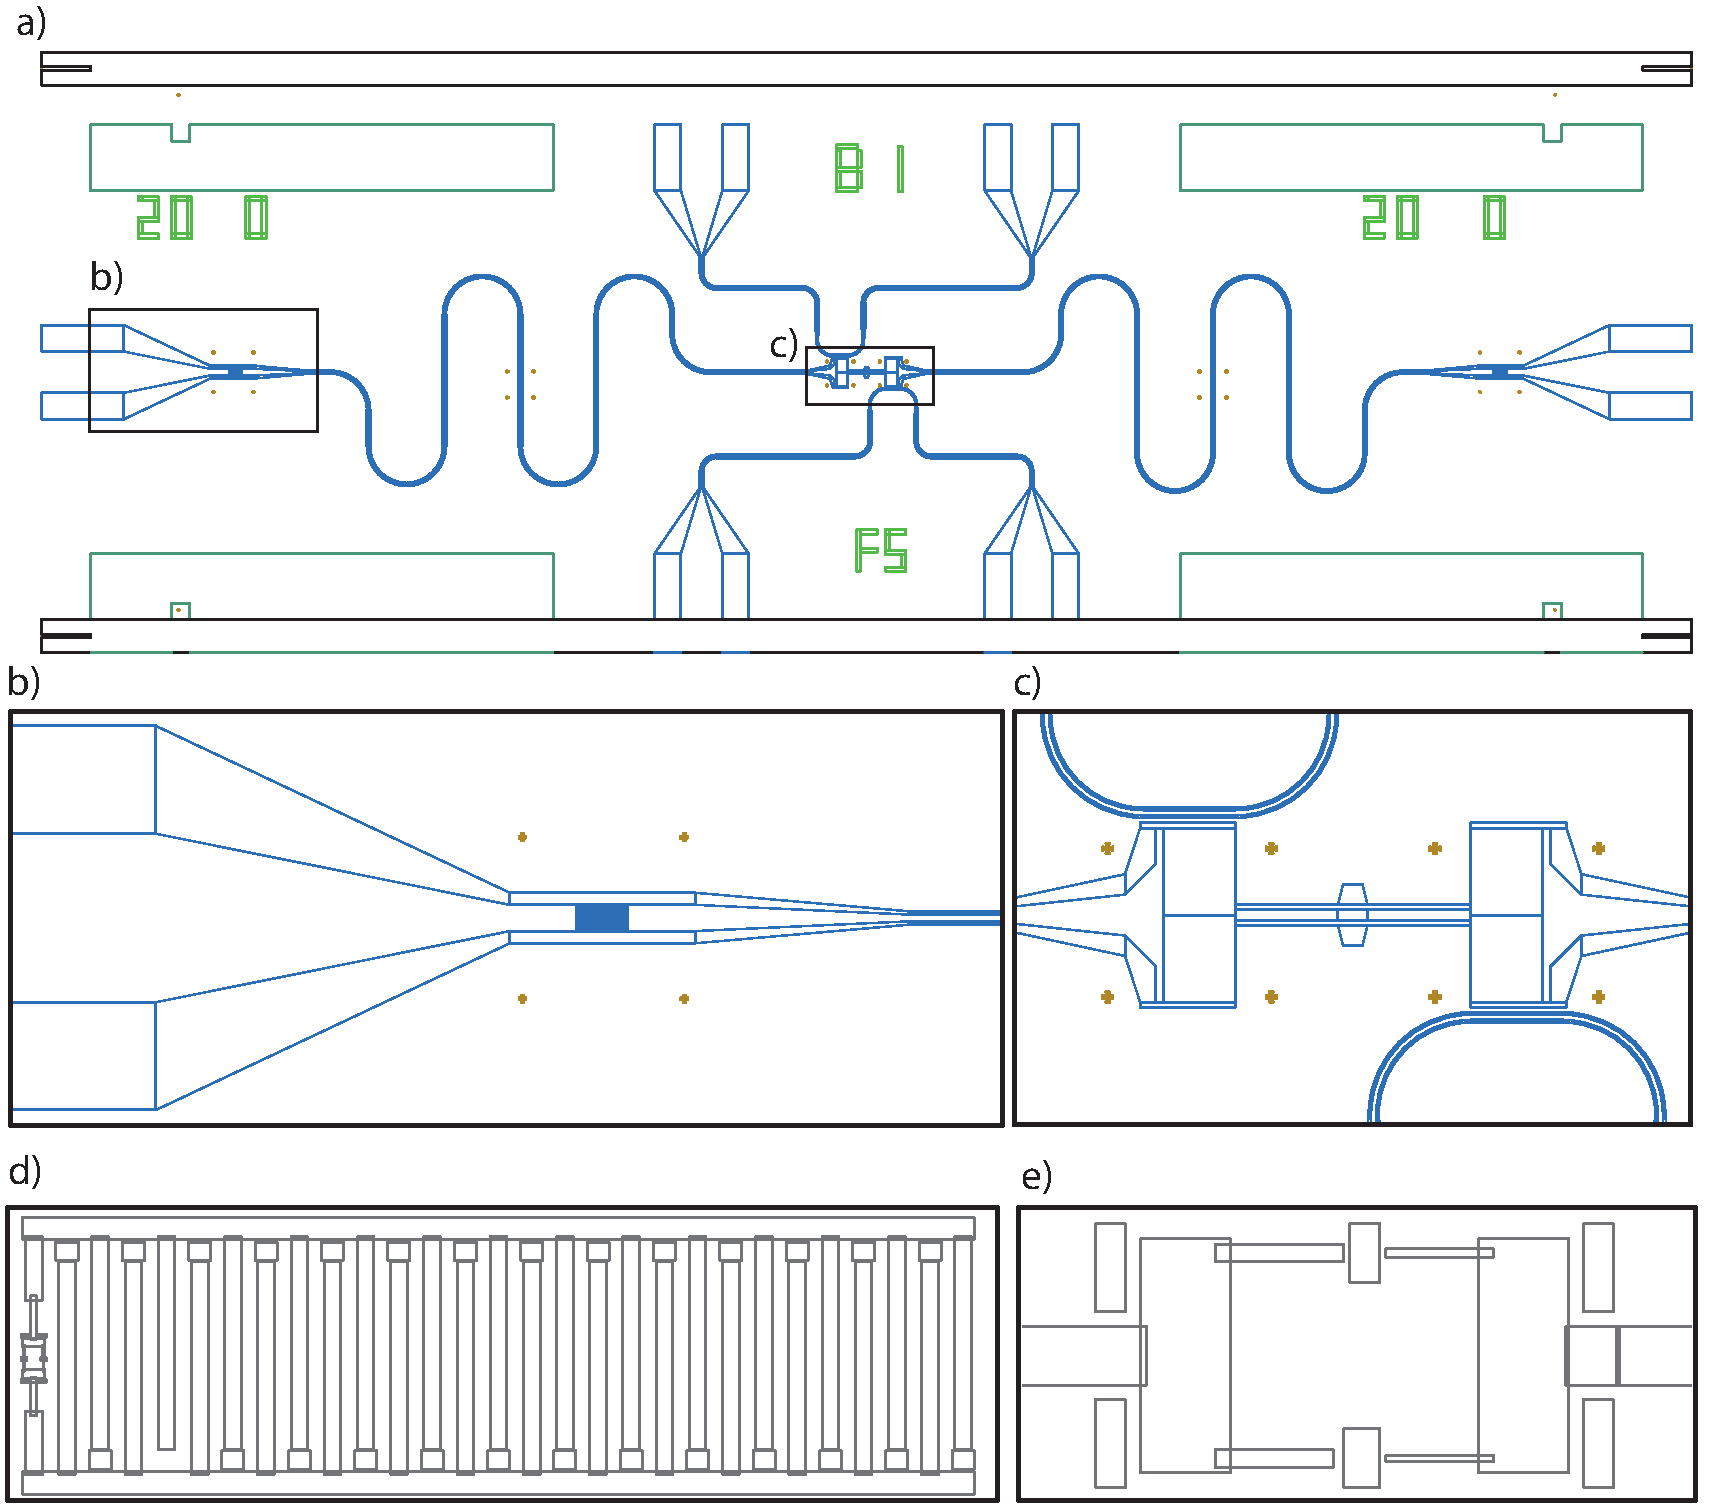
\includegraphics[width=\textwidth]{./material/figures/2-qubit-processor/fabrication/qubit_processor_layout}
	\caption[]{CAD layout of the implemented two-qubit processor, showing (a) the two CPW readout resonators and the two qubits with their adjacent fast flux lines, (b) the input capacitor of a resonator, (c) the two transmon housings in the center of the chip and the active section of the flux lines, (d) a transmon pattern for e-beam litghography, and (e) a more detailed view of the transmon's SQUID pattern.}
	\label{fig:processor_fabrication}
\end{figure}

After having chosen a set of sample parameters, it remains to find a physical implementation of the design that we can realize. In this section we discuss therefore the layout design of the qubit processor. From the beginning, we restrict our discussion to lithographically fabricated circuits on a chip, disregarding recent approaches to the realization of superconducting qubits and resonators using 3D microwave cavities \citep{paik_observation_2011}.

\smallskip

The readout resonator can be realized as a lumped-elements LC resonator or as a transmission line resonator. In the original approach to CQED \citep{wallraff_strong_2004}, a coplanar waveguide (CPW) resonator was used. Distributed microwave resonators such as CPW resonators are often advantageous since they can be fabricated with a high intrinsic quality factors \citep{megrant_planar_2012,creedon_high_2011,wang_improving_2009,barends_minimal_2010}, although recently large progress has been made concerning the quality factors of discrete LC resonators as well \citep{khalil_loss_2011}. Also, the isolation between the input port of the distributed resonator and the qubit electrode to which the open end of the resonator is coupled is high, whereas for a discrete LC resonator a significant capacitive coupling between the input port of the resonator and the qubit can exist, which is unwanted since it would cause additional relaxation. For this work, we therefore chose a distributed design using a $\lambda/2$ CPW resonator. The open port of the resonator is capacitively coupled to one of the qubit electrodes to achieve the desired coupling factor $g_{01}$. Figure \ref{fig:processor_fabrication} summarizes the layout of the qubit chip.

\smallskip

The flux lines can be realized in several ways. For our processor, we choose a simple 50 $\Omega$ CPW transmission line passing nearby the qubit SQUID at a distance of $d\approx 12\;\mathrm{\mu m}$. We eliminate the unwanted shielding currents in the ground planes by removing the ground plane between the qubit and the central conductor of the flux line, as shown in figs. \ref{fig:qubit_chip_photos}b and \ref{fig:sonnet_generated_model}a. By doing this, we also increase the capacitive coupling between the line and the qubit electrodes, thereby increasing the charge relaxation rate through the flux line. However, as discussed in section \ref{section:relaxation_through_charge}, this effect is negligible. The flux line can be terminated either directly at the 20 mK stage by wire-bonding it to the ground plane of the chip, or by connecting it to a matched impedance at the 4 K stage of the cryostat. Alternatively, we can also feed back the flux signal to room temperature, which is useful for e.g. measuring the response function of the line.

\smallskip

For the Transmon qubit itself, we need to fabricate a large shunt capacitance $C_J$ in order to achieve the desired charging energy. We implement this capacitance as an interdigitated planar capacitor that we pattern together with the qubit junctions using electron-beam lithography. The Josephson junctions of the qubit are realized in a SQUID geometry with a loop area of $A\approx 16\;\mathrm{\mu m}^2$ and are fabricated using double-angle shadow-evaporation of Aluminium.

\section{Electromagnetic Simulation of the Qubit-Chip}

\begin{figure}[ht!]
	\centering
	\includegraphics[width=\textwidth]{./material/figures/2-qubit-processor/sonnet_model}
	\caption[]{a) Schematic of the simulated chip geometry, showing the two coupled Transmon capacitances and the couplings to the readout resonators. b) Detailed view of the qubit coupling capacitance. c) SONNET generated equivalent model of the simulated geometry. d) Equivalent coupled Transmon circuit model. For the geometry shown, the obtained circuit parameters are $C_{g1}=C_{g2}=13.8\;\mathrm{fF}$, $C_{qq}=0.13\;\mathrm{fF}$, $C_{J1}=C_{J2}=52.2\;\mathrm{fF}$, $L_{J1}=L_{J2}=5.7\;\mathrm{nH}$.}
	\label{fig:sonnet_generated_model}
\end{figure}

We use a commercial software package for electromagnetic simulation (SONNET) to simulate individual parts of the chip an obtain the transmission coefficients between all relevant circuit components and an equivalent lumped-element model of the circuit. Using this equivalent model we calculate all relevant capacitances and inductances. We can then iteratively adapt the geometry of individual elements in order for them to match the designed parameter values. Figure \ref{fig:sonnet_generated_model}a/b shows an example of a circuit geometry used in the simulation, fig. \ref{fig:sonnet_generated_model}c shows the circuit model generated by this method and fig. \ref{fig:sonnet_generated_model}d the mapping of this model to a simplified circuit consisting of two capacitively coupled Transmon qubits.

\smallskip


We can also simulate the Transmon qubits as harmonic oscillators by modeling their Josephson junction as an inductance that matches the Josephson inductance of the junction, as given by eq. (\ref{eq:josephson_inductance}). By simulating the resonance curve of this harmonic resonator and calculating the corresponding quality factor $Q$, we can estimate the relaxation rate of the qubit through the gate circuit. We can also obtain an estimate of the coupling strength between the two qubits by simulating them as two coupled, linear resonators. We can obtain the impedance seen by the qubit through the gate circuit by this method as well, thereby being able to calculate the corresponding qubit relaxation rate.

\section{Fabrication}

\begin{figure}[p!]
	\includegraphics[width=1\textwidth]{"./material/figures/2-qubit-processor/processor photos"}
	\caption{Scanning electron micrographs of the fabricated two-qubit processor chip. a) Stitched together micrograph of the whole chip, showing the two readout resonators coupled to their transmission lines, the two capacitively coupled transmons, and the fast magnetic flux lines attached to each qubit. b-g) detailed views showing varous part of the chip: note that the aluminum electrodes are barely visible compared to the niobium ones that benefit from a much higher contrast. b) Flux line close to one of the qubits. The ground plane between the line and the qubit has been removed to suppress spurious shielding currents when sending fast flux pulses. c) Transmon qubit in its resonator housing. The left electrode is the center line of the resonator whereas the right one belongs to the coupling capacitor d) The two-qubit coupling capacitance. e) qubit SQUID loop with its two Josephson junctions. f) The CJBA Josephson junction. g) The readout resonator input capacitance.}
	\label{fig:qubit_chip_photos}
\end{figure}

We fabricate the processor on a high-resistivity silicon substrate with a 50 nm thermal oxide layer. First, we depose 150 nm of Niobium by magnetron sputtering. Afterwards, we spin a photo resist and define an etch mask through optical lithography. Then we dry-etch in a $\mathrm{SF}_6$ plasma, defining the readout resonators, transmission lines and qubit flux lines on the chip. This optical patterning is performed for the wafer as a whole. Afterwards, we spin a bilayer of MAA/PMMA electron beam resist (with typically $1050\;\mathrm{nm}$ of MMA and $115\;\mathrm{nm}$ of PMMA thickness). Then the wafer gets diced and the qubits and JBA junctions are patterned per chip using electron beam lithography, using a double-angle shadow evaporation technique to define the Josephson junctions and capacitances on the chip. The e-beam resist is then lifted off chemically in an Acetone bath. We characterize the chip optically afterwards. In addition, we place ``twin'' structures of the Transmon qubits and the JBAs on each chip that we can use to measure their normal state resistance at room temperature in order to obtain an estimate of the corresponding resistance of the real structures. Giving the normal-state resistance of a Josephson junction we can calculate the Josephson energy by using the Ambegaokar-Baratoff relation
%
\begin{equation}
E_J = \frac{\phi_0 \pi\Delta}{2e R_n},
\end{equation}
%
where $E_J = \phi_0 I_c$. When measuring $R_n$ at room temperature, a corrective factor of $\approx 17\%$ has to be applied to the resulting value of $E_J$ to account for variations in $R_n$ with temperature. 

\smallskip

Following we discuss the detailed procedure followed for fabrication of the two-qubit processor chip.

\begin{enumerate}
\item \textbf{Niobium Sputtering}: Deposit 150 nm Niobium at an argon pressure of 1.25 mbar and a power of 0.66 W/cm$^2$ with a 5 minute pre-deposition and $\approx$ 2 min 20 sec deposition time.
\item \textbf{Spinning of Photo-Resist}: Spin S1813 + Shipley Primer at 6000 RPM for 60 sec, bake at 115 ° C for 1 min 15 sec.
\item \textbf{Photo Lithography of Resonators}: Expose the wafer through a contact mask at 5 mW / cm$^2$ for 30 sec.
\item \textbf{Development}: Develop in pure MF 319 for 50 s.
\item \textbf{Reactive Ion Etching}: Pump the RIE chamber to $P\le 4\times 10^{-5}$ mbar. Etch using 20 cc of SF$_6$, 10 cc Ar and 2 cc O$_2$ at a pressure of $\approx$ 0.013 mbar at a power of 50 W and a voltage of 150 V. The total etch time should be $\approx $ 60 sec + 10 sec for the finish. Remove the resists in warm acetonee (40 °C) for at least 10 min, possibly clean further in an ultrasonic bath.
\item \textbf{Niobium Surface Regeneration}: Pump the RIE chamber  to $P\le 4\times 10^{-5}$ mbar, etch using 20 cc of SF$_6$, 10 cc Ar at $\approx$ 0.0133 mbar, 50 W and 150 V for 8 sec.
\item \textbf{Electron Resist Spinning}: Spin twice an MAA EL 10 layer at 2000 RPM for 60 sec, 6000 RPM for 2 sec. Bake after each step at 170 °C for 60 sec. Spin PMMA 950k A3 at 4000 RPM for 60 sec, 6000 RPM for 2 sec. Bake at 170 °C for 20 min. This should yield $\approx 1050$ nm of MAA and $110$ nm of PMMA (verify using interferometer).
\item \textbf{Dicing}: Dice the wafer using either a diamond cutter or wafer saw.
\item \textbf{Electron Beam Lithography of Transmons and CJBA junctions}: Clean the chip in iso-propanol (possibly in ultrasound) for less than 2 minutes. Perform electron beam lithography at a dose of $\approx$ 250-320 $\mathrm{\mu C}/cm^2$. Develop the chip in a 1:3 acetone/iso-propanol solution for 50 sec.
\item \textbf{Aluminum Deposition}: Put the sample in the evaporation chamber and pump to $P<10^{-6}$ mbar. Ion mill the sample at the two evaporation angles (typically $\pm 22\deg$) with 500 eV neutralized argon ions at the dose of $2\cdot 10^{15}$/cm$^2$. Deposit first aluminum layer at a rate of 1 nm/sec. Oxidize at an adequate oxygen pressure (typically 15 - 25 mbar) for 10 min. Deposit the second aluminum layer at 1 nm/sec.
\item \textbf{Lift-Off}: Put the chip in a heated Acetone bath at 65 °C for at least 5 min. Rinse in Iso-Propanol. Thermally stabilize the chip at 100 °C for 1 min.
\end{enumerate}


\chapter{Measurement Setup \& Techniques} \label{chapter:measurement}

In this chapter we discuss the measurement setup and techniques used in our experiments. Our setup consists of the qubit chip presented in chapter \ref{chapter:design}, hold at the 20~mK stage of a He$_3$/He$_4$ dilution refrigerator and connected to a signal generation and measurement chain including cryogenic microwave components and room temperature electronics. We describe below how the processor chip is mounted, as well as the individual parts of the signal  and measurement chain, putting emphasis on microwave pulse generation. Afterwards we briefly discuss the calibration and compensation techniques that we use to correct signal imperfections when generating qubit drive and flux signals. Finally we introduce the different measurement protocol used for driving and reading the qubit, as well as for determining all relevant qubit parameters such as frequency, anharmonicity, and relaxation and dephasing times.

\smallskip

\section{Chip mounting}

\begin{SCfigure}[1][ht!]
	\centering
		\includegraphics[width=0.6\textwidth]{"./material/photos/sample holder/sample_holder"}
	\caption[]{Chip mounting. Complete sample-holder (a), cover part as seen form below (b), and bottom part (c) with the mounted PCB carrying the qubit chip and the mini-SMP connectors. (d)  chip  wire-bonded to the PCB. Wire bonds to four CPW lines can be seen on the top and bottom of the picture, as well as on-chip bond wires reconnecting separated grounds inside the chip. The whole sample holder is screwed to the 20~mK stage of the dilution refrigerator.}
	\label{fig:pcb_and_sample_holder}
\end{SCfigure}

Chip monting is illustrated in  fig. \ref{fig:pcb_and_sample_holder}. The chip is first fixed to the lower part of the sample holder using a wax melting at 80°C. It is placed in a groove whose depth matches the height of the silicon chip, such that the top part of it is at the level of the surface of the sample holder after mounting. We use six small microwave PCBs, each equipped with a $50\;\Omega$ coplanar waveguide and a right-angle mini-SMP connector, which are also placed in matched grooves on the sample holder, as shown in fig. \ref{fig:pcb_and_sample_holder}c. The PCBs are made of TMM10, which has a dielectric constant of 10, close to that of the silicon chip, are metallized on both sides with gold-coated copper and have vias to connect the metal layers on both sides. The three electrodes of each CPW line on the chip are wire-bonded to their counterparts on the PCBs using aluminum wires of 50 µm diameter. In addition, on-chip bonded wires are used to reconnect separated parts of the ground plane that are initially isolated from each other because of the circuit topology, as shown in fig. \ref{fig:pcb_and_sample_holder}d. This is important in order to avoid spurious on-chip resonances in the relevant frequency window, i.e. below 10 GHz \citep{schuster_circuit_2007}.

The lower part of the sample holder with the chip and the small PCBs is then mounted to the gold-coated top part as shown in fig. \ref{fig:pcb_and_sample_holder}a/b, which thermally anchors the chip to the mixing chamber of the refrigerator, shields it from electromagnetic noise and encloses it in a conducting cavity that is small enough to suppress box resonances in the relevant frequency window. Grooves in the top part of the sample holder, shown in fig. \ref{fig:pcb_and_sample_holder}b, provide the necessary open space above the qubit chip and the six coplanar waveguides.

The whole sample-holder is mounted in the refrigerator by screwing it around a small coil that sits inside the cover and produces a DC magnetic field perpendicular to the chip. The distance between the chip and the lower end of the coil is less than 3 mm.

\section{Signal Generation \& Acquisition}

\begin{figure}[ht!]
	\centering
		\includegraphics[width=1.\textwidth]{"./material/figures/2-qubit-processor/measurement setup"}
	\caption[The measurement setup used for the two-qubit experiments]{Measurement setup used for the two-qubit experiments. The very same drive and readout setup is used for both qubits, so that only one exemplary is shown. The role of each line is indicated on top, and  the relevant parameters indicated beside each component, including the wire and cable materials. Elements shown are attenuators, low pass or bandpass filters, circulators and isolators, microwave amplifiers, IQ mixers, microwave and arbitrary waveform generators,and an acquisition board and a spectrum analyzer. }
	\label{fig:measurement_setup}
\end{figure}

Figure \ref{fig:measurement_setup} shows the wiring of our experiment from room temperature down to the 20~mK stage. Except for the small coil that is shared by both qubits, the rest of the circuitry is duplicated for each of them and only one exemplary is shown on the figure. One can see the bifilar dc flux line and a fast coaxial 50~$\Omega$ flux line on the left, as well as a set of 50~$\Omega$ coaxial microwave drive and readout lines on the right. Lossy cables or wires made from special alloys such as CuNi, CuBe, stainless steel (SS) and manganin are used at the highest temperatures to minimize heat transfer between the different stages. Between 20~mK and 4~K, superconducting NbTi cables are used for the measurement lines because they have both a low thermal conductivity and a low microwave attenuation. Semi-flexible Cu cables are used at 20~mK.

\subsection{Driving and Measurement of the Qubits}

Each of the qubits together with its corresponding readout resonator is fitted with an individual fast flux , drive, and measurement circuit. The microwave and arbitrary waveform generators used to control the experiment, as well as the acquisition systems, are all phase-locked using 10MHz external clocking.
At room temperature we generate qubit and readout resonator drive waveforms using phase-locked single-tone microwave sources whose continous output is mixed with fast control pulses generated by two arbitrary waveform generators (more details in the next section). The qubit drive and readout drive signals are then combined on a single line per qubit and sent to the chip through a series of cryogenic attenuators and filters. A cryogenic circulator at 20~mK routes the incoming pulses to the qubit chip, where they are sent to the qubit readout resonator and finally reflected by it. The reflected signal passes again through the circulator and gets routed through a double isolator and a band-pass filter to a cryogenic high electron mobility amplifier (HEMT) with a gain of 40~dB. The amplified signal gets then transmited to the room temperature electronics, where it is filtered and amplified further by more than 50~dB. Finally, the signal is demodulated using a two-quadrature mixer and a continous microwave reference tone (local oscillator), the two resulting quadrature being further amplified, filtered below 200MHz and  fed to two channels of  a 4-channel ADC board.
High-frequency and DC flux pulses are generated using an arbitrary waveform generator at room temperature. The signal is then sent to the qubit chip through a 20~dB attenuator, through a conventional Microtronics low-pass filter of the reflective type, and through a custom-made high-frequency powder filter that uses an absorptive material (Eccosorb) to attenuate high-frequency noise. After passing through the transmission line on the qubit chip, the outgoing flux signal gets routed to room temperature through a transmission line identical to the input line. There, the signal can be measured, which is useful for characterizing possible signal imperfections caused by the non-ideal character of the line.

\subsection{X-Y Pulse Generation by Microwave Single Sideband Mixing}

As briefly mentionned above, a single-sideband mixing technique is used to generate the qubit X and Y driving pulses. More precisely, each qubit has its own IQ mixer driven with a continous single-frequency microwave tone and two synchronized intermediate frequency control signals generated by an arbitrary waveform generator (Tektronix AWG5014b). In general, when feeding a signal $LO(t) = i_0 \cos{(\omega_{LO} t )}$ to the LO port of an IQ mixer and two signals $I(t)$, $Q(t)$ to its I and Q ports, we obtain a signal

\begin{equation}
RF(t) = I(t)\cos{(\omega_{LO} t)}+Q(t)\sin{(\omega_{LO} t)} \label{eq:iqMixer}
\end{equation}
at the RF output port. (Since the IQ mixer that we use is a passive reciprocal device, one can as well feed two input signals to the LO and RF ports and obtain the demodulated signal quadratures at the I and Q ports after filtering, a technique that we make use of in our qubit readout scheme). Typically we use heterodyne single sideband mixing to generate driving pulses that are tunable in frequency with respect to the local oscillator (carrier  frequency), over the mixer bandwidth (several hundreds of MHz): Ideally, the I and Q signals should have the form $I(t)=s(t)cos(\omega_{IF} t-\phi)$ and $Q(t)=s(t)sin(\omega_{IF} t-\phi)$ in order to obtain an output pulse $RF(t)=s(t)cos[(\omega_{LO}-\omega_{IF})t +\phi]$ that will induce a rotation of the qubit around axis $X_{\phi}$ laying in the equatorial plane of the Bloch sphere and making an angle $\phi$ with the $X$ axis. The phase reference of the driving pulses is thus defined by both the carrier phase and the common starting time of the I and Q waveforms with respect to the carrier. Both quantities have to be kept constant over subsequent sequences. In addition, when performing experiments on multiple qubits, the phase differences between the reference phases of each qubit must also be conserved.  We explain below in the section devoted to synchronization how these phase references are maintained. In the expression above $s(t)$ is the envelope of the pulse, the area of which defines the angle of rotation. For small rotation angle, we choose for $s$ a Gaussian shape of the form
%
\begin{equation}
s(t) = s_0\cdot\exp{\left[-\frac{(t-t_0)^2}{2\sigma_t}\right]}
\end{equation}
%
with "rise time" $\sigma_t=3\;\mathrm{ns}$. The advantage of using such a Gaussian pulse \citep{bauer_gaussian_1984} is that its Fourier transform is again a Gaussian, which, in contrast to a rectangular pulse, does not exhibit side lobes in the frequency domain and thus minimizes the leakage to higher Transmon levels discussed in section \ref{section:charge_driving}. To increase the Rabi angle of such a pulse, we just change its amplitude as far as it does not saturate the IQ mixer. For larger Rabi angles we simply add a flat plateau between the Gaussian rise and fall.

\begin{figure}[ht!]
	\centering
		\includegraphics[width=0.7\textwidth]{"./material/figures/measurement/mixer_imperfections"}
	\caption[...]{Illustration of the method used to measure and correct the imperfect behavior of the IQ mixers used for  our heterodyne single-sideband generation of the qubit drives: the leakage of the LO signal to the RF port is measured continuously with a spectrum analyzer and is minimized by tuning the two offset voltages $I_0$ and $Q_0$ at the I and Q ports. To correct phase and amplitude errors during heterodyne mixing, we then add two sideband signals to the IF ports and minimize iteratively the measured RF power at $\omega_{LO}+\omega_{IF}$ by tuning tha amplitude and phase of two correction waveforms added to the I and Q ports.}
	\label{fig:iq_mixer_correction}
\end{figure}

We now discuss imperfections of commercially available IQ mixers, which always deviate from the ideal behavior given by eq. (\ref{eq:iqMixer}). Typical imperfections include large insertion losses --i.e. loss of  power between the different ports of the mixer--, RF signal leakage at zero IQ-input, and frequency-dependent phase and amplitude errors of the mixed sideband signals. In order to achieve reliable single-qubit operations we need to correct these errors, as illustrated in Fig. \ref{fig:iq_mixer_correction}. The signal leakage consists in a small part of the LO signal leaking through to the RF port even when the IQ inputs are zeroed. This leakage can be compensated by adding LO frequency $\omega_{LO}$ dependent DC offset voltages to the IQ ports. The appropriate offsets can be determined by applying a continuous signal at a frequency $\omega_{LO}$ to the LO port and minimizing the measured signal power at the RF port. Using this method, the leakage power can be reduced down to -80 dBm.

To correct the sideband amplitude and phase errors we apply another correction procedure that we outline here. We first introduce the notation
\begin{equation}
A(t) = I(t)+iQ(t) = a(t)\exp{[-i \phi(t)]} \label{eq:iq_if_input}
\end{equation}
for any composite I and Q signal. We then consider such a signal at a single sideband frequency $\omega_{IF}$ and at a fixed complex amplitude $a(t)=a= a_0\exp{(i\phi_0)}$ such that $A(t) =a \exp{[-i \omega_{IF} t]} $. The effect of the gain and phase imperfections are responsible for a spurious additional output signal at the mirrored sideband frequency $-\omega_{IF}$ with respect to the carrier. This unwanted signal would be obtained in a perfect mixer with an IQ signal $\epsilon(\omega_{IF},\omega_{LO})A^*(t)$. We can thus remove it by adding a small correction $c(\omega_{IF},\omega_{LO})A^*(t)$ to our IQ input signal. The complex-valued correction coefficient $c(\omega_{IF},\omega_{LO})=|c|\exp{(i\angle c)}$ usually depends both on the LO frequency $\omega_{LO}$ and the sideband frequency $\omega_{IF}$. We thus determine it  by generating a continuous single sideband at frequency  $\omega_{LO}-\omega_{IF}$  and by finding  iteratively the  $c(\omega_{IF},\omega_{LO})$ that minimizes the amplitude of the unwanted sideband at $\omega_{LO}+\omega_{IF}$, measured with a spectrum analyzer (see Figs.  \ref{fig:measurement_setup} and \ref{fig:iq_mixer_correction}). Both the offset and the sideband-amplitude and -phase corrections have been automated using our data acquisition software. By using this optimization techniques we can lower the amplitudes of the $\omega_{LO}$  and $\omega_{LO}+\omega_{IF}$ peaks down to 80 dB and 70 dB below the targeted sideband at $\omega_{LO}-\omega_{IF}$, respectively.

\smallskip

Finally, it is important to tolerate the maximum and minimum absolute ratings for the signals applied to the I/Q  as well as LO and RF ports of the mixer in order to avoid saturation and nonlinear response. For the mixer that we use in our setup (Hitite HMC 525), the maximum input powers are given as 20 dBm for the RF and I/Q ports and 27 dBm for the LO port. In addition, the maximum tolerable DC current of the mixer at the I/Q ports is limited to 3 mA, which restricts the DC offset voltage that we can supply to the mixer.

\subsection{Fast Magnetic Flux Pulse Generation and Calibration}

The fully symmetric coaxial line used for sending fast magnetic flux pulses to one of the qubits has been described above and is shown on Fig. \ref{fig:measurement_setup}. Appendix \ref{} contains additional details on the fabrication and frequency attenuation of Eccosorb filters. The low-pass filtering of the line is optimized to reduce high-frequency noise as much as possible while letting the line pass pulses with 2-3 ns risetime. Consequently, the pulse  distorsion by the line is not negligible. Another important imperfection in our pulse generation is the finite bandwidth of the arbitrary waveform generator we use ( Tektronix AWG5014B). It is about 500MHz and some ringing is observed at a few percent level for square pulses with risetimes below 10 ns. For compensating all these imperfections, we measure the frequency response of each part of the whole circuit with our 1 GHz bandwidth acquisition system. A step function with 2 ns risetime and 1ns/sample is programmed on the AWG and measured at the output of the flux line. This allows us to obtain the response function of the generator (DAC) and of the input line. We then model the whole chain as shown on Fig. \ref{fig:FluxLineResponseFunction}a and use the same response function for the identical input and output lines. The Fourier transform of the measured signal at the end of the output line is given as

\begin{SCfigure}[1.0][ht!]
	\begin{tabular}{l}
	 a) \\ \includegraphics[width=0.5\textwidth]{"./material/figures/measurement/fluxline_model"} \\
	 b) \\ \includegraphics[width=0.6\textwidth]{"./material_thesis/fluxline response/response"} \\
	 c) \\ \includegraphics[width=0.6\textwidth]{"./data/ct5/2010_06_15 - fluxline response/test_measurement_modified"}
	 \end{tabular}
	 \caption[]{a) Schematic of the flux line chain used in our setup. The flux signal is generated by a DAC, fed through the input line to the sample, returned to room temperature through the output line and ditigized by an ADC. b) Measured response functions of different parts of the flux line, showing the response of the DAC and ADC circuits and of the input part and the full flux line. c) Illustration of the signal correction method. We generate a desired waveform (in red) without applying any correction, measure the arriving signal at the sample (in magenta), calculate the response function of the line and generate a corrected signal (in green), which we measure again at the sample (in blue). The corrected signal corresponds to a good degree to the desired input signal.}
	 \label{fig:FluxLineResponseFunction}
\end{SCfigure}

%
\begin{equation}
\chi_{\mathrm{fl}}(\omega) = \chi_{signal}\cdot \chi_{DAC}\cdot \chi_{\mathrm{input}}\cdot\chi_{\mathrm{output}}\cdot\chi_{ADC}, \label{eq:flux_response}
\end{equation}
%
with $\chi_{\mathrm{signal}}$ the Fourier transform of the ideal input signal, $\chi_{ADC}$ and $\chi_{DAC}$ the response functions of the DAC and ADC (which we measure independently), and $\chi_{\mathrm{input}}=\chi_{\mathrm{output}}$ the response function of the input and output transmission lines. By measuring $\chi_{\mathrm{fl}}$, substracting the ADC and DAC responses from it and assuming that $\chi_{\mathrm{input}} \approx \chi_{\mathrm{output}}$, we obtain the input line response function $\chi_{\mathrm{input}}$. To correct the signal distortion seen by the qubit, we can then simply re-program the AWG with a corrected wavefunction with Fourier transform 
%
\begin{equation}
\chi_{\mathrm{signal}}^{\mathrm{corr}} = \chi_{\mathrm{signal}}\cdot (\chi_{DAC}\cdot\chi_{\mathrm{input}})^{-1}\cdot \mathrm{G}(\omega,\omega_{co}).
\end{equation}
%
Here, $G(\omega,\omega_{co})$ is a Gaussian filter function with a cutoff frequency $\omega_{co}$ that we apply to the inverse measured response function to eliminate the distortion at high frequencies caused by the fact that we are not able to accurately measure the response function of the flux line above a certain frequency limit, due to the limited bandwidth of our digitizing board. Usually, we set this cutoff frequency to $\omega_{co}/2\pi=400\;\mathrm{MHz}$, which allows us to correct most signal distortion in the frequency window relevant to this work, i.e. up to half a GHz. Figure \ref{fig:FluxLineResponseFunction}b shows the measured response functions of the flux line and fig. \ref{fig:FluxLineResponseFunction}c shows an exemplatory measurement, where we first program an ideal waveform (in red) in the AWG, send it through the flux line, calculate the shape of the waveform at the sample (in magenta) by measuring the waveform at the output of the line and substracting the measured response functions of the ADC and the output line, then program a corrected waveform (in green) and finally measure the shape of this waveform at the sample again (in blue), which now corresponds closely to the ideal waveform.
 


\smallskip

After having corrected the response of the flux line by this technique, we can further reduce signal distortion by directly probing the flux seen by the qubit at a given time. For this, we apply a small test flux signal $\phi_{ext}^{fl}(t)$ to the qubit, measure its frequency $\omega_{01}(t)$ and reconstruct the flux from the previously measured  $\omega_{01}(\phi_{ext})$ curve. If the qubit frequency is chosen well away from its maximum and minimum frequencies (where $\gamma=\partial \omega_{01}/\partial \phi_{ext}^{fl} \ne 0$) and if the flux signal is comparably small, we can write the time-dependent qubit frequency as $\omega_{01}(t)=\omega_{01}^0+\gamma.\delta\phi_{ext}^{fl}(t)$. The frequency displacement of the qubit is thus proportional to the applied flux signal. Now, if we drive the qubit with a calibrated $X_\pi$ Rabi pulse at a given drive frequency $\omega_{d}$ at time $t_0$, the probability of finding it in state $\ket{1}$ afterwards is maximum if $\omega_{d}=\omega_{01}(t_0)$. Thus, by maximizing this probability as a function of $\omega_{d}$, we can reconstruct the flux $\phi_{ext}^{fl}(t_0)$ seen by the qubit at any given moment. Of course, the time resolution achieved with this method is limited to the pulse duration of the $X_\pi$ pulse, which is typicall $3-5\;\mathrm{ns}$. After having reconstructed the flux signal $\phi_{ext}^{fl}(t)$ seen by the qubit, we can again calculate its Fourier transform and correct imperfections by changing the input signal that we send.

\subsection{Microwave and DC Pulse Synchronization}

In our experiment, each qubit possesses two microwave sources that generate the continuous tones for drive and readout. The two fast pulse signals mixed with the two driving tones of the two qubits are generated by a single 4-channel arbitrary waveform generator (AWG5014B). A second AWG generates the flux pulses for the two qubits. The measurement of the reflected and demodulated readout signal of both qubits is done by a single ADC card. All these different signal generators and measurement devices need to be synchronized in order to keep the relative phases and time differences between them constant over successive individual runs of our experiment. For this, we use a 10 MHz frequency reference chain, whose master clock is generated by the AWG that is responsible for generating the qubit drive pulses. The reference signal is then passed on to all microwave sources and signal generators as well as oscilloscopes, spectrum analyzers and ADC cards in our setup. In addition, to avoid random phase-jitter between the signals of the two microwave sources that generate the drive pulses of the two qubits, their drive frequencies need to be chosen such that they correspond to a multiple of the repetition frequency of the master AWG, which is typically 50 kHz. If this condition is met, the relative phases between the two microwave signals is conserved between individual runs of an experiment, which is crucial when performing measurements that are sensitive to this phase such as quantum state tomography two entangled qubits. In addition, a 1 GHz phase synchronization chain is used to phase-lock the two microwave generators and reduce the phase drift between them.

\section{Measurement Techniques}

In this section, we discuss the techniques used to manipulate and characterize our two-qubit processor. We address qubit readout and describe how the relevant qubit parameters are determined.

\section{Qubit Readout} \label{section:qubit_readout}

\begin{figure}[ht!]
\centering
\includegraphics[width=\textwidth]{./material/figures/measurement/readout}
\caption[]{a) Microwave pulse envelope used for exciting the CJBA at readout.The pulse consists of a measurement part with amplitude $h_m$ and a latching part with ampliude $h_l=0.8-0.9h_m$. To determine the state of the resonator during the latching interval, the quadratures I and Q of the reflected signal are averaged over the time window $t_m$. b) Bimodal distribution of the time-averaged $(I,Q)$ values obtained for a readout power close to the bifurcation threshold . The red dotted line perpendicular to the principal axis joining the two modes of the distribution and going through the mean quadratures $(I_0,Q_0)$ provides an optimal separation between the two clusters corresponding to the L and H states. c) Histograms of the signal projected on the principal axis (red line), revealing a switching probability of 84\% for the  example shown.}
\label{fig:readout_bringup}
\end{figure}



The general principle of the CJBA readout used in this work is described in section \ref{section:cjba}. Here we explain how we choose its frequency $f_d$ and drive amplitude $a_d$. To bring up the readout, we first determine by reflectometry the resonance frequency $f_r$ of the CJBA in its linear regime, with the qubit in state $\ket{0}$ and largely detuned from the resonator. We then choose a relative drive detuning $\Omega=2Q(f_d/f_r-1)>\sqrt{3}$  (between 2 and 10 in practise, i.e. between 12 and 60 MHz ) at which the bistable regime is accessible (see Fig. \ref{}). The continous drive tone at $f_d$ is then split on two lines, one of them being mixed with the dc envelope coming from the AWG and sketched on fig. \ref{fig:readout_bringup}a. We then attenuate the resulting drive signal using a tunable attenuator at room temperature and send it to the CJBA. The reflected and amplified signal is then demodulated with the continous drive present on the second line after the splitter, using an IQ demodulator. The resulting I/Q quadratures are further amplified, low-pass filtered at 200 MHz, and get digitized by the ADC card at a sampling rate of 1 GSample/s during the time window $t_m=1-2\mu$s sketched in fig. \ref{fig:readout_bringup}a. The digitized I/Q signals are then averaged over the whole measurement window to obtain a single measurement point in the IQ plane.  This sequence is repeated a large number of times (typically $10^4$) to obtain a statistical distribution of IQ points. We then repeat this procedure for various values of the input attenuation, each time calculating the estimated variance $\hat{\sigma}_{IQ}^2=\sum\limits_i ((I_i-\bar{I}_i)^2+\sum\limits_i (Q_i-\bar{Q}_i)^2)/n$ of the distribution. When starting with a high attenuation and reducing it, the input power sent to the CJBA will at some point be sufficient to make it switch from the L to the H state, thereby changing the phase and consequently the I and Q average values of the distribution. Since the switching is a stochasic process, we will observe two families of points close to the transition power. At an input power where approximately 50 \% of switching occurs, the variance $\sigma_{IQ}^2$ of the obtained IQ data points will be largest, as shown in fig. \ref{fig:readout_bringup}b. At this point, we substract the averages $(I_0=\sum\limits_i I_i / n,Q_0 = \sum\limits_i Q_i/n)$ from the data and perform a principal axis transformation, which diagonalizes their covariance matrix
%
\begin{equation}
\mathrm{var}_{IQ} = \left(\begin{array}{cc}\mathrm{var}(I) & \mathrm{cov}(I,Q) \\ \mathrm{cov}(I,Q) & \mathrm{var}(Q) \end{array}\right).
\end{equation}
%
Using this transformation, we project the measured (I,Q) points on the axis $\perp P$ joining the two sub-distribution, as shown in fig. \ref{fig:readout_bringup}, and obtain a bivaluated one-dimensional probability distribution. Then, the obtained offsets $I_0$, $Q_0$ and principal axis rotation angle $\alpha_{IQ}$ gives us the discrimination criterion $Q_L<Q_0+\tan{\alpha_{IQ}}(I-I_0)$ used to classify new data points as belonging to the L or H state at the chosen working point. Normally, if the measurement window $t_m$ is large enough and no retrapping occurs during the meausurement, the distributions corresponding to the L and H states will not overlap, yielding perfect discrimination between them, as shown on the figure.

\begin{SCfigure}[1][ht!]
\centering
\includegraphics[width=0.4\textwidth]{./material/papers/grover/figures/s_curves_example}
\caption{Exemplary S-curve measured for one of the qubit-readout. Shown is the switching probability $p$ of the CJBA as a function of the readout signal power, plotted for the different qubit states $\ket{0}$,$\ket{1}$ and $\ket{2}$. The readout contrast between different states is given as difference between the associated switching probability curves. Light and dark red arrows indicate the optimal working points where the $c_{01}$ and $c_{02}$ readout contrasts are maximum, respectively.}
\label{fig:s_curves_example}
\end{SCfigure}

\smallskip

After having determined the $I_0$, $Q_0$ and $\alpha_{IQ}$, we slightly tune the attenuation to obtain $\approx 20\%$  of switching. At this working point, the readout contrast of the CJBA is usually already sufficient to perform a simple qubit spectroscopy, as described in section \ref{section:qubit_spectroscopy} and calibrate a $X_\pi$ Rabi pulse, as described in section \ref{section:qubit_rabi}. After having done this, we calibrate and optimize each qubit readout by measuring the switching probability as a function of the input power while either leaving the qubit in state $\ket{0}$ or exciting it to the state $\ket{1}$. Fig. \ref{fig:s_curves_example} shows an example of such a measurement. Here, the difference $c_{01}$ between the two curves corresponding to the $\ket{1}$ and $\ket{0}$ states defines the input-power dependent readout contrast. The optimal  input power chosen for reading the qubit out is where the contrast is maximum. If desired, we also apply a $X_\pi^{10}\cdot X_\pi^{12}$ pulse sequence to the qubit to bring it into state $\ket{2}$ before readout. In this state, the dispersive shift of the resonator frequency is larger than in the state $\ket{1}$, therefore resulting in a larger readout contrast $\mathrm{max}(c_{02})>\mathrm{max}(c_{01})$, as shown in fig. \ref{fig:s_curves_example}. This shelving of state $\ket{1}$ to state $\ket{2}$ is advantageous when performing e.g. single-run quantum algorithms on the processor, as described in chapter \ref{chapter:grover_algorithm}.

\subsection{Qubit Spectroscopy} \label{section:qubit_spectroscopy}

\begin{figure}[h!]
\begin{center}
\begin{tabular}{l}
a) \\ \includegraphics[width=0.6\textwidth]{"./material/figures/measurement/qubit_spectroscopy"} \\
b) \\ \includegraphics[width=0.6\textwidth]{"./data/ct5/2011_04_21 - grover and tomo/example - qubit 2 spectroscopy"} \\
\end{tabular}
\end{center}
\caption[]{a) Qubit drive and readout pulse sequence used for qubit spectroscopy. b) Example of qubit spectrum showing the switching probability of the qubit readout when driving the qubit with 1 $\mu$s-long pulse as a function of the drive frequency. Low power spectroscopy (red points) shows only the $\ket{0}\to\ket{1}$ transition of the qubit at frequency $f_{01}$, wheras the 2-photon $\ket{0}\to\ket{2}$ transition at frequency $f_{02}/2$ is also observed at higher power (blue points). Lorentzian functions (lines) are fitted to these two spectroscopic lines.}
\label{fig:qubit_spectroscopy_example}
\end{figure}

In order to characterize the transition frequency and anharmonicity of the qubit we perform spectroscopic measurements. For this we drive the qubit with a long Rabi pulse (usually $> 1\;\mathrm{\mu}$s) at a frequency $\omega_d$. When the drive frequency $\omega_{d}$ is close to the $\omega_{01}$ frequency of the qubit, the drive pulse will induce a Rabi oscillation of the quantum state of the qubit. The induced rotation amplitude will be largest at $\omega_d=\omega_{01}$. Due to decoherence during the driven evolution, the maximum probability for measuring the qubit in the state $\ket{1}$ at the end of the pulse will be limited to 50 \%. By repeating the pulse sequence shown in fig. \ref{fig:qubit_spectroscopy_example}a for a range of drive frequencies $\omega_d$, a full spectroscopy of the qubit can be obtained. Fig. \ref{fig:qubit_spectroscopy_example}b shows an example of this, for different drive amplitudes. Here, the blue curve has been measured at $10\;\mathrm{dB}$ higher power than the red curve, which is sufficient to observe the two-photon $\ket{0}\to\ket{2}$ transition of the qubit at $f_{02}/2$. By fitting the two resonance curves with a Lorentzian model we obtain the qubit frequencies $f_{01}$ and $f_{02}/2$, and from Eqs. \ref{} the charging and Josephson energies of the qubit at the given working point.

\subsection{Rabi Oscillations} \label{section:qubit_rabi}

\begin{figure}[h!]
\begin{center}
\begin{tabular}{l}
a) \\ \includegraphics[width=0.6\textwidth]{"./material/figures/measurement/qubit_rabi_oscillation"} \\
b) \\ \includegraphics[width=0.6\textwidth]{"./data/ct5/2011_04_21 - grover and tomo/example - qubit 2 rabi"} \\
\end{tabular}
\end{center}
\caption[]{a) Qubit drive and readout pulse sequence used for measuring Rabi oscillations. b) Example of a measured Rabi oscillation showing the switching probability of the qubit readout when driving the qubit at $f_{01}$ with a Gaussian drive pulse of increasing effective duration t (points). The measurement results are not corrected for readout errors. The line is a fit by an exponentially decaying sine function.}
\label{fig:qubit_rabi_example}
\end{figure}

After having obtained the proper qubit transition frequency $f_{01}$, we calibrate Rabi pulses. For this, we  perform a Rabi oscillation experiment that consists in driving the qubit at $f_{01} $with pulses of increasing areas and in measuring its state immediately afterwards. Figure \ref{fig:qubit_rabi_example} shows the pulse sequence that we use and the resulting measurement data, the readout switching probability being expressed as a function of an equivalent pulse length at a nominal pulse height. to the experimental data. As can be seen, the amplitude of the Rabi oscillations gets damped as  $p(t)=p_0+{\Delta}p\cos{(\Omega t)}\exp{(-\Gamma_R t)}$ due to relaxation and dephasing during the driven evolution. Also, the maximum readout contrast is limited due to readout errors characterized in details in the next chapter. From the fit of the Rabi data we obtain the Rabi frequency $\Omega$, which we use to program precise single-qubit rotations in all our experimental sequences. Nota that due to the finite anharmonicity of the qubit, there is always a finite leakage to the second excited state $\ket{2}$, which we discuss later.

\section{Relaxation Time Measurement}

\begin{figure}[ht!]
\begin{center}
\begin{tabular}{l}
a) \\ \includegraphics[width=0.6\textwidth]{"./material/figures/measurement/qubit_t1_measurement"} \\
b) \\ \includegraphics[width=0.6\textwidth]{"./data/ct5/2011_04_21 - grover and tomo/example - qubit 2 t1"} \\
\end{tabular}
\end{center}
\caption[]{a) Qubit drive and readout pulse sequence used for relaxation time measurement. b) Example of relaxation time measurement showing the probability of measuring the qubit in state $\ket{1}$ as a function of the delay time between the preparation of the state $\ket{1}$ and the actual measurement of the qubit state (points). The line is a fit by a decaying exponential.}
\label{fig:qubit_t1_example}
\end{figure}

Having obtained the transition frequency $f_{01}$ and calibrated the Rabi frequency $\Omega$, we measure the relaxation time of the qubit. For this, we put the qubit in state $\ket{1}$ by applying a $X_{\pi}$ pulse and let it evolve freely afterwards for a given delay time before reading out its state, as shown in fig. \ref{fig:qubit_t1_example}a. As can be seen on fig. \ref{fig:qubit_t1_example}b, the probability decreases exponentially as a function of time. A fit of the function $p(\ket{1}) = p_0+p_a\exp{(-\Gamma_1 t)}$ to the data yields the qubit relaxation rate $\Gamma_1$ at the given working point. In the following chapter we measure in more detail the relaxation time of both qubits as a function of their transition frequency and their detuning from the readout resonator.

\section{Dephasing Time Measurement}

\begin{figure}[ht!]
\begin{center}
\begin{tabular}{l}
a) \\ \includegraphics[width=0.55\textwidth]{"./material/figures/measurement/qubit_ramsey_oscillation"} \\
b) \\ \includegraphics[width=0.6\textwidth]{"./data/ct5/2011_04_21 - grover and tomo/example - qubit 2 ramsey"} \\
\end{tabular}
\end{center}
\caption[]{a) Qubit drive and readout pulse sequence used in a Ramsey experiment. (b) Example of a measured qubit Ramsey experiment showing the switching probability of the qubit readout (points) at the end of the sequence. Fitting the resulting curve with an attenuated sine-wave model (line) yields the dephasing rate $\Gamma_{\phi}$ and the qubit frequency $f_{01}$ (see text).}
\label{fig:qubit_ramsey_example}
\end{figure}

We also characterize the dephasing of each qubit by performing a so-called {\it Ramsey fringe experiment}, consisting in two $Y_{-\pi/2}$ pulses separated by a delay time ${\Delta}t$ and a readout immediately afterwards, as illustrated  on Fig. \ref{fig:qubit_ramsey_example}a. We either choose microwave pulses detuned from $f_{01}$ by an amount ${\Delta}f$, or use resonant microwave pulses together with a flux pulse that shifts the qubit frequency by ${\Delta}f$ during the whole delay. After the first pulse the qubit is in state $1/\sqrt{2}(\ket{0}+\ket{1})$ and acquires  a phase  $\Delta \phi = 2\pi\Delta f \Delta t$ during the delay. The final state of the qubit after applying the second $Y_{\pi/2}$ pulse therefore becomes
%
\begin{equation}
\ket{\phi_f} =1/\sqrt{2} \left(\begin{array}{cc} 1 & 1 \\ 1 & -1 \end{array} \right)\cdot\left(\begin{array}{c} 1 \\ e^{i\Delta\phi} \end{array}\right) = \left( \begin{array}{c}  -\cos{\Delta\phi/2} \\ i\sin{\Delta\phi/2} \end{array}\right),
\end{equation}
%
and the probability $p=\cos^2{\Delta\phi/2}$ to measure state $\ket{1}$ oscillates with frequency $\Delta f$ as a function of the delay ${\Delta}t$ . Due to dephasing and relaxation during the free evolution, the amplitude of these oscillations will decay. As explained in section $\ref{}$, this decay takes the form $\exp{(-\Gamma_2 t)}$ with $\Gamma_2=\Gamma_1/2 +\Gamma_{\phi}$ if the noise responsible for dephasing is white at low frequency, or the form $\exp{(-\Gamma_1 t/2 )}\exp{(-B t^2)}$ if the noise has a 1/f dependance. Even if the main dephasing source is 1/f flux noise of microscopic origin, the decay of the Ramsey oscillations is close to an exponential due to the relaxation contribution. So in practise, we fit the Ramsey data by $a cos({\Delta}f.t)\exp{(-\Gamma_2 t)}$ and deduce an effective dephasing rate $\Gamma_{\phi}$.
Furthermore, the fit provides an accurate measurement of ${\Delta}f$ and consequently of the qubit frequency $f_{01}$, which is now known with a precision of $100\;\mathrm{kHz}$. 


\chapter{Characterizing the Two-Qubit Processor} \label{chapter:processor_characterization}

After having detailed the design of the processor and the measurement techniques employed in this work, we will now show how we can ``test drive'' it to show the basic functionality that we need to run meaningful quantum algorithms. In particular we show how we can implement a robust two-qubit quantum gate that we will use in the following chapter to run a real-world quantum algorithm on our processor.

\smallskip

We begin the chapter by discussing the measurement of the basic qubit and readout parameters. We will then give a detailed overview of the relevant decoherence times and readout fidelities of our processor at different working points and discuss our strategy for optimizing these parameters during the operation of the processor. Afteward we will explain the realization of single-qubit gates together with possible error sources that we need to take into account. We also discuss in detail the generation and characterization of entanglement. Finally, we discuss the implementation of a universal two-qubit gate and its characterization through quantum process tomography.

\section{Qubit \& Readout Characterization}

\begin{figure}[ht!]
	\centering
		\includegraphics[width=1.\textwidth]{"./data/ct5/qubit frequencies/qubit_spectroscopy"}
	\label{fig:ProcessorSpectroscopy}
	\caption[Spectroscopy of the Two-Qubit Processor]{Spectroscopy of our two-qubit processor. Shown are the $\ket{0}\to\ket{1}$ ($\omega_{01}$) and $(\ket{0}\to\ket{2})/2$ ($\omega_{02}/2$) transition frequencies of the two qubits, together with a fitted analytical model of the qubit parameters. We also show the frequencies of the two readout resonators. The frequencies $f_M^{I}$ and $F_M^{II}$ indicate the working points of the qubits for single-qubit manipulation \figcomment{add more information to the figure and correct the notation of the manipulation working point}}
\end{figure}

The first step in the characterization of the processor consists in obtaining all the relevant qubit and readout parameters. For this, we perform a set of measurements from which we obtain the qubit frequencies, anharmonicities, junction asymmetries, the inter-qubit coupling, the coupling to the microwave drive lines, the coupling of each qubit to its readout and the relaxation and dephasing times of the qubits. Most of these parameters, such as the drive and readout couplings as well as the relaxation and dephasing times are measured for a range of qubit frequencies, which will allow us later to pick an ideal working point for our two-qubit experiments. A detailed account of the spectroscopic techniques employed here can be found in chapter \ref{chapter:measurement}. The qubit parameters that we obtain from our measurements are as follows:

\subsubsection{Qubit Parameters}

To obtain the Josephson and charging energies as well as the junction asymmetries of the qubits we perform spectroscopic measurements of the single-photo n$\ket{0}\to \ket{1}$ and the two-photon $\ket{0}\to\ket{2}$ qubit transitions at different values of the magnetic flux $\Phi$. Fitting the resulting values $\omega_{01}(\Phi)$ and $\omega_{20}(\Phi)$ to a theoretical model we obtain all relevant qubit parameters. For our processor, these are $E_J^I / h = 36.2\; \mathrm{GHz}$, $E_c^I / h = 0.98 \; \mathrm{GHz}$ and $E_J^{II} / h = 43.1\; \mathrm{GHz}$, $E_C^{II} / h = 0.87 \; \mathrm{GHz}$ for the Josephson and charging energies of the two qubits and $d^I = 0.2$, $d^{II} =  0.35$ for the qubit junction asymmetries.

\subsubsection{Readout Parameters}

To obtain the resonance frequencies and quality factors of the readout resonators we perform a simple reflectometric measurement of the $S_{11}$ transmission coefficient of the resonators. The resulting frequencies are $\nu_R^I = 6.84 \; \mathrm{GHz}$ and $\nu_R^{II} = 6.70 \; \mathrm{GHz}$ with quality factors $Q^I \simeq Q^{II} = 730$. We measure the Kerr nonlinearity $K$ of the resonators by following the procedure given in \citep[p. 166]{palacios-laloy_superconducting_2010} and obtain $K^I / \nu_R^I \simeq K^{II} / \nu_R^{II} = -2.3\pm 0.5 \times 10^{-5}$ 

\subsubsection{Qubit/Readout Couping}

The coupling of the qubits to the readout resonators can be determined by spectroscopically measuring the avoided level crossing between the two systems. For this, we perform a series of spectroscopic measurements of the resonator for a range of qubit frequencies ranging from below the resonator frequency to above it. The results of these measurements are shown in fig. \ref{fig:qubit_resonator_anticrossing} and cleary show an avoided level crossing between the two systems. From the width of this crossing we can obtain the qubit-resoantor coupling coefficients, which are $g_0^I \simeq g_0^{II} = 50 \; \mathrm{MHz}$.

\begin{figure}[htb!]
	\centering
	\includegraphics[width=1\textwidth]{"./data/ct5/cavity anticrossing/qubits_anticrossing_bw"}
	\caption[Spectroscopic measurement of the avoided level crossing between the two qubits and their corresponding readout resonator]{Spectroscopic measurement of the avoided level crossing between the two qubits and their corresponding readout resonator, corresponding to an effective qubit-resonator coupling strength $2g\approx 50\;\mathrm{MHz}$.}
	\label{fig:qubit_resonator_anticrossing}
\end{figure}


\subsubsection{Qubit Parameter Survey}

\begin{figure}[ht!]
   \centering
	 \includegraphics[width=1\textwidth]{"./data/ct5/qubits - parameter surveys/qubit parameters"}
	 \caption[A qubit parameter survey showing $T_1$, readout contrast and Rabi frequency of the two qubits over a large range of qubit frequencies]{A qubit parameter survey showing the relaxation time $T_1$, the readout contrast and the Rabi frequency at a fixed drive amplitude for the two qubits over a large range of qubit frequencies.}
	 \label{fig:qubit_parameters}
\end{figure}

In order to determine the optimal working point for our processor we need to characterize the properties of the qubits at many different frequencies. For this, we perform an automated survey where we measure the transition frequencies $\omega_{01}$ and $\omega_{20}$, the readout contrast $c$ and the relaxation and dephasing times $T_1$ and $T_2$ of each qubit at different values of the magnetic flux $\Phi$. The results of such a parameter survey are summarized in fig \ref{fig:qubit_parameters}, where we show the relaxation time $T_1$,  the readout contrast $c_{10}$ and the Rabi frequency $f_{Rabi}$ at fixed drive amplitude for the two qubits within a frequency range between 5.2 and 6.5 GHz. As can be seen, the relaxation time of the qubits tends to increase the farther detuned each qubit is from its readout resonator. Not surprisingly, the drive frequency of the qubit also decreases when the qubit-resonator detuning increases, as expected from the so-called {\it Purcell effect}, which filters incoming microwave signals that are far-detuned from the resonator frequency. The inverse is true for the readout contrast, which increases nearly linear when reducing the qubit-resonator detuning. This can be explained by the increase of the dispersive resonator frequency shift $\chi$induced by the qubit, which decreases with the detuning $\Delta$ roughly as $1/\Delta$(???).

\smallskip

It is interesting to note the non-monotonous characteristic of the qubit relaxation time $T_1$ shown in fig. \ref{fig:qubit_parameters}, which cannot be explained by Purcell-filtering through the readout resonator and hints thus at a different qubit relaxation process present in the system. A possible explanation would be the coupling of the qubit to spurious low-Q resonances in the environment. For example, the coupling of the qubit to volumetric resonance modes of the sample holder or to non-CPW resonance modes of the readout resonator could be possible explanations for the data. Also, the overall dependency of the relaxation time $T_1$ on the qubit-resonator detuning --ignoring the ``fine-structure'' present in the system-- is not quadratic as would be expected from the Purcell theory but rather linear. Also, by comparing the qubit relaxation time to the Rabi drive frequency reveals that the increase in $T_1$ is clearly not proportional to the Purcell factor, that determines both the qubit relaxation rate through the readout resonator and the Rabi drive frequency. However, the observed $T_1$ dependency can be partially explained by taking into account the qubit relaxation through the fast fluxline, which might be too strongly coupled to the qubit, hence inducing additional qubit relaxation beyond the Purcell and intrinsic qubit relaxation rates.

\section{Single-Qubit Operations}

\begin{figure}[ht!]
	\centering
		\includegraphics[width=1.\textwidth]{"./data/ct5/2010_12_01 - iq tomography/iq_tomographies"}
	\caption[Demonstration of single-qubit IQ control]{Demonstration of single-qubit IQ control. The figures show the state probability of a single qubit when preparing it in one of the states $\ket{1}$, $1/\sqrt{2}(\ket{0}+\ket{1})$ or $1/\sqrt{2}(\ket{0}+i\ket{1})$ and subjecting the qubit to a microwave drive pulse of the form $a(t) = V_I\cdot\cos{\omega_{rf}t}+V_Q\cdot\sin{\omega_{rf}t}$ of varying amplitudes $V_I$ and $V_Q$ and constant duration.}
	\label{fig:single_qubit_iq_control}
\end{figure}

To perform arbitrary single-qubit operations -- as needed e.g. for implementing a quantum algorithm or performing quantum state tomography -- we need to implement a universal set of $X$, $Y$ and $Z$ qubit gates on our processor. Qubit rotations in the $XY$-plane are implemented through microwave drive pulses, where the phase of the drive pulse in reference to an arbitrary reference determines the rotation axis and the amplitude of the drive pulse the Rabi frequency of the gate. To characterize the drive pulses, we perform an experiment where we initialize a single-qubit in the states $\ket{1}$, $1/\sqrt{2}(\ket{0}+\ket{1})$ and $\sqrt{2}(\ket{0}+i\ket{1})$ and subject it afterward to a single microwave pulse of the form $a(t) = V_I\cdot\cos{\omega_{rf}t}+V_Q\cdot\sin{\omega_{rf}t}$, which we tune by changing the input voltages $V_I$ and $V_Q$ to the $IQ$-mixer that generates the pulse from a continuous input microwave-tone at frequency $\omega_{rf}$. We measure the qubit state at different values of $V_I$, $V_Q$, obtaining the graph shown in fig. \ref{fig:single_qubit_iq_control}. The qubit which was prepared in state $\ket{1}$ shows a perfectly cylinder-symmetric switching probability pattern when subjecting it to an IQ-pulse of a given phase, which is what one would expect for a qubit being prepared in either the $\ket{0}$ or $\ket{1}$ state. On the contrary, the switching probability distributions of the measured qubits prepared in the states $1/\sqrt{2}(\ket{0}+\ket{1})$ and $1/\sqrt{2}(\ket{0}+i\ket{1})$ are mirror-symmetric, where the switching probability does not vary at all along the drive axis that corresponds to the axis along which the qubit has been prepared. These measurements demonstrate therefore our ability to prepare and drive the qubit along arbitrary axes of the Bloch sphere. In the following sections we will analyze more in detail the drive errors inherent to our system and quantitatively analyze different error sources. 

\subsection{Single-Qubit Drive Errors}

\section{Two Qubit Operations}

\begin{figure}[ht!]
	\centering
		\includegraphics[width=0.7\textwidth]{"./data/ct5/2011_04_11 - anticrossing/qubit_anticrossing_modified"}
	\caption[Spectroscopic measurement of the avoided level crossing between the two qubits of our processor]{a) Spectroscopy measurement of the avoided level crossing between the two qubits of our processor. b) Single spectroscopy of qubit I when in resonance with qubit II. From this spectroscopic measurement, a qubit-qubit strength of $2g=8.9\;\mathrm{MHz}$ can be deduced. }
	\label{fig:qubit_anticrossing}
\end{figure}

We use the capacitive coupling between the qubits to implement two-qubit gates and create entangled states between the two qubits. To characterize the qubit-qubit interaction, we first perform a spectroscopic measurement of the system. For this, we measure a spectroscopy of one of the qubits for a range of qubit frequencies such that the frequency of qubit I, $\omega_{01}^I$ gets tuned through the frequency of qubit II, $\omega_{01}^{II}$. When these two frequencies are sufficiently close we observe an avoided level crossing between the qubits. At resonance, the gap between the two spectroscopic lines that appear corresponds to the qubit-qubit coupling strength $2g$. Fig \ref{fig:qubit_anticrossing} shows the results of such a measurement, qubit II was positioned at a $5.125\;\mathrm{GHz}$ and the frequency of qubit II was tuned from $5.1-5.15\;\mathrm{GHz}$. At resonance we measure a coupling strength of $2g = 8.3\;\mathrm{MHz}$.

\smallskip

If the two qubit frequencies $\omega_{01}^I$, $\omega_{01}^{II}$ are far detuned such that $|\omega_{01}^I-\omega_{01}^{II}|\gg 2g$, the eigenstates of the coupled two-qubit Hamiltonian correspond to a very good accuracy to the independent qubit states $\ket{01}$ and $\ket{10}$. Therefore, far from the resonance we observe only one spectroscopic line corresponding to the transition $\ket{00}\to\ket{10}$ (since we drive only the first qubit). However, close to resonance the eigenstates approach the Bell states $\ket{\Psi_\pm} = 1/\sqrt{2}(\ket{10}\pm\ket{01})$, which can both be excited by driving qubit I. Hence we observe two spectroscopic lines corresponding to the two transition $\ket{00}\to 1/\sqrt{2}(\ket{01}+\ket{10})$ and $\ket{00}\to 1/\sqrt{2}(\ket{01}-\ket{10})$. 

\subsection{Creation of Entanglement} \label{section:creation_of_entanglement}

\begin{SCfigure}[1][ht!]
	\centering
	\includegraphics[width=0.6\textwidth]{"./material/figures/measurement/qubit_swap"}
	\caption[Pulse sequence used to create an entangled two-qubit state]{Pulse sequence used to create an entangled two-qubit state using a non-adiabatic transfer from an off-resonant to a resonant two-qubit state.}
	\label{fig:qubit_swap_pulse_sequence}
\end{SCfigure}

After having characterized the qubit-qubit interaction using a spectroscopic measurement we perform a coherent swapping operation between the qubits. We implement this operation by non-adiabatically changing the resonance frequency of the qubits from an off-resonance to an on-resonance condition. When doing this after preparing the qubits in one of the states $\ket{01}$ or $\ket{10}$ we induce a coherent energy swap between the qubits. We then terminate the interaction after a well-defined time and measure the state of the two-qubit register directly afterward. When the qubits are in resonance, the time evolution operator of their quantum state is given as
%
\begin{equation}
U(t)=\left(\begin{array}{cccc}
1 & 0 & 0 & 0\\
0 & \cos{2\pi tg} & i\sin{2\pi tg} & 0\\
0 & i\sin{2\pi tg} & \cos{2\pi tg} & 0\\
0 & 0 & 0 & 1\end{array}\right)_{\left\{ \left|00\right\rangle ,\left|01\right\rangle ,\left|10\right\rangle ,\left|11\right\rangle \right\} } \label{eq:swap_evolution_operator_main}
\end{equation}
%
As can be seen, the two basis states $\ket{01}$ and $\ket{10}$ oscillate back and forth between each other with frequency $g$. The states $\ket{00}$ and $\ket{11}$ are not affected by the interaction.

\smallskip

\begin{figure}[ht!]
	\centering
	\includegraphics[width=0.7\textwidth]{"./material/papers/iswap/figures/swap_raw_and_corrected"}
	\caption[]{State occupation probabilities for the two-qubit register during a coherent energy swap. a) Shows the raw state probabilities corresponding to the states $\ket{00}$, $\ket{01}$, $\ket{10}$ and $\ket{11}$, b) shows the same data corrected for the limited visibility of each qubit readout and c) shows the fully corrected readout data where we account for both visibility and inter-qubit readout crosstalk errors.}
	\label{fig:swap_raw_and_corrected}
\end{figure}

Fig. \ref{fig:qubit_swap_pulse_sequence} summarizes the frequency, drive and measurement pulse sequence that we use for this experiment. When varying the time during which the qubits are in resonance we can observe the coherent swapping of energy between them. Figure \ref{fig:swap_raw_and_corrected} presents the results of such a measurement. Shown are the measured qubit state probabilities $p(\ket{00})$, $p(\ket{01})$, $p(\ket{10})$ and $p(\ket{11})$ as a function of the swap duration $\Delta t$. Subfigure a) shows the raw, uncorrected readout data, subfigure b) shows the probabilities corrected for limited readout visibility and subfigure c) shown the probabilities corrected for both limited readout visibility and inter-readout crosstalk. The osciallatory behavior between the states $\ket{01}$ and $\ket{10}$ is well-visible in the data. Also, the frequency of the energy swap $2g=8.3\;\mathrm{MHz}$ agrees well with the value obtained from the spectroscopic measurement. Fig. \ref{fig:swap_raw_and_corrected}c shows, in addition to the measured state occupation probabilities, a master equation simulation of the experiment. This simulation takes into account relaxation and dephasing of the qubits. The relaxation rates used in the simulation correspond to the experimentally measured relaxation rates at the operating frequencies of the qubits, whereas the dephasing rates were free fitting parameters. We do not use the measured single-qubit dephasing times in our simulation since they do not correspond to the effective dephasing rate of the two-qubit system at resonance, which cannot be described within the master equation formalism. The reason for this is that the transition frequency of the two eigenstates $\ket{\phi_\pm}=1/\sqrt{2}(\ket{01}\pm\ket{10})$ at resonance $\omega_{01}^{\pm}=\omega_{01}^{I,II}\pm\sqrt{4g^2+\Delta^2}/2\approx \omega_{01}^{I,II}\pm g +\Delta^2/8g$ is insensitive to variations of $\Delta$ to first order. Hence, the effective dephasing rate of the two-qubit system will be much higher than the single-qubit dephasing rates. To reproduce the experimentally observed dephasing we therefore use effective dephasing rates $\Gamma_\phi^{I,II}=2\;\mathrm{\mu s}$ in our simulation. As can be seen, using these rates and the measured relaxation rates and coupling parameter the simulation agrees very well with the experimental data.

\subsection{Quantum State Tomography}

The experiments that we describe in the following sections often require us to determine the density matrix of an experimental two-qubit state. The method that we use for this purpose is called {\it quantum state tomography} (QST) (see e.g. \cite{nielsen_quantum_2000} for an overview of this method). In this section, we therefore explain in detail the procedure that we use to perform QST. Furthermore, we also discuss several sources of errors occurring in standard QST and how we can estimate their effect on our results.

\smallskip

The density matrix of an n-qubit system can be written as
%
\begin{eqnarray}
\rho & = & \sum\limits_{v_1,v_2\hdots v_n} \frac{c_{v_1,v_2\hdots v_n} \sigma_{v_1}\otimes \sigma_{v_2}\hdots \sigma_{v_n}}{2^n} \label{eq:state_tomography_state_representation} \\
c_{v_1,v_2\hdots v_n} & = & \mathrm{Tr}\left\{\sigma_{v_1}\otimes \sigma_{v_2}\hdots \otimes\sigma_{v_n} \; \rho \right\} \label{eq:state_tomography_coefficients}
\end{eqnarray}
%
where $v_i \in \left\{ X,Y,Z,I\right\}$ and $n$ gives the number of qubits in the system and where the $c_{v_1,v_2\hdots v_n}$ are real-valued coefficients that describe the given density matrix. To reconstruct the density matrix of an experimental quantum system in a well-prepared state it is thus sufficient to measure the expectation values of these $n^2-1$ coefficients on an ensemble of identically prepared states. For our two qubit system, this means measuring all possible combinations of the operators $\{I,\sigma_x^I,\sigma_y^I,\sigma_z^I\}\otimes\{I,\sigma_x^{II},\sigma_y^{II},\sigma_z^{II}\}$. However, in our experiments, rather than measuring $\sigma_x$ and $\sigma_z$ operators directly, we rotate the quantum state of each qubit around such that the state vector along the desired measurement axis coincides with the z-axis of the Bloch sphere and measure $\sigma_z$ afterward.

When using this direct measurement method, statistical and systematic measurement errors can yield a set of coefficients $v_i$ that corresponds to a {\it non-physical} density matrix, which violates either the positivity $\bra{\psi}\rho\ket{\psi} > 0$ (for all valid states $\ket{\psi}$) or the unity-trace condition $\mathrm{Tr}(\rho)=1$. To alleviate this problem, several techniques can be employed. In the following section we discuss an estimation technique which is able to overcome the problem of non-physical density matrices, the so-called {\it maximum likelihood estimation}.
When using this direct measurement method, statistical and systematic measurement errors can yield a set of coefficients $v_i$ that corresponds to a {\it non-physical} density matrix, which violates either the positivity $\bra{\psi}\rho\ket{\psi} > 0$ (for all valid states $\ket{\psi}$) or the unity-trace condition $\mathrm{Tr}(\rho)=1$. To alleviate this problem, several techniques can be employed. In the following section we discuss an estimation technique which is able to overcome the problem of non-physical density matrices, the so-called {\it maximum likelihood estimation}.

\subsubsection{Maximum Likelihood Estimation of Quantum States}

Maximum likelihood estimation is a method that numerically or analytically maximizes a likelihood function that is based on a number of measured outcomes and and a set of parameters that need to be estimated. The set of parameters that corresponds to the maximum of the probability function can then be interpreted as the one with the highest probability of generating the observed outcomes. When estimating the parameters of a density matrix with this method, the probability function to be maximized is the joint probability of obtaining the measured values $\{c_{X,X,\hdots,X},c_{Y,X,\hdots,X},\hdots,c_{I,I,\hdots,I}\}$ for a given density matrix $\hat{\rho}$. By numerically or analytically maximizing this joint probability over the set of possible density matrices we obtain the density matrix which is most likely to have produced the set of measurement outcomes that we have observed.

The joint measurement operators $\Sigma_j = \sigma_{v_1}\otimes \sigma_{v_2}\hdots \otimes\sigma_{v_n}$ have the eigenvalues $\pm 1$ and can thus be written as 
\begin{equation}
\sigma_{v_1}\otimes \sigma_{v_2}\hdots \otimes\sigma_{v_n} = \ket{+_j}\bra{+_j}-\ket{-_j}\bra{-_j} \label{eq:ml_operators}
\end{equation}
where $\ket{-_j}$ and $\ket{-_j}$ are the eigenstates corresponding to the eigenvalues $\pm 1$ of $\Sigma_j$. When performing $l$ measurements of the operator $\Sigma_j$, the expectation value $\langle \Sigma_j \rangle$ can be calculated as
%
\begin{equation}
\widehat{\langle \Sigma_j \rangle}_\rho = \frac{1}{l}\sum\limits_{i = 1}^l M_i(\Sigma_j,\rho) \label{eq:tomography_measurement_estimator}
\end{equation}
where $M_i(\Sigma,\rho)$ denotes the outcome of the $i$-th measurement of the operator $\Sigma$ on the state described by the density matrix $\rho$. Since each outcome $M_i(\Sigma_j,\rho)$ is Bernoulli distributed, the sum $\langle\hat{\Sigma_j}\rangle_\rho$ of them is binomially distributed with an expectation value \mbox{$E(\widehat{\langle \Sigma_j \rangle}_\rho) = \langle \Sigma_j \rangle_\rho$} and the variance $\sigma^2(\widehat{\langle \Sigma_j \rangle}_\rho) = 1/l \cdot (1-\langle \Sigma_j \rangle_\rho^2)$. For large sample sizes $l$, the binomial distribution can be well approximated by a normal distribution with the same expectation value and variance. The joint probability of obtaining a set of measurement values $\{s_1,\hdots,s_{n^2-1}\}$ for the set of operators $\{\widehat{\langle\Sigma_1 \rangle}_\rho,\hdots,\widehat{\langle\Sigma_{n^2-1} \rangle}_\rho\}$ is thus given as
%
\begin{equation}
P\left(\widehat{\langle \Sigma_1 \rangle }_\rho = s_1;\hdots;\widehat{\langle \Sigma_{n^2-1} \rangle}_\rho =  s_{n^2-1}\right) = \prod\limits_{i = 1}^{n^2-1} \exp{\left(-\frac{l}{2}\frac{(s_i-\langle \Sigma_i \rangle_\rho)^2}{1-\langle \Sigma_i \rangle_\rho^2}\right)}
\end{equation}
%
By maximizing this probability (or the logarithm of it) we obtain an estimate of the parameters of the density matrix $\rho$ of the quantum state. 

\subsubsection{Including Experimental Tomography Errors}

This technique also allows us to include further optimization parameters when calculating the joint probability. This is useful for modeling e.g. systematic errors of the measurement or preparation process, which can be described by modifying the operators contained in the probability sum. A common source of errors in our tomography measurements are shifts in the amplitude and phase of the microwave pulses used to drive the qubit. We are obliged to rotate the qubit state when performing state tomography since our measurement apparatus permits us only to measure the $\sigma_z$ operator of each qubit. We can therefore replace the operators $\sigma_x$ and $\sigma_y$ in eq. (\ref{eq:ml_operators}) with an effective measurement of $\sigma_z$ preceded by a rotation $R_{\nu_i}$ given as
\begin{eqnarray}
R_{X} & = & \exp{\left( -i \sigma_y \pi / 4\right)} \\
R_{Y} & = & \exp{\left( +i \sigma_x \pi / 4\right)} 
\end{eqnarray}
Within this model, phase and amplitude errors can be modeled by including additional phase factors in the exponential of these expression, such that we obtain new operators
\begin{eqnarray}
R_{X}' & = & \exp{\left( -i \left[+\sigma_y\cos{\alpha}+\sigma_x\sin{\alpha} \right] \left[\pi / 4+\gamma\right]\right)} \\
R_{Y}' & = & \exp{\left( +i \left[-\sigma_y\sin{\beta}+\sigma_x\cos{\beta}\right] \left[\pi / 4+\delta\right]\right)} 
\end{eqnarray}
Here, $\alpha$ and $\beta$ represent phase errors whereas $\gamma$ and $\delta$ represent amplitude errors in the drive pulses. An detailed discussion of how we fit these parameters in our experiment will be given in section \ref{section:tomographic_errors}.

\subsection{Creation of Bell states}

\begin{SCfigure}[1.0][ht!]
	\centering
	\includegraphics[width=9cm]{"./material/figures/measurement/bell_state_creation"}
	\caption[]{Pulse sequence used to experimentally generate entangled Bell states. The sequence consists in exciting one of the qubits to the state $\ket{1}$, creating an entangled state using the swapping interaction and correcting the acquired phase of the state. For the $\ket{\Phi_\pm}$ states, we use an additional $Y(\pi)$ pulse at the end of the sequence.}
	\label{fig:bell_generation_pulse_sequence}
\end{SCfigure}

We can use the ML method presented above to perform state tomography of entangled Bell states that we create by using the swapping interaction between the qubits. In general, the four Bell states are
%
\begin{eqnarray}
\ket{\Psi_+} = \frac{1}{\sqrt{2}}\left(\ket{01}+\ket{10}\right) \\
\ket{\Psi_-} = \frac{1}{\sqrt{2}}\left(\ket{01}-\ket{10}\right) \\
\ket{\Phi_+} = \frac{1}{\sqrt{2}}\left(\ket{00}+\ket{11}\right) \\
\ket{\Phi_-} = \frac{1}{\sqrt{2}}\left(\ket{00}-\ket{11}\right)
\end{eqnarray}
%
The experimental protocol for generating a Bell state is shown in fig. \ref{fig:bell_generation_pulse_sequence}. In essence, we use the swapping interaction between the qubits to create an entangled state and compensate the acquired dynamic phase of that state by a short z-pulse. To create the $\Phi_+$ and $\Phi_-$ states we use a $X(\pi)$ pulse at the end of the sequence in addition. Finally we perform quantum state tomography on the created state to reconstruct its density matrix. In fig. \ref{fig:bell_states} we show the reconstructed density matrices of the four created Bell states. The trace fidelity $\bra{\psi}\rho\ket{\psi}$ between the experimentally created and ideal state is shown on top of the density matrix and ranges between $83 \%$ and $87 \%$.

\begin{figure}[ht!]
  \flushright
	\includegraphics[width=1\textwidth]{"./data/ct5/2011_02_09 preparation of bell states/bell matrices"}
	\caption{Reconstructed density matrices of experimentally created Bell states. Shown are the states $\ket{\Psi_\pm}=1/\sqrt{2}(\ket{01}\pm\ket{10})$ and $\ket{\Phi_\pm}=1/\sqrt{2}(\ket{00}\pm\ket{11})$. The trace fidelities of the density matrices, $F_{tr}=\bra{\psi}\rho\ket{\psi}$ range between 83 \% and 87 \%.}
	\label{fig:bell_states}
\end{figure}

\subsection{Violation of the Bell Inequality}

After having showed that we can create superposition states of the two qubits using the swapping interaction, we proceed to demonstrate that we have actually created entangled qubit states by performing a so called {\it Bell test} on our two-qubit system. In this section, we will give an introduction to this test and explain how we implement it on our two-qubit processor.

\smallskip

In a famos 1935 paper \citep{einstein_can_1935}, A. Einstein, B. Podolsky and N. Rosen (EPR) pointed out that quantum mechanics can be considered ``incomplete'' if one assumes that a set of simple physical principles holds true. These two principles are {\it locality} and {\it realism}, together often referred to as {\it local realism}. The principle of locality states that an object is influenced directly only by its immediate surroundings, or stated differently, that no interaction between any two objects may propagate faster than the speed of light. The principle of realism states that any physical observable has, at all times, a pre-existing measurement value which exists independent of any actual measurement of the observable. In their paper, Einstein, Podolsky and Rosen showed that within standard quantum mechanics it is possible to write down quantum states that, when performing certain measurements on them, clearly violate at least one of the principles of locality or realism. As an example, take the state
%
\begin{equation}
\ket{\psi} = \frac{1}{\sqrt{2}}\left(\ket{\uparrow \downarrow}+\ket{\downarrow \uparrow}\right) \label{eq:epr_example}
\end{equation}
%
which describes a system of two spin 1/2 particles that is in a superposition between the $\ket{\uparrow \downarrow}$ and $\ket{\downarrow \uparrow}$ states. Now, when separating the two particles by a large distance and measuring the value of one of the spins --such that by the assumption of locality, no information exchange can take place between the two systems--, the wave function of the system will collapse in either of the two states $\ket{\uparrow \downarrow}$ or $\ket{\downarrow \uparrow}$. Hence, a measurement of one of the particles will instantaneously change the spin state of the other particle, seeming violating the principle of locality by which no instantaneous information exchange can take place between two distant systems. In their paper, Einstein, Podolsky and Rosen called this effect {\it spooky action at a distance}.

\smallskip

However, the violation of locality can be resolved by assuming that the state of the quantum system does  possess a well-defined value before actually measuring it. This would imply that our description of the quantum-mechanical state as given by eq. (\ref{eq:epr_example}) is just missing some additional, {\it hidden variables} that contain the information on the spin of each particle and which are not accessible by us. A hypothetical theory that contains these hidden variables and could thus complete the quantum mechanical description of the particle is usually referred to as a {\it hidden variable theory}.

\smallskip

In 1964, J. Bell provided a mathematicalal description of locality and realism and devised an experimental test of the hypothesis formulated by Einstein {\it et. al.} \citep{bell_einstein_1964}. Building on his work, J. Clauser, M. Horne, A. Shimony and R. Holt proposed an actual experiment to test the hypotheses of quantum mechanics against hidden-variable or non-local theories as formulated in the Bell and EPR papers \cite{clauser_proposed_1969}. The first successful realization of this proposed experiment was achieved by A. Aspect {\it et. al.} \cite{aspect_experimental_1982} and confirmed the validity of quantum mechanics, showing that either the assumption of realism or that of locality must be false. In the following decades, several more experiments have been performed to test the Bell hypothesis, trying to close several so-called {\it loopholes} that can put in doubt the results obtained in a Bell experiment. Such a loophole is a problem of the experimental setup or design that affects the validity of the experimental findings. Typical loopholes affecting Bell-type experiments are the {\it detection efficiency} or {\it fair sampling}, the {\it communication} or {\it locality} and the {\it rotational invariance} loophole. We will discuss the loopholes most relevant to our own experiment in the following paragraph.

\smallskip

To test the Bell inequality with our two-qubit setup, we follow the experimental procedure proposed by Clauser {\it et. al.} \citep{clauser_proposed_1969}. According to this procedure, we first prepare an entangled two-qubit state of the form
%
\begin{equation}
\ket{\phi} = \frac{1}{\sqrt{2}}\left(\ket{01}+e^{-i\varphi}\ket{10}\right) \label{eq:chsh_state}
\end{equation}
%
On this quantum state we measure then the expectation value of the operator
%
\begin{equation}
\mathrm{CHSH} = \mathrm{QS}+\mathrm{RS}+\mathrm{RT}-\mathrm{QT}
\end{equation}
%
where the individual operators $\mathrm{Q,R,S,T}$ are given as
%
\begin{eqnarray}
	\begin{array}{cccccccc}
		\mathrm{Q} & = & \sigma_z^1 &&& \mathrm{S} & = & \sigma_z^2\cdot \cos{\phi}+\sigma_x^2 \cdot \sin{\phi} \\
		\mathrm{R} & = & \sigma_x^1 &&& \mathrm{T} & = & -\sigma_z^2\cdot \sin{\phi}+\sigma_x^2 \cdot \cos{\phi}
	\end{array}
\end{eqnarray} 
%
Here, the angle $\phi$ is a parameter that gives the rotation of the measurement basis in respect to the $z$ axis and should be chosen in accordance to the phase $\varphi$ of the entangled qubit state to which the operator is applied. To obtain the value of $\bracket{\mathrm{CHSH}}$, we measure $\bracket{\mathrm{QS}}$, $\bracket{\mathrm{RS}}$, $\bracket{\mathrm{RT}}$ and $\bracket{\mathrm{QT}}$ on an ensemble of identically prepared quantum states. For a classical state without entanglement, the operator $\bracket{\mathrm{CHSH}}$ is bound by
%
\begin{equation}
\left|\bracket{\mathrm{CHSH}}\right| \le 2. \label{eq:chsh_max}
\end{equation}
%
However, for an entangled quantum state, the maximum value of the operator is given as $2\sqrt{2}$. 

\smallskip

\begin{SCfigure}[1.0][ht!]
	\centering
	\includegraphics[width=9cm]{"./material/figures/measurement/chsh"}
	\caption[]{Experimental pulse sequence used in the CHSH experiment. It consists in exciting one of the qubits to the state $\ket{1}$, bringing it in resonance with the other qubit for a well-defined duration, performing single-qubit rotations to align the qubit state with the desired measurement basis and finally measuring the $\bracket{\sigma_z^I\cdot\sigma_z^{II}}$ operator of the two-qubit register.}
	\label{fig:chsh_pulse_sequence}
\end{SCfigure}

The pulse sequence used for generating an entangled two-qubit state and measuring the CHSH operator on it is shown in fig. \ref{fig:chsh_pulse_sequence}. As before, we generate the state by exciting one of the qubits to the state $\ket{1}$ and bringing it in resonance with the other qubit for a well-defined duration. Afterward, we apply single-qubit rotations to align the qubit state with the axis along which we want to perform the measurement. Finally we measure the $\bracket{\sigma_z^I\cdot \sigma_z^{II}}$ operator of the rotated qubit state. We then repeat this procedure on an ensemble of identically prepared input states for all of the four individual operators of CHSH operator. Figure \ref{fig:chsh} shows the results of such a measurement. As can be seen, the operator $\bracket{\mathrm{CHSH}}$ varies sinusoidally as a function of the rotation $\phi$ of the measurement basis. The maximum and minimum of the raw value of $\bracket{\mathrm{CHSH}}$ reaches $\approx 1.4$, thereby failing to violate the boundary for non-classical states as given by eq. (\ref{eq:chsh_max}). However, when accounting for the readout errors in our experiment, the corrected CHSH data reaches a maximum value $\approx 2.52$, thereby violating the classical boundary of the CHSH equation. We can hence violate the Bell inequality with our two-qubit processor, however we are not able to close the detector efficiency loophole. In addition, due to the measurement time required to determine the state of each qubit and the close proximity of the two qubits we are not able to close the communication or locality loophole either. However, when accepting the general validity of quantum mechanics, the violation of the Bell inequality with the generated two-qubit states can serves as an entanglement witness and confirms that we are able to generate a highly entangled quantum states with our processor.

\begin{figure}[ht!]
	\centering
		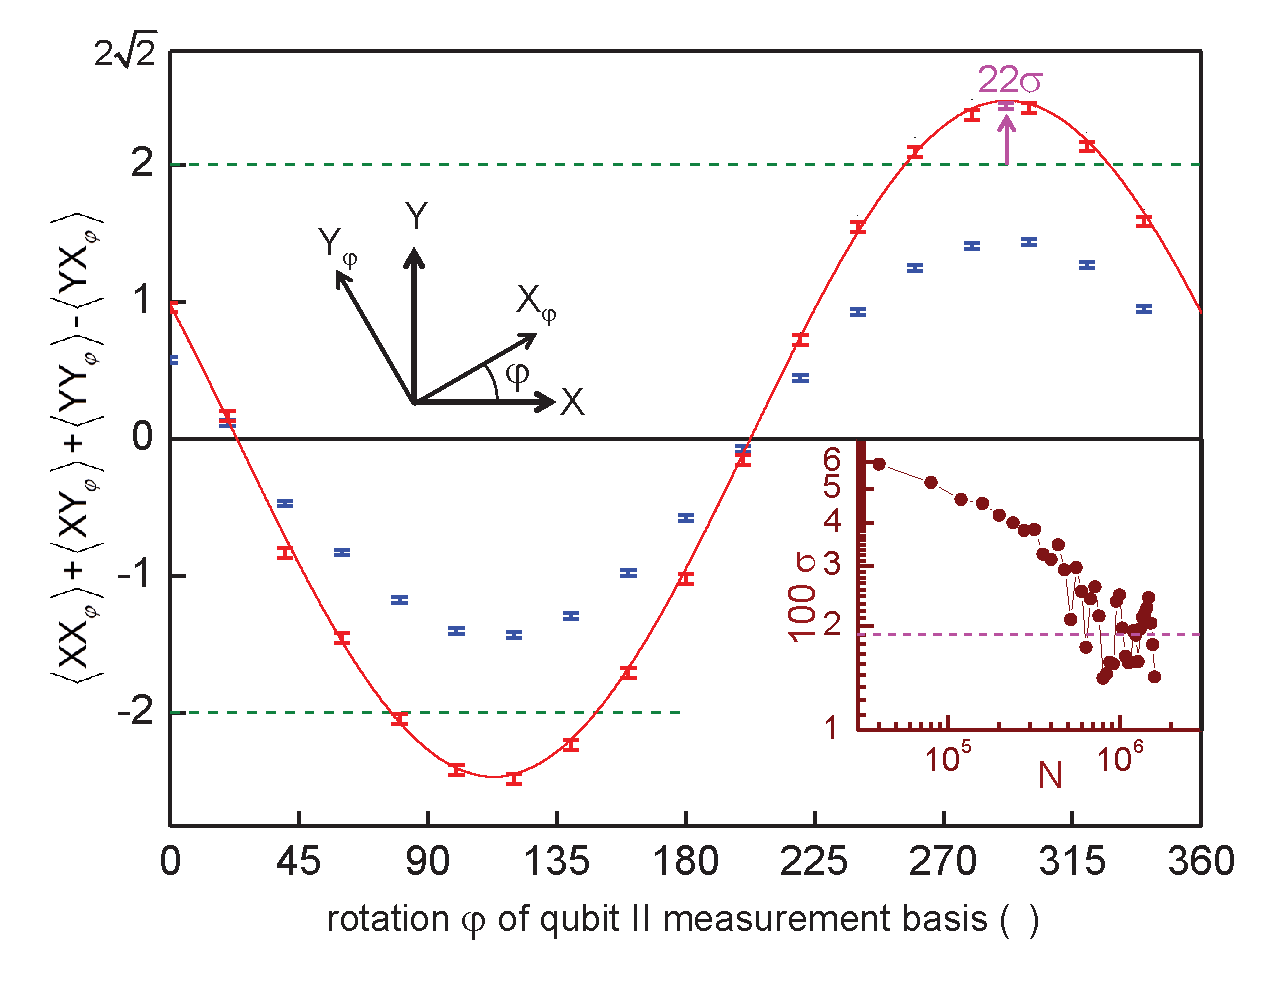
\includegraphics[width=0.8\textwidth]{./material/papers/iswap/figures/chsh}
	\caption[]{Value of the $\bracket{\mathrm{CHSH}}$ operator measured for an ensemble of identically prepared Bell states $1/\sqrt{2}(\ket{01}+e^{-i\varphi}\ket{10})$, plotted as a function of the rotation $\phi$ of the measurement basis. Blue markers correspond to raw measurement data, red markers to data corrected for readout errors. The solid line represents the best fit to the theory. The inset shows the standard deviation $\sigma$ of the maximum value of the $\bracket{\mathrm{CHSH}}$ operator as a function of the sample size. For large samples, $\sigma$ is limited by experimental drift of the measurement basis.}
	\label{fig:chsh}
\end{figure}

\subsubsection{Errors} 

Besides obvious readout errors, the main source of errors in our experiment is drift of the measurement equipment. Most importantly, the phase of the arbitrary waveform generator (AWG) can drift in respect to the phases of the microwave sources, thereby changing the effective phase of the measurement basis of the CHSH operator. Fig. \ref{fig:chsh_drift} illustrates the effect of this drift on the phase of the generated Bell state. Shown is the phase of the state $\ket{\phi}$ as given by eq. (\ref{eq:chsh_state}) extracted from a full CHSH data set as shown in fig. \ref{fig:chsh}. When repeating this measurement over a long time period, oscillations of the phase $\varphi$ with an amplitude of $\approx 40^\circ$ can be observed. This amplitude can be explained by a time shift of the AWG waveform driving the microwave sources of the order of $200\;\mathrm{ps}$, which has indeed been observed experimentally.

\begin{SCfigure}[1.0][hb!]
	\centering
	\includegraphics[width=9cm]{"./data/ct5/2011_03_17 - chsh/chsh_drift"}
	\caption[]{Phase $\varphi$ of an experimentally generated Bell state as a function of time. The phase exhibits oscillatory drift of the order of $\approx 40^\circ$ being caused by a time offset drift of the AWG.}
	\label{fig:chsh_drift}
\end{SCfigure}


\subsection{Measuring the Evolution of an Entangled Qubit States}

\begin{figure}[ht!]
   \centering
	 \includegraphics[width=1.\textwidth]{"./data/ct5/film of swap/pauli_set_vs_time_with_simulation"}
	 \caption[test]{Measured Pauli operators $\sigma_i \otimes \sigma_j$ with $i,j \in \{X,Y,Z,I\}$ as a function of the interaction time. Shown are the 6 single-qubit operators as well as the 9 two-qubit correlation operators. The dashed line represents a master-equation simulation of the experiment.}
	 \label{fig:swap_pauli_set_vs_time_with_simulation}
\end{figure}

Using quantum state tomography, we can repeat the swapping experiment described in section \ref{section:creation_of_entanglement} and reconstruct the full experimental density matrix of our system at many different times during the swap sequence. Like this we can follow the evolution of the quantum state during the course of the swap. Fig. \ref{fig:swap_pauli_set_vs_time_with_simulation} shows the result of such an experiment. We plot the measured values of all Pauli operators as a function of the swapping time between the qubits. The red and green curves correspond to the single-qubit Pauli operators $\sigma^I_{X,Y,Z}\otimes \mathrm{I}$ and $\mathrm{I}\otimes \sigma^{II}_{X,Y,Z}$, the blue curves to the two-qubit Pauli operators $\sigma_{X,Y,Z}^I\otimes \sigma_{X,Y,Z}^{II}$. The dashed line corresponds to a master equation simulation of the swapping experiment, where the qubit coupling, relaxation and dephasing parameters are chosen in accordance with experimental values. As can be seen, the simulation agrees well with the experimental data. Deviation between data and simulation can be seen in the $\sigma_{X,Y}^I\otimes \sigma_{X,Y}^{II}$ operators and is caused by an additional phase acquired by the qubits during the swap. This phase appears due to the fact that we have to shift the frequency of the qubits to bring them in resonance, hence we acquire a dynamical phase in the frame rotating at the uncoupled qubit frequencies. In addition, experimental drift of our measurement equipment may induce an additional phase factor during the measurement, which takes several hours to complete.

\smallskip

From the measured Pauli set, we can reconstruct the density matrix of the two-qubit system at any point during the swap. This density matrices are (will be soon :) shown in the margins of this thesis book. When following the evolution of the quantum state as a function of time (by flipping the pages of the book) it can be seen that the coherence between the two qubits decreases steadily during the swapping sequence, due to relaxation and dephasing.

\section{Realizing a Two-Qubit Gate}

We have demonstrated that it is possible to create highly entangled qubit states with our processor by preparing Bell states, performing quantum state tomography and violating the Bell inequality. However, to realize a universal two-qubit quantum processor, it is necessary to implement a so-called {\it universal two-qubit gate} on our processor. In the following sections we discuss how we can realize and characterize such a gate.

\subsection{Principle}

By definition, a universal two-qubit gate together with a set of universal one-qubit gates, allows us to create any possible two-qubit quantum state \citep{barenco_elementary_1995}. In principle, there are (infinitely) many choices for possible universal two-qubit gates. In this work, we are interested mainly in the so-called $\sqrt{i\mathrm{SWAP}}$ gate, which has the representation
%
\begin{equation}
U(t)=\left(\begin{array}{cccc}
1 & 0 & 0 & 0\\
0 & 1/\sqrt{2} & i/\sqrt{2} & 0\\
0 & i/\sqrt{2} & 1/\sqrt{2} & 0\\
0 & 0 & 0 & 1\end{array}\right)_{\left\{ \left|00\right\rangle ,\left|01\right\rangle ,\left|10\right\rangle ,\left|11\right\rangle \right\} } \label{eq:sqrt_iswap_gate_main}
\end{equation}
%
We can implement this gate naturally using the swapping interaction as given by eq. (\ref{eq:swap_evolution_operator_main}) when letting the qubits evolve in resonance for a time $t_{\sqrt{i\mathrm{SWAP}}}=1/8g$, which, for our experimental value of $2g = 8.3\;\mathrm{MHz}$ corresponds to $t_{\sqrt{i\mathrm{SWAP}}}=30\;\mathrm{ns}$. 

\subsection{Experimental Implementation}

Figure \ref{fig:iswap_pulse_sequence} shows the pulse sequence that we use to realize the $\sqrt{i\mathrm{SWAP}}$ gate with our processor for an exemplary input state. In the case shown, we excite the first qubit to the state $\ket{1}$, creating an input state $\ket{10}$. We then tune in resonance the two qubits for a time $t_{\sqrt{i\mathrm{SWAP}}}$. After tuning the qubits out of resonance again, we apply two single-qubit $Z$-gates to compensate the dynamical phases acquired during the swap. Then, we optionally apply single-qubit tomography gates and finally read out the qubit state at the optimal readout working point. Using this technique we can reconstruct the density matrix of the quantum state after applying the two-qubit gate to it. Similarily, we can perform quantum state tomography on the input state to obtain its density matrix. Reconstructing the input and output density matrices for a range of different input state will then allow us to fully characterize the gate operation, as will be discussed in the next section.

\begin{figure}[ht!]
	\centering
		\includegraphics[width=0.8\textwidth]{./material/papers/iswap/figures/iswap_gate_pulse_sequence}
	\caption{Experimental pulse sequence used for implementing the two-qubit $\sqrt{i\mathrm{SWAP}}$ gate. The sequence shown for an exemplary input state $\ket{10}$ consists in exciting the first qubit to the state $\ket{1}$, bringing the qubits in resonance for a time $t=1/8g$, separating them and compensating the acquired dynamical phases by using two single-qubit $Z$-pulses. Finally, optional tomographic pulses are applied before reading out the qubit state at the optimal readout frequencies of the qubits.}
	\label{fig:iswap_pulse_sequence}
\end{figure}


\subsection{Quantum Process Tomography of the Gate}

To characterize the fidelity of our quantum gate, we perform so-called {\it quantum process tomography} \citep{poyatos_complete_1997}. This procedure allows us to fully characterize a quantum process in an open quantum system. The approach that we use in this work is called {\it standard quantum process tomography} (SQPT), however, there exist other common methods such as ancilla-assisted quantum process tomography \citep{dur_nonlocal_2001,dariano_quantum_2001,altepeter_ancilla-assisted_2003}, that we will not discuss since they are not relevant to this work.

\smallskip

In the following section, we will introduce the concept of a quantum process, explain possible parametrizations of such a process and discuss the experimental implementation of standard quantum process tomography on our two-qubit processor.

\subsubsection{Theoretical Description of a Quantum Process}

A quantum process can be described as a function $\mathcal{E} : \rho_\mathcal{H} \to \rho_\mathcal{H}$ that maps a density matrix $\rho$ defined in a Hilbert space $Q_1$ to another density matrix $\mathcal{E}(\rho)$ defined in a target Hilbert space $Q_2$ and that fulfills three axiomatic properties \cite{nielsen_quantum_2000,haroche_exploring_2006}:

\begin{axiom}
$\mathrm{tr}\left[\mathcal{E}(\rho)\right]$ is the probability that the process represented by $\mathcal{E}$ occurs, when $\rho$ is the initial state.
\end{axiom}

\begin{axiom}
$\mathcal{E}$ is a {\it convex-linear map} on the set of density matrices, that is, for probabilities $\left\{p_i\right\}$,

  \begin{equation}
	  \mathcal{E}\left(\sum\limits_i p_i \rho_i\right) = \sum\limits_i p_i \mathcal{E}(\rho_i)
	\end{equation}
\end{axiom}

\begin{axiom}
$\mathcal{E}$ is a {\it completely-positive} map. That is, if $\mathcal{E}$  maps density operators of system $Q_1$ to density operators of system $Q_2$, then $\mathcal{E}(A)$ must be positive for any positive operator $A$. Furthermore, if we introduce an extra system $R$ of arbitrary dimensionality, it must be true that $(\mathcal{I}\otimes \mathcal{E})(A)$ is positive for any positive operator $A$ on the combined system $R\otimes Q_1$, where $\mathcal{I}$ denotes the identity map on system $R$.
\end{axiom}
As shown in \cite{nielsen_quantum_2000}, any quantum process fulfilling these criteria can be written in the form

\begin{equation}
  \mathcal{E}(\rho) = \sum\limits_i E_i \rho E_i^\dagger \label{eq:process_operator_sum_representation}
\end{equation}
for some set of operators $\{ E_i \}$ which map the input Hilbert space to the output Hilbert space, and for which $\sum_i E_i^\dagger E_i \le I$. Here, the operators $E_i$ are called the {\it Kraus operators} of the quantum process. They contain the full information of the quantum process acting on $\rho$.

\smallskip

If we express the operators $E_i$ in a different operator basis $\tilde{E}_j$ such that $E_i = \sum_j a_{ij} \tilde{E}_{j}$ and insert into eq. (\ref{eq:process_operator_sum_representation}), we obtain

\begin{eqnarray}
 \mathcal{E}(\rho) & = & \sum\limits_i \sum\limits_j a_{ij} \tilde{E}_j \;\rho\; \sum\limits_k a_{ik}^* \tilde{E}_k^\dagger \\
& = & \sum\limits_{j,k}\tilde{E}_j \; \rho \; \tilde{E}_k^\dagger \sum\limits_i a_{ij} a_{ik}^* \\
& = & \sum\limits_{j,k}\tilde{E}_j \; \rho \; \tilde{E}_k^\dagger \; \chi_{jk} \label{eq:process_chi_representation}
\end{eqnarray}
where we defined $\chi_{jk} = \sum\limits_i a_{ij} a_{ik}^*$. This is the so-called $\chi$-matrix representation of the quantum process. Here, all the information on the process is contained in the matrix $\chi$, which controls the action of the now process-independent operators $\tilde{E}_i$ on the initial density matrix $\rho$.

\subsubsection{Implementation}

As said before, the goal of QPT is to obtain the coefficients of the $\chi$-matrix -- or any other complete parametrization of the process -- from a set of experimentally measured density matrices $\{\rho_i\}$ and $\{\mathcal{E}(\rho_i)\}$. Standard process tomography \citep{nielsen_quantum_2000,poyatos_complete_1997} can be implemented for our two-qubit gate by using the following procedure:

\begin{enumerate}
\item Choose a set of operators $E_i$ that forms a full basis of $\mathcal{M}: Q_1 \to Q_2$. For n-qubit process tomography we usually choose $E_{i_1,i_2 \hdots i_n} = \sigma_{i_1}\otimes \sigma_{i_2}\hdots\otimes\sigma_{i_n}$, where $\sigma_i$ are the single-qubit Pauli operators and $i\in\{I,X,Y,Z\}$. For a Hilbert space of dimension $n$, this yields $4^n-1$ operators (excluding the trivial operator $I^{\otimes n}$).
\item Choose $4^n$ pure quantum states $\ket{\phi_i}$ such that the basis $\{\ket{\phi_1}\bra{\phi_1},\hdots,\ket{\phi_{4^n}}\bra{\phi_{4^n}}\}$ spans the whole space of input density matrices $\rho$. Usually, for a n-qubit system we choose $\phi = \{\ket{0},\ket{1},(\ket{0}+\ket{1})/\sqrt{2},(\ket{0}+i\ket{1})/\sqrt{2}\}^{\otimes n}$, where $^{\otimes n}$ denotes the n-dimensional Kronecker product of all possible permutations.
\item For each of the $\ket{\phi_i}$, determine $\mathcal{E}(\ket{\phi_i}\bra{\phi_i})$ by quantum state tomography. Usually we also determine $\ket{\phi_i}\bra{\phi_i}$ experimentally since the preparation of this state already entails small preparation errors that should be taken into account when performing quantum process tomography. 
\end{enumerate}

After having obtained the $\rho_i$ and $\mathcal{E}(\rho_i)$ one obtains the $\chi$-matrix by writing $\mathcal{E}(\rho_i) = \sum_j \lambda_{ij} \tilde{\rho}_j$, with some arbitrary basis $\tilde{\rho}_j$ and
letting $\tilde{E}_m \tilde{\rho}_j \tilde{E}_n^\dagger = \sum_k \beta_{jk}^{mn}\tilde{\rho}_k$. We can then insert into eq. (\ref{eq:process_chi_representation}) and obtain
\begin{eqnarray}
\sum\limits_k \lambda_{ik} \tilde{\rho}_k & = & \sum\limits_{m,n} \chi_{mn} \sum\limits_k \beta_{ik}^{mn} \tilde{\rho}_k  
\end{eqnarray}
This directly yields $\lambda_{ik} = \sum_{m,n}\beta_{ik}^{mn}\; \chi_{mn}$, which, by linear inversion,  gives $\chi$. Hence, we can fully characterize a quantum process acting on an $n$-dimensional Hilbert space by measuring $2\cdot 4^n$ experimental density matrices (or $4^n$ when assuming that no errors occur during the preparation of the input states, which thereby are known).

\smallskip

Similar to quantum state tomography, experimental errors occurring during quantum process tomography can produce a set of process parameters $\chi$ that are {\it non-physical} in the sense that the resulting quantum process does not obey the three axioms stated above. We can resolve this problem by rendering the obtained $\chi$ matrix physical by a standard mathematical procedure. When doing this, we usually choose the  physical $\chi_{ph}$ matrix that has the smallest distance $d=\|\chi-\chi_{ph}\|$.

\subsubsection{From the $\chi$ matrix to the Kraus representation}

To go back from the $\chi$-matrix representation of the quantum process to the Kraus form we write each process-independent operator $\tilde{E}_i$ as a sum of all the Kraus operators $E_l$, such that
%
\begin{equation}
	\tilde{E}_i = \sum\limits_l a_{il}\; E_l
\end{equation}
%
Inserting this into eq. (\ref{eq:process_chi_representation}) we obtain
%
\begin{eqnarray}
\begin{mathcal}E\end{mathcal}(\rho) & = & \sum\limits_{j,k}\chi_{jk}\sum\limits_{l,m} a_{jl}a_{km}^* E_l \rho E_m^\dagger   \label{eq:process_chi_transformed} \\
& = & \sum\limits_i E_i \rho E^\dagger_i
\end{eqnarray}
%
We find hence that $\sum\limits_{j,k} \chi_{jk}a_{jl}a_{km}^* = \delta_l^m$, or, written in matrix form $A\chi A^\dagger = \mathrm{I}$. This identity is true for $A$ being the matrix of eigenvectors of $\chi$, multiplied by the square root of the corresponding matrix of eigenvalues. It is thus easy to obtain the Kraus representation of the quantum process by diagonalizing the Hermitian matrix $\chi$.

\smallskip

The Kraus operator form of the quantum process is useful since it allows us to easily visualize the different operators acting on the density matrix $\rho$. By ordering the Kraus operators in function of their associated eigenvalues we can easily visualize the different unitary and non-unitary processes acting together on the density matrix $\rho$.

\subsubsection{Experimental Results: Input/Output Matrices And $\chi$-Matrix}

\begin{figure}[p]
	\centering
		\includegraphics[width=1.0\textwidth]{"./data/ct5/2011_04_21 - grover and tomo/good_data/process -matrices 1"}
	\caption{The experimental input-output density matrices of the quantum process tomography of the $\sqrt{i\mathrm{SWAP}}$ gate. Shown are the measured density matrices of 16 different input states and the corresponding output matrices with their state fidelities. The ideal matrices are overlaid in black. (part I/II)}
	\label{fig:process_matrices_1}
\end{figure}

\begin{figure}[p]
	\centering
		\includegraphics[width=1\textwidth]{"./data/ct5/2011_04_21 - grover and tomo/good_data/process -matrices 2"}
	\caption{The experimental input-output density matrices of the quantum process tomography of the $\sqrt{i\mathrm{SWAP}}$ gate. Shown are the measured density matrices of 16 different input states and the corresponding output matrices with their state fidelities. The ideal matrices are overlaid in black. (part II/II)}
	\label{fig:process_matrices_1}
\end{figure}

We perform standard process tomography of our two-qubit gate by following the procedure outlined in the last sections. Figs. \ref{fig:process_matrices_1} and \ref{fig:process_matrices_1} summarize the experimentally determined input-output density matrices, measured for our two-qubit $\sqrt{i\mathrm{SWAP}}$ quantum gate. We show pairs of corresponding input and output states together, containing both the reconstructed experimental density matrices as well as the ideal density matrices. The ideal input states are annotated below the corresponding density matrices. Above each matrix we show the trace fidelity between it and the ideal quantum state. A total of 16 input/output pairs has been measured, corresponding to a complete set of states necessary to fully characterize the quantum process of our gate operation.

\smallskip

\begin{figure}[ht!]
	\centering
		\includegraphics[width=1.\textwidth]{./material/papers/iswap/figures/chi_matrix_and_error_process}
	\caption{The reconstructed $\chi$ matrix of our implementation of the $\sqrt{i\mathrm{SWAP}}$ quantum gate. a) shows the lower half of the Hermitian matrix is shown. b) shows the product $\tilde{\chi}=\chi\cdot\chi_{id}^{-1}$ of the measured $\chi$ matrix and the ideal process matrix $\chi_{id}$. The colored arrows connecting different elements of $\tilde{\chi}$ indicate unitary and non-unitary error processes to which the corresponding matrix elements can be associated.}
	\label{fig:chi_matrix_and_errors}
\end{figure}

From these input/output matrices, we can easily calculate the $\chi$ matrix of the quantum process by the method described above. The resulting matrix is shown in fig. \ref{fig:chi_matrix_and_errors}. There, we show the experimentally obtained $\chi$ matrix of our $\sqrt{i\mathrm{SWAP}}$ gate as well as the error process defined as $\tilde{\chi} = \chi\cdot\chi_{id}$, where $\chi_{id}$ corresponds to the ideal gate process. $\chi_{id}$ is as well shown as black outlines overlaid to the measured $\chi$ matrix. The arrows connecting different parts of the $\tilde{\chi}$ matrix group several unitary and non-unitary error processes that can be attributed to the individual elements.

\subsection{Gate Fidelity}

After having obtained the experimental $\chi$ matrix, it is trivial to calculate the process fidelity, which is defined as $F=\mathrm{Tr}\{\chi_{id}\cdot\chi\}$, where $\chi_{id}$ corresponds to the ideal quantum process. For our experimental process matrix, it is given as $F=0.9$. The fidelity can be roughly compared to the output state fidelity averaged over the whole set of possible input density matrices.

\subsection{Gate Error Analysis}

We treat two classes of errors in our analysis: Unitary and non-unitary gate errors as well as tomography errors. The former are associated to errors in the quantum process itself, whereas the latter are caused by unitary and non-unitary errors during quantum state tomography.

\smallskip

\subsubsection{Tomographic Errors} \label{section:tomographic_errors}

Tomographic errors are removed from the process map of our $\sqrt{iSWAP}$
gate using the following method: The measured Pauli sets corresponding
to the sixteen input states are first fitted by a model including
errors both in the preparation of the state (index $prep$) and in
the tomographic pulses (index $tomo$). The errors included are angular
errors $\varepsilon_{\mathrm{I,II}}^{\mathrm{prep}}$ on the nominal
$\pi$ rotations around $X_{\mathrm{I,II}}$, $\eta_{\mathrm{I,II}}^{\mathrm{prep,tomo}}$and
$\delta_{\mathrm{I,II}}^{\mathrm{prep,tomo}}$ on the nominal $\pi/2$
rotations around $X_{\mathrm{I,II}}$ and $Y_{\mathrm{I,II}}$, a
possible departure $\xi_{\mathrm{I,II}}$ from orthogonality of $\left(\overrightarrow{X_{\mathrm{I}}},\overrightarrow{Y_{\mathrm{I}}}\right)$
and $\left(\overrightarrow{X_{\mathrm{II}}},\overrightarrow{Y_{\mathrm{II}}}\right)$,
and a possible rotation $\mu_{\mathrm{I,II}}$ of the tomographic
$XY$ frame with respect to the preparation one. The rotation operators
used for preparing the states and doing their tomography are thus
given by

\[
\begin{array}{c}
X_{\mathrm{I,II}}^{\mathrm{prep}}(\pi)=e^{-\mathrm{i}\left(\pi+\varepsilon_{\mathrm{I,II}}^{\mathrm{prep}}\right)\sigma_{\mathrm{x}}^{\mathrm{I,II}}/2},\\
X_{\mathrm{I,II}}^{\mathrm{prep}}(-\pi/2)=e^{+\mathrm{i}\left(\pi/2+\eta_{\mathrm{I,II}}^{\mathrm{prep}}\right)\sigma_{\mathrm{x}}^{\mathrm{I,II}}/2},\\
Y_{\mathrm{I,II}}^{\mathrm{prep}}(\pi/2)=e^{-\mathrm{i}\left(\pi/2+\delta_{\mathrm{I,II}}^{\mathrm{prep}}\right)\left[\mathrm{cos}\left(\xi_{\mathrm{I,II}}\right)\sigma_{\mathrm{y}}^{\mathrm{I,II}}\mathrm{-sin}\left(\xi_{\mathrm{I,II}}\right)\sigma_{\mathrm{x}}^{\mathrm{I,II}}\right]/2},\\
X_{\mathrm{I,II}}^{\mathrm{tomo}}(\pi/2)=e^{-\mathrm{i}\left(\pi/2+\eta_{\mathrm{I,II}}^{\mathrm{tomo}}\right)\left[\mathrm{\mathrm{sin}\left(\mu_{I,II}\right)\sigma_{x}^{I,II}+cos}\left(\mu_{\mathrm{I,II}}\right)\sigma_{\mathrm{y}}^{\mathrm{I,II}}\right]/2},\\
Y_{\mathrm{I,II}}^{\mathrm{tomo}}(-\pi/2)=e^{+\mathrm{i}\left(\pi/2+\delta_{\mathrm{I,II}}^{\mathrm{tomo}}\right)\left[\mathrm{cos}\left(\mu_{\mathrm{I,II}}+\xi_{\mathrm{I,II}}\right)\sigma_{\mathrm{y}}^{\mathrm{I,II}}\mathrm{-sin}\left(\mu_{\mathrm{I,II}}+\xi_{\mathrm{I,II}}\right)\sigma_{x}^{\mathrm{I,II}}\right]/2}.\end{array}\]
The sixteen input states are then $\{ \rho_{\mathrm{in}}^{\mathrm{e}}=U\left|0\right\rangle \left\langle 0\right|U^{\dagger}\} $
with 
%
\begin{equation}
\{ U\} =\{I_{\mathrm{I}}, X_{\mathrm{I}}^{\mathrm{prep}}(\pi), Y_{\mathrm{I}}^{\mathrm{prep}}(\pi/2),X_{\mathrm{I}}^{\mathrm{prep}}(-\pi/2)\}\otimes\{I_{\mathrm{II}},X_{\mathrm{II}}^{\mathrm{prep}}(\pi),Y_{\mathrm{II}}^{\mathrm{prep}}(\pi/2),X_{\mathrm{II}}^{\mathrm{prep}}(-\pi/2)\},
\end{equation}
%
and each input state yields a Pauli set $\left\{ \left\langle P_{\mathrm{k}}^{\mathrm{e}}\right\rangle =Tr\left(\rho_{\mathrm{in}}^{\mathrm{e}}P_{\mathrm{k}}^{\mathrm{e}}\right)\right\} $
with $\left\{ P_{\mathrm{k}}^{\mathrm{e}}\right\} =\{I_{\mathrm{I}},X_{\mathrm{I}}^{\mathrm{e}},Y_{\mathrm{I}}^{\mathrm{e}},Z_{\mathrm{I}}\}\otimes\{I_{\mathrm{II}},X_{\mathrm{II}}^{\mathrm{e}},Y_{\mathrm{II}}^{\mathrm{e}},Z_{\mathrm{II}}\}$,
$X^{\mathrm{e}}=Y^{\mathrm{tomo}}(-\pi/2)^{\dagger}\sigma_{z}Y^{\mathrm{tomo}}(-\pi/2)$,
and $Y^{\mathrm{e}}=X^{\mathrm{tomo}}(\pi/2)^{\dagger}\sigma_{\mathrm{z}}X^{\mathrm{tomo}}(\pi/2)$.
The best fit to the modeled $\left\{ \left\langle P_{k}^{e}\right\rangle \right\} $
set to the measured input Pauli sets yields $\varepsilon_{\mathrm{I}}^{\mathrm{prep}}=-1\text{\textdegree}$,
$\varepsilon_{\mathrm{II}}^{\mathrm{prep}}=-3\text{\textdegree}$,
$\eta_{\mathrm{I}}^{\mathrm{prep}}=3\text{\textdegree}$, $\mathrm{\eta}_{\mathrm{II}}^{\mathrm{prep}}=4\text{\textdegree}$,
$\delta_{\mathrm{I}}^{\mathrm{prep}}=-6\text{\textdegree}$, $\delta_{\mathrm{II}}^{\mathrm{prep}}=-3\text{\textdegree}$,
$\eta_{\mathrm{I}}^{\mathrm{tomo}}=-6\text{\textdegree}$, $\eta_{\mathrm{II}}^{\mathrm{tomo}}=-4\text{\textdegree}$,
$\lambda_{\mathrm{I}}^{t\mathrm{omo}}=12\text{\textdegree}$, $\lambda_{\mathrm{II}}^{\mathrm{tomo}}=5\text{\textdegree}$,
$\xi_{\mathrm{I}}=1\text{\textdegree}$, $\xi_{\mathrm{II}}=-2\text{\textdegree}$,
and $\mu_{\mathrm{I}}=\mu_{\mathrm{II}}=-11\text{\textdegree}$.

Knowing the tomographic errors and thus $\left\{ \left\langle P_{\mathrm{k}}^{\mathrm{e}}\right\rangle \right\} $,
we then invert the linear relation $\left\{ \left\langle P_{\mathrm{k}}^{\mathrm{e}}\right\rangle =Tr\left(\rho P_{\mathrm{k}}^{\mathrm{e}}\right)\right\} $
to find the $16\times16$ matrix $B$ that links the vector $\overrightarrow{\left\langle P_{\mathrm{k}}^{\mathrm{e}}\right\rangle }$
to the columnized density matrix $\overrightarrow{\rho}$, i.e. $\overrightarrow{\rho}=B.\overrightarrow{\left\langle P_{\mathrm{k}}^{\mathrm{e}}\right\rangle }$.
The matrix $B$ is finally applied to the measured sixteen input and
sixteen output Pauli sets to find the sixteen $(\rho_{\mathrm{in},},\rho_{\mathrm{out}})_{\mathrm{k}}$
couples to be used for calculating the gate map.

\subsubsection{Unitary and Non-Unitary Gate Errors}

After having eliminated the tomography errors, only gate errors remain. These can be unitary or non-unitary errors occuring during the quantum process. We characterize both of these errors by fitting the experimental $\chi$ matrix to a master equation model of the quantum process which includes unitary (a frequency offset when performing the swapping interaction and phase errors in the compensating $Z$ pulses applied after the swap) and non-unitary (qubit relaxation and dephasing during the whole process). Typically, the relaxation and dephasing rates employed in the simulation are chosen in accordance with experimentally measured $T_1$ and $T_2$ times (taking into account possible renormalizations of these coefficients). On the other side, the unitary error parameters are used as fitting parameters to maximize the fidelity between the experimentally measured process matrix $\chi$ and the simulated one $\chi_{sim}$. Using this technique, we can calculate an error budget of the quantum process that quantifies the contributions of individual error sources. For our process, we find a total gate error of $10 \%$, where we can attribute $8\%$ of the errors to relaxation and decoherence during the process and $2\%$ to unitary gate errors. In principle, after having characterized the unitary gate errors occurring during the process we could, in theory, compensate them in our experiment. However, due to fast drift of the qubit parameters during the experiment we usually do not perform this kind of optimal qubit control to our gate. Under certain circumstances, the effect of non-unitary errors can also be compensated or alleviated by adding or modifying the unitary gate sequence during the quantum process (see e.g. \citep{lange_universal_2010}). However, this procedure is in general not applicable to arbitrary quantum processes and is not applicable to this work.



\chapter{Running the Grover Search Algorithm} \label{chapter:grover_algorithm}

This chapter describes an experimental implementation of the so-called {\it Grover search algorithm} with our two-qubit quantum processor. The first section provides a short introduction of the algorithm and motivates the interest in realizing it. The following sections then discuss the details of its experimental realization. We show the results that we obtained and compare the algorithm fidelity and efficiency to that of an equivalent, classical algorithm. Finally, we analyze all relevant unitary and non-unitary error sources relevant to our experiment and provide a quantitative error model of our implementation of the algorithm.

\section{Introduction \& Motivation}

Search algorithms are of great importance in many domains of mathematics and computer science. One such search problem that often arises and which will be discussed in the following sections can be formulated in simple terms as follows:

\smallskip

Assume that we have a search space $\begin{mathcal}S\end{mathcal}$ that consists of a finite number $N$ of states $s \in \begin{mathcal}S\end{mathcal}$. The solution to our search problem corresponds to a subset of $M$ states of the search space $\begin{mathcal}T\end{mathcal} \subset \begin{mathcal}S\end{mathcal}$. We can then define a search function $\Or(s):\begin{mathcal}S\end{mathcal}\to \{0,1\}$ that discriminates between states that solve the search problem and states that don't, such that $\Or(s) = 1$ for $s \in \begin{mathcal}T\end{mathcal}$ and $\Or(s) = 0$ otherwise. In accordance with the general convention in the literature on the Grover search algorithm, we will  often refer to this search function as the {\it Oracle function} or (in a quantum-mechanical context) as the {\it Oracle operator}.

\smallskip

Using this definition of the search problem, the goal of a search algorithm is to find all states $t\in\begin{mathcal}S\end{mathcal}$ for which $\Or(t) = 1$. In the following, for the sake of simplicity we assume that the solution set $\begin{mathcal}T\end{mathcal}$ contains only one single state $t$. This special case can be generalized to cases where more than one solution to the search problem exists (see e.g. \cite{nielsen_quantum_2000,mermin_quantum_2007} for a detailed review)

\smallskip

The first step in order to solve a search problem of the kind described above using classical or quantum computation is to map the problem to a form suitable for solution by a digital (quantum) computer. For this, we first number and encode the $N$ input states $i \in \begin{mathcal}S\end{mathcal}$ in binary form as $i=(b^i_l,\hdots,b^i_0)_B$, where $l$ is the length of the binary register able to hold all $N$ input states. With this definition, it is then trivial to find a mathematical representation of $\Or$ that operates on a binary input register. 

\smallskip

Using these assumptions and definitions, it can be shown that the most efficient classical search algorithm for solving the search problem above will use $\begin{mathcal}O\end{mathcal}(N)$ calls of the function $\Or$ to find the solution of the search problem. If assuming that calling $\Or$ is much more ``expensive'' in time or resources than any other operation, $\begin{mathcal}O\end{mathcal}(N)$ will then also correspond to the overall computational efficiency of the algorithm.

\smallskip

Amazingly, in 1997, Lov Grover found a quantum algorithm that could solve this search problem with only $\begin{mathcal}O\end{mathcal}(\sqrt{N})$ calls to the function $\Or$ \citep{Grover_Quantum_1997}. His algorithm achieves this by repeatedly calling a quantum-mechanical implementation of the function $\Or$, starting from a highly superposed qubit register $\sum\limits_i^N \ket{i}$ and applying a special operator to the resulting output state afterwards. The individual steps of his algorithm are given as follows:

\begin{enumerate}
 \item Initialize a qubit register to the state $\ket{\psi} = \ket{0}$ (corresponding to a binary input state $\ket{0000\hdots0_B}$)
 \item Apply the generalized Hadamard operation to the qubit register, producing a fully superposed quantum state $$\ket{\psi} = \frac{1}{\sqrt{N}}\sum\limits_{i=0}^{N-1} \ket{i}$$
 \item Repeat the following sequence $\begin{mathcal}O\end{mathcal}(\sqrt{N})$ times:
 \subitem a) Apply the {\it Oracle operator} $\ket{i}\to (-1)^{\Or(i)}\ket{i}$.
 \subitem b) Apply the so-called {\it diffusion operator} $\ket{i} \to -\ket{i}+\frac{2}{N}\sum\limits_{j=0}^{N-1}\ket{j}$.
	\item Measure the state of the quantum register in the computational basis $\ket{i}$.
\end{enumerate}

Note that for the description above we have enumerated the states of the qubit register from $\ket{0}$ to $\ket{N-1}$. The Grover algorithm makes use of quantum parallelism to solve the search problem $\begin{mathcal}O\end{mathcal}(\sqrt{N})$ times faster than the most efficient classical algorithm. To understand better the strategy it uses, the different steps of the algorithm can be rephrased in the following, more general way:

\begin{itemize}
\item First, the algorithm creates a fully superposed quantum state which contains all possible solutions to the search problem at once. The amplitudes and phases of each individual state are all equal in the beginning.
\item Then, it applies the Oracle operator to this superposed state. The effect of the Oracle is to turn the phase of the state $t$ for which $\Or(t)=1$ by an angle $\pi$. As will be shown later, such an Oracle operator can be implemented in a straightforward way for any classical search function.
\item In the next step, it applies a diffusion operator to the quantum state which transfers a fraction of the amplitude from states with zero phase to the states with $\pi$ phase, increasing thus the amplitude of the latter. In this process, the phases of all states get also turned back to zero, allowing the algorithm to repeat the sequence above.
\item Repeating these two operations increases each time the amplitude of the states that correspond to a solution of the search problem until the amplitudes of all the other states vanish. After that point, the process reverses and the amplitude is transferred back to the original states. It is therefore crucial to stop the repetition sequence given above after the right number of iterations.
\end{itemize}

By implementing the search function as a quantum operator acting on a superposition, the Grover algorithm is able to somehow evaluate it in one single call for all possible input states. This so-called {\it quantum parallelism} provides the basis for the speed-up of the search in comparison to a classical algorithm. However, being able to encode the result of the search function in the phase of a multi-qubit state does not directly translate to a speed advantage since it is usually very hard to extract this phase information from the quantum state. Indeed, to extract the values of all phases from an $N$-qubit state, it would be necessary to perform $\begin{mathcal}O(2^N)\end{mathcal}$ measurements on an ensemble of such identically prepared quantum states. However, extracting the amplitudes from such a state takes only $\begin{mathcal}O\end{mathcal}(N)$ measurements, that in addition can usually be carried out in parallel. It is for this reason that the Grover algorithm uses an operator that transforms the information encoded in the phases of the qubits to an information encoded in their amplitude. However, since the conversion between phase to amplitude information through the application of an unitary operator is limited by certain physical constraints, the algorithm needs to repeat the encode-and-transfer sequence described above $\begin{mathcal}O(\sqrt{N})\end{mathcal}$ times. \cite{lloyd_quantum_1999,meyer_sophisticated_2000,lanyon_experimental_2008,ahn_information_2000,ding_review_2007,linden_good_2001,braunstein_speed-up_2002}

\smallskip

To analyze further the constraints and principles of the algorithm, we will discuss a more detailed derivation of it starting from the Schrödinger equation and we will also explain what limits the efficiency of the phase-to-amplitude conversion in the algorithm.

\subsection{Deriving the Grover Algorithm from Schrödinger's Equation}


An interesting derivation of the Grover algorithm starting from Schrödinger's equation has been detailed by Grover himself in a seminal paper \citep{grover_schrodingers_2001} and shall be briefly rediscussed here since it sheds light on the basic principles on which the algorithm is based. The derivation begins by considering a quantum system governed by Schrödinger's equation, which can be written as (setting $\hbar = 1$ for better readability)
%
\begin{equation}
-i\frac{\partial}{\partial t}\psi(x,t) = \frac{\partial^2}{\partial x^2}\psi(x,t)-V(x)\psi(x,t) \label{eq:grover_derivation}
\end{equation}
%

\begin{wrapfigure}{r}{6cm}
\vspace{-1cm}
\includegraphics[width=5.2cm]{"./material/papers/grover/grover_derivation_schroedinger"}
\caption{Wave function $\psi(x)$ and potential $V(x)$ defined on a grid of points $x_1,\hdots,x_N$. A minimum of the potential can encode a search value $x_i$.}
\label{fig:GroverDerivationSchroedinger}
\end{wrapfigure}


Here $\psi(x,t)$ describes the wave-function and $V$ is a time-independent potential. Let us assume that the potential $V(x)$ is shaped as in fig. \ref{fig:GroverDerivationSchroedinger}, i.e. possessing a global minimum of energy. When one initializes the system to a state $\psi_0(x,t_0)$ and lets it evolve for a given time, $\psi(x,t)$ will be attracted by the minimum of potential energy and ``fall into it'' much like a classical particle in such a potential would\footnote{Of course, since there is no dissipation, the state will not come to rest at the minimum point of energy but rather oscillate around it conserving its total potential and kinetic energy.}. We might thus ask if we can encode the solution to a search problem as a point of minimum energy $x_0$ of a potential $V(x)$, take an initial state $\psi_0(x,t_0)$ and let it evolve into a state that has a high probability around $x_0$, thereby solving the search problem. To answer this question, it is first necessary to discretize the wave function $\psi(x,t)$ such that it can represent the search problem stated in the last section, and which is defined over a finite number of states. In the most simple case, we can use a regular grid of points $x_i$ with a spacing $\Delta x$ for this, as shown in fig. \ref{fig:GroverDerivationSchroedinger}b. Discretizing the time evolution of eq. \ref{eq:grover_derivation} in steps $\Delta t$ as well and defining $\epsilon = \Delta t/\Delta x^2$, we obtain a new equation of the form
%
\begin{equation}
-\frac{\psi_i^{t+\Delta t}-\psi_x^{t}}{\Delta t} = \frac{\psi_{i+1}^t+\psi_{i-1}^t-2\psi_x^t}{\Delta x^2} -V(x_i)\psi_i^t
\end{equation}
%
where we have written $\psi(x_i,t)=\psi_i^t$. For a circular grid with $N$ points we can write this equation in matrix form as
%
\begin{equation}
\vec{\psi}^{t+\Delta t} = S^{\Delta t}  \cdot \vec{\psi}^t
\end{equation}
%
with $S$ being a state transition matrix of the form
%
\begin{equation}
S^{\Delta t} = \left(
	\begin{array}{ccccc}
		1-2i\epsilon-iV(x_1)\Delta t & i\epsilon & 0 & \hdots &  i\epsilon \\
		i \epsilon & 1-2i\epsilon -iV(x_2)\Delta t & i\epsilon & \hdots & 0 \\
		0 & i\epsilon & \ddots & & \vdots \\
		\vdots & & & \ddots  & \vdots \\
		i \epsilon & 0 & \hdots & i\epsilon & 1 - 2i\epsilon -iV(x_N)\Delta t
	\end{array}
 \right) \label{eq:grover_iteration_matrix}
\end{equation}
%
For infinitesimal times $\Delta t$ we can separate the effect of the potential $V(x)$ on the wave function from the spatial dispersion $\propto i\epsilon$ by writing $S^{\Delta t} \approx D\cdot R$ with 
%
\begin{eqnarray}
D & = & \left( 
		\begin{array}{cccccc}
		1-2i \epsilon & i\epsilon & 0 & 0 & \hdots & i\epsilon \\
		i \epsilon & 1 - 2i \epsilon & i \epsilon & 0 & \hdots & 0 \\
		\hdots & \ddots & & & & \vdots \\
		i \epsilon & 0 & 0 &  \hdots & i\epsilon & 1-2i \epsilon \\
		\end{array}
	\right)
\end{eqnarray}
%
and 
%
\begin{eqnarray}
R & = & \left( \begin{array}{ccccc}
	e^{-i V(x_1) \Delta t} & 0 & \hdots & 0 \\
	0 & e^{-i V (x_2) \Delta t} & \hdots & 0 \\
	0 & \hdots & & 0 & e^{-i V (x_N) \Delta t} \\
	\end{array}
	\right)
\end{eqnarray}
%
This approximation is correct to order $\begin{mathcal}O\end{mathcal}(\epsilon)$ up to an irrelevant renormalization factor. Now, we can repeatedly apply the matrix product $D\cdot R$ to the wave function to obtain its state after a given finite time $t$ by writing
%
\begin{equation}
\vec{\psi}^{t_0+t} = \left(\prod\limits_{i = 1}^{t/\Delta t} D\cdot R\right)\cdot \vec{\psi}^{t} \label{eq:trotter_evolution}
\end{equation}
%
This technique of splitting up the full evolution operator into a product of two or more non-commuting operators that are applied repeatedly to the wave function to obtain its state after a finite time is sometimes referred to as {\it Trotterization} -- in reference to the so-called {\it Lie-Trotter formula} on which it is based -- and on which digital quantum simulation relies\citep{lloyd_universal_1996,lanyon_universal_2011}.

\smallskip

As can be seen in eq. (\ref{eq:trotter_evolution}), the evolution of the wave function at infinitesimal times is governed by two processes: The interaction with the potential $V$ and a diffusion process that mixes different spatial parts of the wave function with each other. The operator $D$ resembles a Markov diffusion process since each row and column of the matrix sums up to unity, whereas $R$ changes the phase of each element of the wave function as a function of the local potential seen by it. If we apply $R$ to a fully superposed initial state of the form $\psi_i = 1$ (omitting the normalization factor for simplicity) and assume that $V_i = 0$ for $i \ne j$ and $V_j \Delta t = \pi/2$ (the potential thus encoding a search function with $\Or(j)=1$ and $\Or(i)=0$ for $i\ne j$), the element $\psi_j$ will get turned according to $\psi_j \to i\psi_j $, whereas all other elements $\psi_i$ will remain unchanged. Applying the operator $D$ to the resulting state will transform $\psi_j$ according to $\psi_j \to \psi_j(i+2\epsilon(1+i))$ with a corresponding amplitude $\sqrt{1+4\epsilon+\begin{mathcal}O\end{mathcal}(\epsilon^2)}$ and the adjacent states $\psi_{j\pm 1}$ according to $\psi_{j\pm 1} \to \psi_{j\pm 1}(1-\epsilon(1+i))$ with an amplitude $\sqrt{1-2\epsilon +\begin{mathcal}O\end{mathcal}(\epsilon^2)}$. Hence there is a transfer of amplitude between the state whose phase has been turned and its neighboring states. If we reset the phases of all the $\psi_i$ to zero afterwards, we can iterate the application of $D\cdot R$ until all of the amplitude has been transferred to the element $\psi_j$ which corresponds to a solution to the search problem. This is, in essence, exactly what the Grover algorithm does, the only difference being that it replaces the matrix $D$ with an unitary matrix that maximizes the amplitude transfer to the states solving the search problem, thereby speeding up the algorithm. As stated before, the efficiency with which the algorithm can transfer amplitude between different states is limited by physical constraints. In the next section, we will therefore discuss exactly what limits this efficiency and which unitary diffusion matrix one should choose to maximize it.

\subsubsection{Efficiency of Quantum Searching}

As discussed by L. Grover \citep{grover_schrodingers_2001}, it is interesting to ask what is the maximum amount of amplitude that can be transferred in a single step of the Grover search algorithm and which matrix $D$ should be chosen to maximize this transfer. To answer this question and derive the ideal diffusion matrix, we will assume first that, without loss of generality, the matrix $R$ which encodes the value of the search function $\Or$ in the quantum state of the qubit register can be written as
%
\begin{eqnarray}
R & = & \begin{mathrm}I\end{mathrm}-2\sum\limits_{j=0}^{N-1} \Or(j)\ket{j}\bra{j}. \label{eq:GroverOracleFunction}
\end{eqnarray}
%
This operator will flip the sign of all states for which $\Or(j) = 1$. Now, the next step consists in finding a diffusion or state transfer matrix which will maximize the amplitude transfer to states tagged by the Oracle operator above and which will also reset the phases of the quantum register to zero afterwards, such that we might apply the Oracle operator to the resulting state again. In the most general case, such a state transfer matrix will have the form
%
\begin{equation}
D_c = \left(	
	\begin{array}{ccccc}
		b & a & a & \hdots & a \\
		a & b & a & \hdots & a \\
		\vdots & & \ddots &  &\vdots \\
		a & & \hdots & a & b \\
	\end{array}
\right).
\end{equation}
%
Here, we assume that all non-diagonal elements of the matrix are equal, which is well justified since we have no knowledge of the structure of the search space of the problem and therefore want to treat all basis states equally during the phase-to-amplitude conversion. Furthermore, since both the initial quantum state and the Oracle operator as given by eq. (\ref{eq:GroverOracleFunction}) contain only real numbers and we demand that the quantum state after applying $D_c$ may contain only positive real numbers as well it is easy to show that $a,b$ must be real numbers. Finally, the unitarity of quantum operators demands that $D_c^\dagger D_c = \begin{mathrm}I\end{mathrm}$, which for the matrix above is equivalent to the two conditions
%
\begin{eqnarray}
 1 & = & b^2+(N-1)a^2, \\
0 & = & 2ab +(N-2)a^2.
\end{eqnarray}
%
Solving these two equations for $a,b$ yields the trivial solution $b = \pm 1$, $a = 0$ and the more interesting one $b = \pm(1-2/N)$, $a=\mp 2/N$. As can be checked easily, the solution $b = 1-2/N$, $a = 2/N$ results in a maximum amplitude transfer from states $\ket{i}$ for which $\Or(i)=0$ to states $\ket{j}$ for which $\Or(j)=1$. Thus the ideal diffusion matrix to be used in the Grover algorithm is given as
%
\begin{equation}
D = \left( \begin{array}{ccccc}
	-1+2/N & 2/N & 2/N & \hdots & 2/N \\
	2/N & -1 + 2/N & 2/N & \hdots & 2/N \\
	\vdots & & \ddots &  & \vdots \\
	2/N & 2/N & 2/N & \hdots & -1 + 2/N \\ 
	\end{array} \right). \label{eq:GroverDiffusionOperator}
\end{equation}
%
This matrix, together with an Oracle operator $R$ as given by eq. (\ref{eq:GroverOracleFunction}) will yield the maximum amplitude transfer from states not solving the search problem to states that solve it. Repeating the application of $D\cdot R$ on an initially fully superposed quantum state for $\begin{mathcal}O\end{mathcal}(\sqrt{N})$ times will transform the input state to a state containing only the solutions of the search problem.

\smallskip

For the two-qubit case, the Oracle and diffusion operators $R$ and $D$ of the previous sections are
%
\begin{eqnarray}
	R  & = & \left( \begin{array}{rrrr} (-1)^{\Or(00)} & 0 & 0 & 0 \\ 0 & (-1)^{\Or(01)} & 0 & 0 \\ 0 & 0 & (-1)^{\Or(10)} & 0 \\ 0 & 0 & 0 & (-1)^{\Or(11)} \end{array} \right), \label{eq:two_qubit_oracle_operator} \\
  D  & = & \frac{1}{2}\left( \begin{array}{rrrr} -1 & 1 & 1 & 1 \\ 1 & -1 & 1 & 1 \\ 1 & 1 & -1 & 1 \\ 1 & 1 & 1 & -1 \end{array} \right). \label{eq:two_qubit_diffusion_operator} 
\end{eqnarray}
%
Before discussing the experimental implementation of this algorithm, we will show how we can compare its computational efficiency to that of an equivalent classical algorithm in order to assess the achieved quantum speed-up.

\subsection{Comparison to Classical Algorithms}

To be able to compare the Grover algorithm as outlined here to a classical version solving the same search problem, we will now discuss another variant of the algorithm that uses an ancilla qubit to encode the result of the search function. This implementation will make it possible to devise a classical algorithm that can be directly compared to the quantum algorithm. 

\subsection{Ancilla-based Implementation of the Algorithm}

\begin{figure}[ht!]
	\centering
		\includegraphics[width=0.8\textwidth]{./material/papers/grover/different_oracle_implementations}
	\caption[]{a) Definition of the NOT logic gate used in the following diagrams. b) Ancilla-based implementations of the Oracle functions $\Or$ for two qubits. The state of the third bit get flipped if the search function $\Or(i)=1$ for the given input state $i$. c) Example of an ancilla-based search function returning a true value for the input state $00$.}
	\label{fig:GroverOracleImplementations}
\end{figure}

The implementation of the Grover search algorithm as outlined above encodes the value of the search function $\Or$ directly in the phase of the input state supplied to this function. This makes it hard to compare the algorithm to a classical search algorithm which operates on a binary input state and, in general, cannot encode the result of the search function directly in this state. It is therefore useful to formulate a version of the Grover algorithm where the Oracle function does not directly encode the tagged state in the input qubit register but rather uses an ancilla qubit to store the result of calling $\Or$. Such a representation of the algorithm, although of little practical relevance, is useful since it allows us to directly compare the quantum algorithm to a classical counterpart implemented using reversible logic gates, thus making it possible to benchmark the quantum algorithm and provide an estimation of the quantum speed-up that can be achieved.

\smallskip

Exemplary implementations of ancilla-based search functions $\Or$ implemented using reversible (quantum) gates are shown in fig. \ref{fig:GroverOracleImplementations} for the two-qubit case. There, a three-qubit Tofolli gate in combination with several single-qubit NOT gates (that can be easily implemented as single-qubit $X_{\pi}$ rotations) are used to flip the state of an ancilla-qubit conditionally on the input state of the gate. Using a similar approach, any arbitrary classical search function $\Or$ that can be implemented with a set of universal reversible logic gates (e.g. the Toffoli gate and the NOT gate) can be directly mapped to a corresponding quantum operator that works on quantum-mechanical input states and implements the classical search function.

\begin{figure}[ht!]
	\centering
		\includegraphics[width=1\textwidth]{./material/papers/grover/quantum_algorithm_full}
	\caption{Full version of an ancilla-based implementation of the two-qubit Grover search algorithm. The algorithm flips the state of a (third) control qubit for one of the four possible input states in accordance to an unknown Oracle function. It then applies a three-qubit control-phase operation of that maps $\ket{xy1}\to -\ket{xy1}$, $\ket{xy0}\to\ket{xy0}$ to encode the state of the control qubit directly in the two input qubits. Then, a diffusion operator is used to determine the state which has been tagged by the Oracle function.}
	\label{fig:GroverAlgorithmFullSchematic}
\end{figure}

\smallskip

Now, to use the Grover algorithm with such an ancilla-based quantum Oracle, it is necessary to re-encode the result of the Oracle in the qubit input state. Figure \ref{fig:GroverAlgorithmFullSchematic} shows a version of the two-qubit Grover algorithm that achieves exactly this by using a three-qubit control-control-not (CCNOT) gate $C$ of the form
%
\begin{equation}
C = \mathrm{I}^{8\otimes 8}-2\sum\limits_{ij} \ket{ij1}\bra{ij1}.
\end{equation}
%
After the re-encoding of the result, the ancilla qubit is not needed during the remainder of the algorithm but must not be read out before the algorithm terminates. A discussion of possible realizations of the ancilla-based Oracle operator can also be found in \citep{mermin_quantum_2007}.

\subsection{Comparison to a Classical Algorithm}

\begin{figure}[ht!]
	\centering
		\includegraphics[width=1.0\textwidth]{"./material/papers/grover/classical_reversible_algorithm"}
	\caption{Classical reversible implementation of a query-and-guess search algorithm on a two-bit input register. An exemplary Oracle function can be implemented using two single-bit NOT operations and a Toffoli gate. R designates the generation of a random binary value at the beginning of the algorithm. If the Oracle does not yield the correct answer, the test state is incremented. The average success probability of the algorithm is 50 \%.}
	\label{fig:GroverClassicalReversibleAlgorithm}
\end{figure}

In order to quantify the speed-up achieved by a quantum algorithm, it is necessary to define an equivalent classical algorithm to which we can compare it. Using the reversible, ancilla-based implementation of the search function that was introduced in the last section, it is straightforward to formulate a classical algorithm that solves the same problem as the Grover algorithm and then compare the number of evaluations of the search function $\Or$ of the two. In this work, we compare our quantum algorithm to two particular classical algorithms that we refer to as ``query'' and ``query-and-guess''. The query algorithm evaluates $\Or$ for $n$ states, returning the searched state if it finds it among them and returning no value at all otherwise. The query-and-guess algorithm also evaluates $\Or$ for $n$ states, but even if the searched state is not found, it returns a guess of it by e.g. picking one of the remaining states at random. A possible two-bit implementation of a classical reversible query-and-guess algorithm that evaluates $\Or$ only once is shown in fig. \ref{fig:GroverClassicalReversibleAlgorithm}, achieving a success probability of 50 \% by evaluating $\Or$ for a randomly generated two-bit input value $r$ and returning $r$ if $\Or(r)=1$ or $r+1(\mathrm{mod}\;4)$ otherwise. Allowing two or three evaluations of $\Or$ will increase the success probability to \mbox{75 \%} or \mbox{100 \%}, respectively. The success probability of an equivalent two-qubit query algorithm would be 25 \% for one evaluation of $\Or$, 50 \% for two, 75 \% for three and 100 \% for four. In general, for a search space with $N$ states, the success probabilities of the query and query-and-guess algorithms as a function of $n$ are $p_s^{q}(n)=n/N$ (for $n \le N$) and $p_s^{qg}(n)=(n+1)/N$ (for $n \le N-1$), which become equivalent for $N \to \infty$ but deviate significantly for small $N$.

\section{Experimental Implementation}

\begin{figure}[ht!]
	\centering
		\includegraphics[width=\textwidth]{./material/papers/grover/grover_algorithm}
	\caption{Schematic of our implementation of the Grover search algorithm. The algorithm consists in generating a fully superposed input state, applying the Oracle function to it and analyzing the resulting state by applying the Diffusion transform and reading out the value of the qubit register afterwards.}
	\label{fig:GroverAlgorithmSchematic}
\end{figure}

The Grover algorithm has been implemented for two and three qubits using nuclear magnetic resonance (NMR) \citep{chuang_experimental_1998,vandersypen_implementation_2000} as well as for two qubits using trapped ions \citep{brickman_implementation_2005} and recently NV centers in diamond \citep{sar_decoherence-protected_2012}. In 2009, L. DiCarlo {\it et. al.} implemented it using a superconducting two-qubit processor \citep{dicarlo_demonstration_2009} achieving $>80 \%$ output state fidelity, albeit without using a sufficiently efficient readout scheme of the qubit register and therefore not being able to demonstrate quantum speed-up. The demonstration of quantum speed-up for the Grover search algorithm using a superconducting two-qubit processor with individual-qubit readouts is one of the main goals of this thesis work.

\smallskip

We implement the compiled version of the two-qubit Grover algorithm, which encodes the result of calling the Oracle function $\Or(x)$ with an input state $x$ directly in the phase of $x$, as described above. The gate sequence of the algorithm is shown in fig. \ref{fig:GroverAlgorithmSchematic} and consists of two $i\mathrm{SWAP}$ gates and six single-qubit gates applied to an initial state $\ket{00}$. Here, the first $i\mathrm{SWAP}$ gate (which includes a $Z_{\theta_I}^I\otimes Z_{\theta_{II}}^{II}$ gate sequence to compensate the acquired phases of the qubits) together with the two single-qubit $Z_{\pm \pi/2}$ rotations implements the Oracle function $\Or(x)$ as given by eq. (\ref{eq:two_qubit_oracle_operator}), where the signs of the rotation operations determines the state which is tagged by the Oracle ($--$, $-+$, $+-$ and $++$ for $\Or_{00}$, $\Or_{01}$, $\Or_{10}$ and $\Or_{11}$, respectively). This state can be either $\ket{00}$ (corresponding to a $Z^I_{-\pi/2}\cdot Z^{II}_{-\pi/2}$ rotation), $\ket{01}$ ($Z^I_{-\pi/2}\cdot Z^{II}_{\pi/2}$), $\ket{10}$ ($Z^I_{\pi/2}\cdot Z^{II}_{-\pi/2}$) or $\ket{11}$ ($Z^I_{\pi/2}\cdot Z^{II}_{\pi/2}$). After the encoding, the second $i\mathrm{SWAP}$ operation (which also includes Z compensation pulses) together with the following $X^I_{\pi/2}\cdot X^{II}_{\pi/2}$ single-qubit operations implements the diffusion operator as given by eq. (\ref{eq:two_qubit_diffusion_operator}). The final step of the algorithm consists in reading out the two-qubit register.

\subsection{Pulse Sequence}

\begin{figure}[ht!]
	\centering
		\includegraphics[width=0.95\textwidth]{./material/papers/grover/figures/grover_algorithm_pulse_sequence}
	\caption{Pulse sequence used to realize the two-qubit Grover quantum search algorithm. First, a $Y_{\pi/2}$ pulse is applied to each qubit to produce the fully superposed state $1/2(\ket{00}+\ket{01}+\ket{10}+\ket{11})$. Then, an $i\mathrm{SWAP}$ gate is applied, followed by a $Z_{\pm \pi /2}$ gate on each qubit, which combined correspond to the application of the Oracle function. The resulting state is then analyzed using another $i\mathrm{SWAP}$ gate and two $X_{\pi/2}$ gates to extract the state tagged by the Oracle. Optionally, a $Y^{12}_{\pi}$ pulse is applied to each qubit to increase the readout fidelity.}
	\label{fig:GroverPulseSequence}
\end{figure}

\begin{figure}[hp!]
	\centering
		\includegraphics[width=0.95\textwidth]{"./data/ct5/2011_04_21 - grover and tomo/good_data/grover algorithm - summary"}
	\caption{a) Schematic of the implemented algorithm, indicating the steps at which quantum state tomography has been performed. b) Experimental (filled circles) and theoretical (black outline) density matrices at different steps of the Grover search algorithm as indicated by the dotted lines, shown for four individual runs of the algorithm corresponding to different Oracle functions tagging the state ${\ket{00}}$, ${\ket{01}}$, ${\ket{10}}$ or ${\ket{11}}$. The trace fidelity (\ref{eq:quantum_trace_fidelity}) between experimental and theoretical density matrices is indicated above each matrix.}
	\label{fig:GroverAlgorithmExperimentalResults}
\end{figure}

We implement the gate sequence described above using microwave and fast flux pulses. To minimize gate errors, we perform a series of calibration measurements before to tune-up the individual single- and two-qubit gates needed for the algorithm, as explained in chapter \ref{chapter:processor_characterization}. In addition, we run individual parts of the algorithm successively and perform quantum state tomography to characterize the state of the quantum register after each step of the algorithm, optimizing the gate operations applied to the qubit in order to maximize the fidelity of the measured states in respect to the ideal ones. However, we optimize only the state preparation and Oracle operator itself on a per-state basis, whereas the diffusion operator $D$ is optimized only once for all possible Oracles, as required for benchmarking a real quantum algorithm. cases do not optimize the  Figure \ref{fig:GroverPulseSequence} shows an experimental pulse sequence for the Grover algorithm with an Oracle operator $\Or_{00}$. Shown are the frequencies of the two qubits during the run time of the algorithm and the microwave drive and readout pulses applied to them.

\section{Results}

We now present the experimental results obtained with our implementation of the Grover algorithm: Quantum state tomography is first used to determine the register density matrices during the algorithm, and single-run results are then presented and discussed.

\subsection{State Tomography of the Quantum Register}

Figure \ref{fig:GroverAlgorithmExperimentalResults}b shows the experimentally measured density matrices of the two-qubit register when running the Grover search algorithm for the four possible Oracle functions. For each of those four cases, quantum state tomography was performed after each step of the algorithm, as indicated in fig. \ref{fig:GroverAlgorithmExperimentalResults}a. The fidelity diminishes during the algorithm due to dephasing and relaxation. The state fidelities for the final output states of the algorithm are $68\%$ for the $\Or_{00}$, $64\%$ for the $\Or_{01}$, $61\%$ for the $\Or_{10}$ and $65\%$ for the $\Or_{11}$ Oracle functions.

\subsection{Single Run Results}

\begin{figure}[ht!]
	\centering
		\includegraphics[width=1.\textwidth]{"./data/ct5/2011_04_21 - grover and tomo/good_data/grover algorithm - single run probabilities"}
		\caption{Single-run success probabilities of our implementation of the Grover search algorithm, for the four possible Oracle functions. Red bars correspond to measured values, whereas blue ones are calculated using the measured density matrices after the final step of the algorithm and the measured two-qubit readout matrix as shown in fig. \ref{fig:GroverReadoutMatrix}. Dashed lines indicate the average success probabilities of classical query and query-and-guess algorithms, for comparison.}
	\label{fig:GroverSingleShotResults}
\end{figure}

The experimental state tomographies presented above show that we can implement the Grover search algorithm with average output state fidelity of 64 \% using our two-qubit processor. However, the analysis of the two-qubit register by quantum state tomography at the end of the algorithm does not prove that we can achieve real quantum speed-up with our processor. For this, it is necessary to directly read out the state of the qubit register at the end of the algorithm {\it without} performing any kind of error correction afterwards. By looking at this ``raw'' outcome data and generating statistics over many single runs of the processor, we quantify the success rate and the fidelity of the implemented algorithm. The results of such measurements, performed for the four possible Oracle functions, are shown in fig. \ref{fig:GroverSingleShotResults}. Besides the single-run probabilities for all four Oracle functions, the diagram shows for comparison the expected outcome probabilities calculated based on the quantum state tomographies discussed above and the readout matrix of the two-qubit processor shown in fig. \ref{fig:GroverReadoutMatrix}. As can be seen, the agreement between the measured and calculated probabilities is fairly good. Deviations between expected and measured outcome probabilities (such as for the $\ket{10}$ state when using the $C_{10}$ Oracle) might be explained by a drift of the experimental parameters between the measurement of the state tomographies and the single-run data. The dashed lines in the diagrams correspond to the success probabilities of classical single-evaluation query and query-and-guess algorithms, which are \mbox{25 \%} and \mbox{50 \%}, respectively, and which provide a benchmark against which we measure the quantum speed-up of our algorithm. Our implementation of the Grover search algorithm outperforms such classical algorithms for all Oracle functions, if only by 2-17 \% for the ``query-and-guess'' algorithm.


\section{Algorithm Fidelity}

\begin{table}[H]
\begin{centering}
\begin{tabular}{|c|c|c|c|c|c|c|}
\hline 
$ab$/$|uv\rangle$ & $\left|00\right\rangle $ & $\left|01\right\rangle $ & $\left|10\right\rangle $ & $\left|11\right\rangle $ & $\sum$ & $f_{ab}$\tabularnewline
\hline
\hline 
00 & \textcolor{red}{0.666} & 0.192 & 0.188 & 0.122 & 1.168 & 57.0 \%\tabularnewline
\hline 
01 & 0.127 & \textcolor{red}{0.554} & 0.071 & 0.122 & 0.874 & 63.4 \%\tabularnewline
\hline 
10 & 0.128 & 0.106 & \textcolor{red}{0.615} & 0.239 & 1.088 & 56.5 \%\tabularnewline
\hline 
11 & 0.079 & 0.148 & 0.126 & \textcolor{red}{0.517} & 0.870 & 59.4 \%\tabularnewline
\hline
\end{tabular}
\par\end{centering}

\caption{Conditional probabilities
$p_{ab/|uv\rangle}$ and user fidelities $f_{ab}$ for all
possible outcomes $ab$ for our implementation of Grover's algorithm.}
\label{tab:Probabilities-for-obtaining}
\end{table}

We define the average fidelity $f_i$ of the algorithm in a single run as the conditional probability of finding the correct state $\ket{i}$ given a certain Oracle function $\Or_i$. We also define {\it user fidelities}
%
\begin{equation}
f_{ab} = p(\ket{ab}|ab) = \frac{p(ab |\ket{ab})}{\sum\limits_{uv}p(uv|\ket{uv})},
\end{equation}
%
where $p(ab|\ket{ab})$ is the conditional probability of obtaining the search result $ab$ given the Oracle operator $\ket{ab}$. These user fidelities are complementary to the average fidelity and correspond to the conditional probabilities of having found the correct state given a certain measured state, averaged over all possible Oracle functions. For all four Oracles, both the single-run and user fidelities as shown in tab. \ref{tab:Probabilities-for-obtaining} are $> 50 \%$, hence demonstrating quantum speed-up in comparison with a classical query-and-guess algorithm.

\section{Comparison to a Classical Search Algorithm}

\begin{figure}[ht!]
	\centering
	\includegraphics[width=1\textwidth]{"./material/mathematica/comparision_grover_classical"}
	\caption{Comparison between our measured success probability of our implementation of the Grover algorithm and the calculated success probabilities of the query and query-and-guess classical algorithms as a function of the number $n$ of runs.}
	\label{fig:comparison_grover_classical}
\end{figure}

As discussed above, we compare our implementation of the Grover algorithm to the classical query and query-and-guess algorithms in order to quantify the quantum speed-up achieved. More precisely, we calculate the success probability of our algorithm to find the solution of the search problem after $n$ runs as
%
\begin{equation}
p_s(n) = \sum\limits_{i=1}^n (1-p_s^0)^{i-1}p_s^0,
\end{equation}
%
where $p_s^0$ is the single-run success probability of the algorithm. Figure \ref{fig:comparison_grover_classical} shows $p_s(n)$ for our implementation of the Grover algorithm as obtained for all four Oracle operators, together with the success probabilities of the query and query-and-guess classical algorithms. As can be seen, our implementation of the Grover algorithm beats the query algorithm for $n\le $3 evaluations of $\Or$ and the classical query-and-guess algorithm for $n\le 2$. However, unlike the classical algorithms, it never converges to 100 \% success probability due to always-present unitary and non-unitary errors in our system. 

\section{Error Analysis}

Three kind of errors arise in our implementation of the Grover algorithm:

\begin{enumerate}
	\item Deterministic, unitary gate errors.
	\item Stochastic errors introduced due to qubit decoherence.
	\item Readout errors (due to qubit relaxation during readout, insufficient readout sensitivity or retrapping of the readout resonator state).
\end{enumerate}

\subsection{Gate Errors \& Decoherence}

As far as gate errors and unitary errors are concerned, we quantify them by fitting an error model described below to the experimental data. In contrast to chapter \ref{chapter:processor_characterization}, where we used a full master-equation model to simulate the implemented $\sqrt{i\mathrm{SWAP}}$ gate, we use now an operator-based formalism to model the Grover algorithm with all relevant unitary and non-unitary errors in a simple and intuitive way. Hence, rather than performing a time-integration of an effective Hamiltonian, we start with an initial density matrix $\rho$ and apply a sequence of unitary gate operators $O_i$ to it in order to simulate the individual steps of the algorithm, including possible unitary gate errors. In addition, we approximate decoherence by inserting after each operation $O_i$ non-unitary relaxation and dephasing operators with rates $\Gamma_1$ or $\Gamma_\phi$ and duration $\Delta t_i$ equal to the duration of $O_i$ (note that dephasing is treated here in a phenomenological way, as discussed in section \ref{section:master_equation}). 

\smallskip

The non-unitary single-qubit operators describing amplitude-damping of the qubit state are \citep{nielsen_quantum_2000}
%
\begin{align}
 E_1^{\Gamma_1}(\Delta t) & = \left(\begin{array}{cc} 1 & 0 \\ 0 & \sqrt{1-\gamma_{\Gamma_1}(\Delta t)} \end{array}\right)   &  E_2^{\Gamma_1}(\Delta t)  & = \left( \begin{array}{cc} 0 & \sqrt{\gamma_{\Gamma_1}(\Delta t)} \\ 0 & 0 \end{array} \right), \label{eq:grover_energy_relaxation}
\end{align}
%
whereas phase-damping operators describing qubit dephasing are written as
%
\begin{align}
 E_1^{\Gamma_\phi}(\Delta t) & = \left(\begin{array}{cc} 1 & 0 \\ 0 & \sqrt{1-\gamma_{\Gamma_\phi}(\Delta t)} \end{array}\right)   &  E_2^{\Gamma_\phi}(\Delta t)  & = \left( \begin{array}{cc} 0 & 0 \\ 0 & \sqrt{\gamma_{\Gamma_\phi}(\Delta t)}  \end{array} \right). \label{eq:grover_phase_decoherence}
\end{align}
%
Both operators are applied to a quantum state $\rho$ according to
%
\begin{equation}
\rho \to \Er_{\Delta t}(\rho,E) = E_1(\Delta t)\rho E_1^\dagger(\Delta t)+E_2(\Delta t) \rho E_2^\dagger(\Delta t)
\end{equation}
%
and yield a trace-preserving, non-unitary evolution of the density matrix $\rho$. The decoherence fractions $\gamma$ used in the operators are given by
%
\begin{eqnarray}
\gamma_{\Gamma_{1}}(\Delta t) & =  & 1-\exp{\left(-\Delta t \Gamma_1\right)}, \label{eq:effective_relaxation_rate} \\
\gamma_{\Gamma_\phi}(\Delta t) & = & 1-\exp{\left(-\Delta t \Gamma_\phi/2\right)}, \label{eq:effective_dephasing_rate}
\end{eqnarray}
%
where $\Delta t$ is the time during which the state is exposed to the given decoherence process. Normally, decoherence processes occur continuously during the run time of the algorithm. However, in our simulation we apply the operators (\ref{eq:grover_phase_decoherence}) and (\ref{eq:grover_energy_relaxation}) to the quantum state at discrete times $\{t_1,\hdots,t_i,\hdots,t_n\}$, using effective decoherence rates $\gamma_{\Gamma_1}(\Delta t_i)$ and $\gamma_{\Gamma_\phi}(\Delta t_i)$ with $\Delta t_i = t_{i+1}-t_i$ to model the decoherence between times $t_{i}$ and $t_{i+1}$. In order for this approximation to be valid, the integration time $\Delta t_i$ needs to be small compared to the relaxation and dephasing times of the qubits, i.e. $\Delta t_i \ll 1/\Gamma_1,1/\Gamma_\phi$. We assure this by splitting up long unitary operators $O_i$ with duration $\Delta t_i$ into an equivalent sequence of $n$ operators $O_i^{1/n}$ with durations $\Delta_i t/n$, after each of which we apply the decoherence process using an adapted integration time $\Delta t_i/n$, as shown in fig. \ref{fig:error_model_trotterization}. If $n$ is chosen sufficiently large, the condition formulated above will always be fulfilled.

\begin{SCfigure}[1.0][ht!]
	\centering
	\includegraphics[width=0.5\textwidth]{"./material/papers/grover/error_model_trotterization"}
	\caption{Finite difference model of a unitary gate sequence $O$ with a duration $\Delta t$ that is subjected to a decoherence process with rate $\gamma(\Delta t)$: The evolution operator $O$ is split into a sequence of $n$ operators $O^{1/n}$, each of which is subjected to a decoherence process with an effective rate $\gamma(\Delta t/n)$.}
	\label{fig:error_model_trotterization}
\end{SCfigure}

\smallskip

Using these definitions, we formulate a full error model taking into account the following error sources:

\begin{itemize}
 \item {\bf Energy relaxation and dephasing}: Energy relaxation and dephasing of the qubits is modeled by applying the operators given by eqs. (\ref{eq:grover_energy_relaxation}) and (\ref{eq:grover_phase_decoherence}) with rates (\ref{eq:effective_relaxation_rate}) and (\ref{eq:effective_dephasing_rate}) to the quantum state after each unitary operator during the algorithm. Operators with an experimental duration larger than $\Delta t_\mathrm{max}=5\;\mathrm{ns}$ are split up into a sequence of sub-operators with durations $\Delta t \le \Delta t_\mathrm{max}$, where we apply the decoherence process after each of these sub-operators.
 \item {\bf Single-qubit gate errors}: Rotation angle and axis errors of the single-qubit $X_\alpha$ and $Y_\alpha$ gates are modeled by replacing them with operators of the form $X_\alpha\to \phi_{\alpha'} = \cos{\phi}X_{\alpha'}+\sin{\phi}Y_{\alpha'}$ and $Y_\alpha \to \varphi_{\alpha'} = \sin{\varphi}X_{\alpha'}+\cos{\varphi}Y_{\alpha'}$. For $Z$-type single-qubit operators, we have only rotation angle errors by replacing $Z_\beta \to Z_{\beta'}$ 
 \item {\bf Two-qubit gate errors:} Errors in the $i\mathrm{SWAP}$ operator are modeled using the representation of the iSWAP gate given by eq. (\ref{eq:swap_with_detuning}), replacing $t$ and $\Delta$ with $\epsilon = t g_{e}$ and $\delta = \Delta / g$. In addition, we model the errors in the $Z$ compensation pulses by including single-qubit rotations of the form $Z_{\theta_I}^I\otimes Z_{\theta_{II}}^{II}$.
\end{itemize}

\begin{figure}[hp!]
	\centering
		\includegraphics[width=\textwidth]{"./data/ct5/2011_04_21 - grover and tomo/good_data/grover - simulated density matrices with errors - with schematic"}
	\caption{a) Schematic of the unitary error model given by eq. (\ref{eq:grover_error_model}), which we use to analyze our experimental implementation of the Grover search algorithm. Dotted lines indicate the times at which the quantum state has been measured by state tomography. The execution time of the experimental sequence implementing each operator is indicated above it. b) Experimentally measured density matrices at different times during the algorithm (black outlines) together with matrices corresponding to the best fit of the error model (filled circles) to the data, plotted for four individual runs of the algorithm corresponding to different Oracle operators. The state fidelity between the measured and simulated density matrices is indicated above each panel.}
	\label{fig:GroverErrorModel}
\end{figure}

The full algorithm with unitary and non-unitary errors and taking into account all gate times can be written as
%
\begin{eqnarray}
O_\mathrm{Grover}(\rho) & = & O_7(O_6(O_5(O_4(O_3(O_2(O_1(\rho))))))) \label{eq:grover_error_model} \\
O_1(\rho) & = & \De^{\times 2}_{5\;\mathrm{ns}}\left(\left[\varphi_{\alpha_I}^I\otimes \varphi_{\alpha_{II}}^{II}\right]^{1/2},\rho\right) \notag \\
O_2(\rho) & = & \De^{\times 16}_{3.875\;\mathrm{ns}}\left(i\mathrm{SWAP}(\epsilon_1,\delta_1)^{1/16},\rho\right) \notag \\
O_3(\rho) & = & \De_{5\;\mathrm{ns}}\left(Z_{\theta_I}^I\otimes Z_{\theta_{II}}^{II},\rho\right) \notag \\
O_4(\rho) & = & \De_{5\;\mathrm{ns}}\left(Z_{\beta_I}\otimes Z_{\beta_{II}},\rho\right) \notag \\ 
O_5(\rho) & = & \De^{\times 16}_{3.875\;\mathrm{ns}}\left(i\mathrm{SWAP}(\epsilon_2,\delta_2)^{1/16},\rho\right) \notag \\ 
O_6(\rho) & = & \De_{5\;\mathrm{ns}}\left(Z_{\lambda_I}^I\otimes Z_{\lambda_{II}}^{II},\rho\right) \notag \\
O_7(\rho) & = & \De^{\times 2}_{5\;\mathrm{ns}}\left(\left[\phi_{\gamma_I}^I\otimes \phi_{\gamma_{II}}^{II}\right]^{1/2},\rho\right), \notag
\end{eqnarray}
%
where $\De_{\Delta t}(M,\rho)=\Er_{\Delta t}(\Er_{\Delta t}(\Er_{\Delta t}(\Er_{\Delta t}(M\rho M^\dagger,E^{\Gamma_1^I}\otimes \mathrm{I}),E^{\Gamma_\phi^I}\otimes \mathrm{I}),\mathrm{I}\otimes E^{\Gamma_1^{II}}),\mathrm{I}\otimes E^{\Gamma_\phi^{II}})$ and $\De_{\Delta t}^{\times n}(M,\rho)$ is the $n$-fold recursive application of $\De_{\Delta t}(M,\cdot)$ to $\rho$. Figure \ref{fig:GroverErrorModel}a shows a schematic of this sequence, indicating above each operator its duration. Numerical optimization is used to fit this error model to the experimentally obtained density matrices measured after each step of the algorithm, as obtained in four individual runs using different Oracle operators tagging the states $\ket{00}$, $\ket{01}$, $\ket{10}$ and $\ket{11}$. We fit the parameters of the operators $O_i$ that model each individual step $i$ of the algorithm by maximizing the fidelity between the experimentally obtained output density matrix $\rho_{i}^\mathrm{exp}$ of the step and the modeled one $\rho_i^\mathrm{mod}$, which is calculated based on the experimental input density matrix $\rho_{i-1}^\mathrm{exp}$ as $\rho_{i}^\mathrm{mod} = O_i(\rho_{i-1}^\mathrm{exp})$. For the first step, we set the input state to $\rho^\mathrm{exp}_0=\ket{00}\bra{00}$. The parameters of the operators $O_i$ are not allowed to vary between the four different runs, except for $\beta_{I,II}$, which were adjusted independently for each Oracle operator. This yields in total 24 parameters that are fitted to a data set containing 20 density matrices, each corresponding to 15 measured real values. The density matrices corresponding to the best fit together with the experimentally measured matrices are shown in fig. \ref{fig:GroverErrorModel}b. The obtained error parameters are summarized in tab. \ref{tab:grover_error_parameters}. As before, the qubit relaxation and dephasing rates of $\Gamma_1^I = (436\;\mathrm{ns})^{-1}$, $\Gamma_1^{II}=(520\;\mathrm{ns})^{-1}$, $\Gamma_\phi^I=\Gamma_\phi^{II}=(600\;\mathrm{ns})^{-1}$ were determined independently and are not part of the fit.

\begin{table}[ht!]
\begin{tabular}{r|rrrrrrrr}
value & $\alpha_I (^\circ)$ & $\alpha_{II} (^\circ)$ & $\varphi_I (^\circ)$ & $\varphi_{II} (^\circ)$ & $\epsilon_I (^\circ)$ & $\epsilon_{II} (^\circ)$ & $\theta_{I} (^\circ)$ & $\theta_{II} (^\circ)$\\ \hline
absolute  & 93.4 & 88.2 & 101.5  &  96.8 & 88.7  & 96.6  & -19.8 & -20.8 \\
deviation  & (3.4) & (-1.8) & (11.5) & (6.8)  & (-1.3) & (6.6) & (-19.8) & (-20.8) \bigskip \\ 
& $\delta_I\;(\mathrm{MHz})$ & $\delta_{II}\;(\mathrm{MHz})$ & $\gamma_I (^\circ)$ & $\gamma_{II} (^\circ)$ & $\phi_I (^\circ)$ & $\phi_{II} (^\circ)$ & $\lambda_{I} (^\circ)$ & $\lambda_{II} (^\circ)$ \\ \hline
absolute & -0.128 & 0.181 & 87.2 & 91.2 & -1.0 & -5.0 & 8.7 & 4.6 \\
deviation & (-0.128) & (0.181) & (-2.8) & (1.2) & (-1.0) & (-5.0)  & (8.7) & (4.6)
\end{tabular} \bigskip \\ 
\begin{tabular}{p{1cm}r|rrrr}
run & & $\Or_{00}$ & $\Or_{01}$ & $\Or_{10}$ & $\Or_{11}$ \\ \hline
\multicolumn{1}{r}{$\beta_I (^\circ)$} & & -92.4 (-2.4) & 90.2 (0.2) & -92.9 (-2.9) & 87.3 (-2.7)   \\
\multicolumn{1}{r}{$\beta_{II} (^\circ)$} & & -98.1 (-8.1) & -94.0 (-4.0) & 81.4 (-8.6) & 77.5 (-12.5)  
\end{tabular}
\caption{Shown are the absolute values and deviations (in parenthesis) of the parameters of the error model given by eq. (\ref{eq:grover_error_model}) for the measured density matrices.}
\label{tab:grover_error_parameters}
\end{table}

%#Optimized parameters 1: [-86.640820735407374, 88.195343671067462, -78.515727923642544, 96.840572880579657]
%#Optimized parameters 2: [88.720303371532054, -7.3431185025239643, 160.26477098328292, 159.19317605817503]
%#Optimized parameters 3-1: [-92.39344544657115, -98.066825154157868]
%#Optimized parameters 3-2: [90.168548505116462, -94.260980331193991]
%#Optimized parameters 3-3: [-92.871592140562313, 81.363510506368826]
%#Optimized parameters 3-4: [87.306170896838864, 77.526144982079813]
%#Optimized parameters 4: [-83.405879395949796, 10.389588676233945, 8.6895247351201874, 4.6363430474926872]
%#Optimized parameters 5: [-92.828226992303087, 91.220254404928369, -179.0202560696969, -4.9601230810921493]

Our error model is able to capture most of the observed experimental errors and can reproduce to a large extent the observed density matrices. The state fidelities according to eq. \ref{eq:quantum_state_fidelity} between the measured density matrices and those of the fitted error model are all $\ge 97\%$. The rotation angle and axis errors of the $X/Y$ pulses vary between $\pm3^\circ$ and $\pm 12^\circ$, respectively, which is comparable with the single-qubit gate errors estimated in chapter \ref{chapter:processor_characterization}. The errors in the $Z$ rotations are considerably larger and vary between $\pm 20^\circ$, which can be explained by the reduced accuracy with which we calibrate these gates and by a drift of our measurement equipment during the experiment, as described in section \ref{section:bell_inequality}.

\smallskip

Given the large number of fitting parameters and the phenomenological treatment of dephasing, these results can suffer from large uncertainties and only show the order of magnitude of different errors and their impact on the register density matrices along the algorithm.

\subsubsection{Fidelity of the Oracle and Diffusion Operators}

It is interesting to analyze the individual output state fidelities of the Oracle and diffusion operators. For this, we compare the action of the ideal operators $D$ and $R$ given by eqs. (\ref{eq:two_qubit_diffusion_operator}) and (\ref{eq:two_qubit_oracle_operator}) on a given input state with that of the experimentally implemented ones. We do this by applying the ideal operators $D$ and $R$ to their experimentally measured two-qubit input density matrices $\rho^\mathrm{exp}_{\mathrm{in},D,R}$ and calculating the fidelity of the resulting matrices with the experimentally obtained output matrices $\rho_{\mathrm{out},D,R}^\mathrm{exp}$:
%
\begin{eqnarray}
F(D) & = & F(D\rho_{\mathrm{in},D}^\mathrm{exp}D^{\dagger},\rho_{\mathrm{out},D}^\mathrm{exp}), \label{eq:grover_diffusion_fidelity} \\
F(R) & = & F(R\rho_{\mathrm{in},R}^\mathrm{exp}R^{\dagger},\rho_{\mathrm{out},R}^\mathrm{exp}), \label{eq:grover_oracle_fidelity}
\end{eqnarray}
%
where we make use of the state fidelity $F$ given by eq. \ref{eq:quantum_state_fidelity}. By this method, we obtain the following experimental fidelities for the Oracle and diffusion operations:

\begin{table}[ht!]
\centering
\begin{tabular}{r|rrrr|l}
Operator / State & $\ket{00}$ & $\ket{01}$ & $\ket{10}$ & $\ket{11}$ & Average \\ \hline 
$D$ & 92.3 & 93.4 & 94.3 & 91.7 & 92.9 \\
$R$ & 94.5 & 93.6 & 88.5 & 87.7 & 91.1
\end{tabular}
\caption{Measured fidelities (in \%) of the quantum Oracle and diffusion operators used in the Grover search algorithm according to eqs. (\ref{eq:grover_diffusion_fidelity}) and (\ref{eq:grover_oracle_fidelity}).}
\end{table}

As can be seen, we are able to implement both the diffusion operator and the quantum Oracle with an average fidelity $>90\%$.

\subsection{Readout Errors}

\begin{SCfigure}[1.0][ht!]
	\centering
\includegraphics[width=0.5\textwidth]{"./data/ct5/2011_04_21 - grover and tomo/good_data/readout only"}
	\caption{The measured readout matrix for the Grover experiment. Shown are the conditional probabilities $p_m(x|y)$ of obtaining a readout value $x$ after having prepared a qubit state $\ket{y}$, where $x,y\in\{00,01,10,11\}$. The readout fidelities for the different qubit states range between 75 - 88 \%, the inter-qubit readout crosstalk ranges between 3-5 \%.}
	\label{fig:GroverReadoutMatrix}
\end{SCfigure}

Another direct source of errors affecting the single-run fidelities of the algorithm are readout errors. As explained in chapter \ref{chapter:measurement} qubit relaxation during the readout process reduces the visibility of individual qubit states and introduces errors when reading out the qubit register in the final step of the algorithm. We can easily quantify those readout errors by using the readout matrix that was introduced in chapter \ref{chapter:processor_characterization}. When running the Grover algorithm, we use the $\ket{1}\to\ket{2}$ shelving method described in chapter \ref{chapter:measurement} to increase the readout contrast and thereby the algorithm fidelity. This technique reduces single-qubit readout errors but increases inter-qubit readout crosstalk. The measured readout matrix for the Grover experiment is shown in fig. \ref{fig:GroverReadoutMatrix}. As can be seen, the single-qubit readout fidelities range between 87 - 96 \% and the combined two-qubit readout fidelities between 75 - 88 \%. Depending on the qubit state we also observe between 3-5 \% inter-qubit readout crosstalk.

\section{Conclusions}

We have shown that we can implement the Grover search algorithm with our quantum processor and achieve a single-run fidelity that is sufficient to demonstrate simple probabilistic quantum speed-up, as compared to a classical, reversible search algorithm. The error model formulated in this chapter is able to account for most of the observed imperfections and can explain the data we observed. Unfortunately, the coherence times of our qubits do not permit the realization of more complex algorithms with our processor, but nevertheless it provides a proof-of-principle of our approach to build a superconducting quantum computer with individual-qubit single shot readout.


%\input{"scalable architecture"}

\chapter{Perspective \& Future Directions}

In chapters \ref{chapter:processor_characterization} and \ref{chapter:grover_algorithm} we demonstrated a universal two-qubit gate on our quantum processor and used it to realize the two-qubit Grover search algorithm, achieving probabilistic quantum speed-up. However, this approach to quantum computing cannot be scaled beyond a few qubits, wich is mostly due to the nature of the qubit-qubit coupling that has been chosen: The direct capacitive coupling produces a qubit-qubit interaction which is always on and whose amplitude decreases as $g_{qq}/\Delta_{qq}$. To be able to realize gate times which are shorter than the typical coherence time of Transmon qubits (typically $T_1,T_\phi \simeq\ 1-10 \;\mathrm{\mu s}$) we require coupling strengts $g_{qq}/2\pi \ge 10\;\mathrm{MHz}$. Therefore, in order to switch of spurious coupling between any two qubits below the 5 \% level, a detuning of $\Delta_{qq}\ge 20g \simeq 200\;\mathrm{MHz}$. For a processor where one would couple a large number of qubits using this scheme, the required qubit-qubit detunings would quickly lead to so-called {\it frequency crowding}, i.e. a shortage of available working point frequencies for the different qubits of the processor.

\smallskip

Hence, for a larger-scale quantum processor, it is essential to devise a coupling scheme which allows to deterministically turn on and off the coupling between arbitary qubits. In the literature, several architectures have been proposed for this, using e.g. a parametric coupling between qubits \citep{bertet_parametric_2006} or relying on the storage of quantum information stored in the qubits in a seperate entity, such as a superconducting resonator \citep{galiautdinov_resonatorzero-qubit_2012,mariantoni_implementing_2011}.

\smallskip

In the following section, we will propose a different approach to scalable quantum computing, based on a recently introduced double Transmon qubit \citep{srinivasan_tunable_2011} and using a fixed-frequency, microwave-tunable qubit-qubit coupling scheme as well as a single-shot readout method for individual qubits.

\smallskip

After shortly discussing our proposed architecture, we discuss recent developments in superconducting quantum computing and put them in context with our work, indicating possible future research directions.

\section{Designing a Scalable Architecture for Quantum Bits} \label{section:scalable_architecture}

In this section we describe our proposal for a scalable multi-qubit architecture based on superconducting Transmon qubits and fulfilling all of DiVincenzo's criteria for the realization of a quantum computer, as discussed in section \ref{section:divincenzo_criteria}. \citep{steane_how_2007}

\subsection{Requirements}

A scalable architecture for quantum computing should fulfill all criteria discussed above and, in addition do not incur an exponential experimental overhead for each qubit that is added to the quantum computer \citep{blume-kohout_climbing_2002}. Today, the two issues that are not addressed well by current qubit architectures, such as the quantum bus architecture used by many groups today \citep{dicarlo_demonstration_2009,wallraff_strong_2004}, which concern the qubit-qubit coupling and the readout of individual qubits. The quantum bus architecture, for instance, has an always-on coupling scheme between the qubits described by eq. (\ref{eq:cqed_bus_coupling}) which makes it hard to precisely control the coupling between individual qubits if a large number of them is present. Also, the readout of the qubit register is usually performed as a joint readout of the whole qubit register, thereby not allowing the read out of individual qubits.

\subsection{Qubit Parameters}

\begin{SCfigure}[1.0][ht!]
	\centering
	\includegraphics[width=0.35\textwidth]{./material/figures/scalable-architecture/qubit_molecule}
	\caption[...]{...}
	\label{fig:qubit_molecule_energies}
\end{SCfigure}

%
\begin{eqnarray}
\hat{H}_{dt}       & = & \hat{H}_q+\hat{H}_{qq} \\
\hat{H}_{q}/\hbar  & = & \omega_{01}^I\hat{\sigma}_z^I+\omega_{01}^{II}\hat{\sigma}_z^{II} \\
\hat{H}_{qq}/\hbar & = & g_{qq}\left(\hat{\sigma}_+^I\hat{\sigma}_-^{II}+\hat{\sigma}_-^I\hat{\sigma}_+^{II}\right) \\
\end{eqnarray}
%
We can rewrite $\hat{H}_{qq}$ in the eigenbasis $\ket{00}$, $\ket{01}$, $\ket{10}$, $\ket{11}$ of $\hat{H}_q$ as
%
\begin{equation}
\hat{H}_{qq}/\hbar = g_{qq}\left(\ket{10}\bra{01}+\ket{01}\bra{10}\right)
\end{equation}
%
When taking into account the second Transmon level $\ket{2}$, the capacitive coupling induces additional coupling elements
%
\begin{eqnarray}
\hat{H}_{qq}'/\hbar g_{qq} &  = &  \left(\ket{10}\bra{01}+\ket{01}\bra{10}\right) \\
& + & \sqrt{2}\left(\ket{11}\bra{02}+\ket{02}\bra{11}\right) \\
& + & \sqrt{2}\left(\ket{11}\bra{20}+\ket{20}\ket{11}\right) \\
& + & 2\left(\ket{21}\bra{12}+\ket{12}\bra{21}\right)
\end{eqnarray}
%
\subsection{Qubit-Qubit Coupling}

We couple the double Transmon to the resonator as shown in fig. \ref{fig:double_transmon_schematic} such that each of the two Transmons couples to the resonator with the same constant $g_{01}$. The resulting Hamiltonian, in analogy to Hamiltonian (\ref{eq:cqed_bus_coupling}) is
%
\begin{equation}
\hat{H}_{qr}/\hbar = g_{01}^I\left(\hat{\sigma}_+^I\hat{a}+\hat{\sigma}_-^I\hat{a}^\dagger\right)+g_{01}^{II}\left(\hat{\sigma}_+^{II}\hat{a}+\hat{\sigma}_-^{II}\hat{a}^\dagger \right), \label{eq:double_transmon_resonator_coupling}
\end{equation}
%
where, as before, the Hamiltonian of the resonator is given by eq. (\ref{eq:lc_hamiltonian}). As can be seen, the coupling operator between the two qubits and the resonator contains the sums $\hat{\sigma}_+^{I+II}=\hat{\sigma}_+^I+\hat{\sigma}_-^{II}$ and $\hat{\sigma}_-^{I+II}=\hat{\sigma}_-^I+\hat{\sigma}_-^{II}$. The eigenstates of $\hat{H}_{dt}$ at resonance $\omega_{01}^I)\omega_{01}^{II}$ are given as $\ket{00}$,$\ket{11}$, $\ket{\psi_+}=1/\sqrt{2}(\ket{01}+\ket{10})$ and $\ket{\psi_-}=1/\sqrt{2}(\ket{01}-\ket{10})$. Writing the Hamiltonian (\ref{eq:double_transmon_resonator_coupling}) in this eigenbasis yields
%
\begin{equation}
\hat{H}_{qr} = \sqrt{2}g_{01}\left[\left(\ket{11}\bra{\psi_+}+\ket{\psi_+}\bra{00}\right)\hat{a}+\left(\ket{\psi_+}\bra{11}+\ket{00}\bra{\psi_+}\right)\hat{a}^\dagger\right].
\end{equation}
%
As can be seen, the state $\ket{\psi_-}$ does not couple at all to the resonator, whereas the state $\ket{\psi_+}$ couples to it with an enhanced coupling rate $\sqrt{2}g_{01}$. The states $\ket{01}=(\ket{\psi_+}+\ket{\psi_-})/sqrt{2}$ and $\ket{10}=(\ket{\psi_+}-\ket{\psi_-})/\sqrt{2}$ couple to it at the normal rate $g_{01}$. Thus, if we operate the double Transmon at $\omega_{01}^I=\omega_{01}^{II}$ and ``park'' the qubit in the state $\ket{\psi_-}$, we can effectively switch off the coupling to the resonator. As proposed in \citep{srinivasan_tunable_2011}, we can peform an adiabatic passage $\ket{\psi_-}\to\ket{10}$ to switch on the qubit-resonator coupling of two or more qubits and perform a multi-qubit gate. Going back to the parking state $\ket{\psi_-}$ turns off the coupling again.

\subsection{Designing A Four-Qubit Architecture}

\begin{figure}[ht!]
	\centering
	\includegraphics[width=\textwidth]{./material/figures/scalable-architecture/qubit_architecture_energy_levels}
	\caption[]{}
	\label{fig:scalable_architecture_energy_levels}
\end{figure}

\subsection{Implementation}

\begin{figure}[ht!]
	\centering
	\includegraphics[width=\textwidth]{./material/figures/scalable-architecture/scalable_architecture_photos}
	\caption[]{}
	\label{fig:scalable_architecture_photos}
\end{figure}

\subsection{Scaling Up}

\section{Future Directions in Superconducting QC}

%-Discuss further developments in superconducting qc, such as:

\subsection{3D Circuit Quantum Electrodynamics}

%-Discuss the significance and potential of Q3CED

\subsection{Hybrid Quantum Systems}

%-Discuss hybrid quantum systems such as NV centers and their potential.
%  -Yui's & NTT NV center experiments
%  -Problems and possible solutions

\subsection{Quantum Error Correction \& Feedback}

%-Discuss quantum error correction.
%-Discuss quantum feedback.
%  -Siddiqi experiment, Yale paper
%  -Future directions taking into account the availability of highly coherent Transmon qubits


\appendix

\input{"appendix - modeling"}

%\input{"appendix - data acquisition"}

\bibliographystyle{abbrv}

\stepcounter{chapter}

\addcontentsline{toc}{chapter}{\numberline {\thechapter} Bibliography}

\bibliography{thesis}

\stepcounter{chapter}

\addcontentsline{toc}{chapter}{\numberline {\thechapter} Publications}

\includepdf[pages={-}]{material/papers/iswap_prl.pdf}
\includepdf[pages={-}]{material/papers/iswap_prl_sm.pdf}
\includepdf[pages={-}]{material/papers/grover_prb.pdf}
\includepdf[pages={-}]{material/papers/grover_prb_sm.pdf}

\end{document}
